\chapter{Underlay System}
\label{chap:US}


%\begin{abstract}
This chapter (based on \citeK{Kaushik16_TCCN}) studies the performance of cognitive USs that employ power control mechanism at the CSC-BS (or ST) from a deployment perspective. 
From the previous chapter, it is understood that the interweave systems employ spectrum sensing to detect the presence of PU signals while avoiding harmful interference at the primary system. In contrast to this, an US exploits the interference tolerance capability of the primary systems that allows the SUs to transmit even in the presence of the PUs. To accomplish this, the USs employ techniques such as power control to maintain the interference (power) received at the PR below a specified level defined as Interference Threshold (IT) \cite{Xing07}. In this regard, this chapter focuses on performance characterization of the US that employs power control at the ST.  

It is important to understand that the power control mechanism can be executed at the ST only if the knowledge of the channel between the ST and the PR is present at the ST. The existing models termed as baseline models considered for performance analysis of the USs either assume the knowledge of involved channels at the ST or retrieve this information by means of a band manager or a feedback channel from the PR, however, it is challenging to implement such situations in practice. Motivated by this fact, a novel approach that incorporates estimation of the involved channels at the ST is proposed, in order to characterize the performance of the USs in terms of interference power received at the PR and throughput at the SR (or secondary throughput). Moreover, an outage constraint is applied to capture the impact the variations induced in the US due to imperfect channel knowledge, particularly on the uncertain interference. 
Besides this, a transmit power constraint is employed at the ST to classify the operation of the USs in terms of an interference-limited regime and a power-limited regime. In addition, the performance analysis of the proposed approach is extended to investigate the influence of channel fading. In this regard, the expressions of the uncertain interference and the secondary throughput are characterized for the case where the involved channels encounter Nakagami-$m$ fading. Finally, this chapter investigates a fundamental tradeoff between the estimation time and the secondary throughput that allows us to effectively control the performance degradation incurred due to channel estimation, thereby depicting an optimized performance of the US.  
%Our analysis yields a suitable estimation time that renders an optimum performance for the US. 
%\imp{impthrtant statement} \\
%\ur{urgent or critical} \\
%\ns{not sure if that is true} \\
%\ws{wrong statement} \\
%\fl{flow of the paper} \\
%\un{unclear statement or argument}
%\end{abstract}
%%%%%%%%%%%%%%%%%%%%%%%%%%%%%%%%%%%%%%%%%%%%%%%%%%%%%%%%%%%%%%%%%%%%%%%%%%%%%%%%%%%%%%%%%
%\vspace{-5mm}
%\begin{IEEEkeywords}
%Cognitive radio, Underlay system, Channel estimation, Estimation-throughput tradeoff, Operating regime
%\end{IEEEkeywords}

%\section{Introduction}%%%%%%%%%%%%%%%%%%%%%%%%%%%%%%%%%%%%%%%%%%%%%%%%%%%%%%%%%%%%%%%%%%%%%%%%%%%%%%%%%%%%%%%%%
%\subsection{Background}
%Cognitive Radio (CR) communications is considered as one of the viable solutions that addresses the problem of spectrum scarcity of future wireless networks. Secondary access to the licensed spectrum can be broadly categorized into different CR paradigms, namely, interweave, underlay and overlay systems \cite{Goldsmith09}. Among these, underlay and interweave systems are largely associated with the techniques applicable at the physical layer and therefore can be considered feasible for hardware deployment. %Due to its ease of deployment, IS is mostly preferred not only for performing theoretical analysis but for practical implementation as well. 

\section{Related Work}
\tc{In order to enable shared access to the licensed spectrum, it is essential to characterize the performance of a CR system jointly in terms of the primary and the secondary systems. With regard to the primary system, the performance of a US is characterized in terms of interference (power) received at the PR, which arises due to concurrent data transmission over the same channel by the secondary system.} Recently, power control at the ST has emerged as an effective way of regulating of the interference induced by the ST. However, the power control primarily requires the knowledge of the \textit{primary interference} channel between the ST and the PR at the ST. The preliminary investigations \cite{Xing07, Ghasemi07, Sura08, Musa09_, Kang09}, considered for the performance evaluation of the US, assume this knowledge to be perfectly known at the ST. Such situations rarely exist in practical implementations. In order to address this, the performance analysis based on imperfect channel knowledge has been dealt extensively in \cite{Musa09, Suraweera10, Kim12, Alou12, Stat12, Alou13, Zhang13, Smith13, Li13, Kerr14, Sharma15}.

\tc{It is worth noticing that the majority of these works \cite{Musa09, Alou12, Kim12} in reference to imperfect channel knowledge consider that the channel's knowledge at the ST is obtained from a band manager\footnote{An entity that mediates between the primary and the secondary systems.}, an approach proposed in \cite{Peha05}. Whereas \cite{Alou13, Suraweera10} rely on the presence of a feedback link from the PR to the ST \cite{Zhang08}. The fact is, the feasibility of the band manager or the feedback link across two completely different systems is unrealistic from a practical standpoint. In addition, due to latency, the channel knowledge obtained while implementing these approaches may be outdated, as considered in \cite{Suraweera10, Kim12, Alou12, Alou13}. Besides, even if the existence of the feedback link is assumed, the demodulation of the secondary user signals at the PR and a resource (time) allocation explicitly for communicating the channel state impose an additional overhead for the primary system. With these issues in hand, the hardware implementation of the US in reference to the aforementioned approaches becomes challenging. In contrast to these approaches, a novel strategy is proposed in this chapter, according to which, the channel estimation is employed directly at the secondary system. Thus, by avoiding the realization of the band manager or the feedback link and the issues related to it, in this chapter, the key aspects that facilitate the hardware deployment of the US are focused.}

Along with the performance of the primary system, the achievable data rate at the SR for the link between the ST and the SR also contributes significantly to the overall performance of the USs \cite{Musa09, Kang09, Suraweera10, Smith13, Zhang13, Alou12, Alou13}. 
%As a matter of fact, the knowledge of the data rate at the ST can be utilized for guaranteeing a certain quality of service, thereby determining potential applications or prominent use cases for the CR system. For instance, using this knowledge, the CR system is allowed to execute a band allocation policy, based on which, the ST can relinquish those channels that are largely responsible for causing interference at the PR. 
In order to characterize the data rate, the ST (along with the primary interference channel, which is associated with power control mechanism) requires the knowledge of \textit{access} channel between the ST and the SR, and \textit{secondary interference} channel between the PT and the SR. \tc{Despite these facts, the performance characterization of the US's data rate in reference to the estimation of the access and the secondary interference channels has not been considered in \cite{Musa09, Suraweera10, Kim12, Alou12, Alou13, Zhang13} or only marginally in \cite{Stat12, Smith13, Li13}.}

\tc{From a deployment perspective, it is worthy to understand that the interference channels are representative of the channels that exist between different (primary and secondary) systems. This signifies that in order to carry out channel estimation based on the conventional techniques such as pilot-based channel estimation, which is mainly employed in the previous works, a preliminary processing to synchronize and demodulate primary user signal is necessary. In this regard, it is necessary to select the estimation techniques such that complexity and versatility (to the unknown primary user signals) requirements are satisfied. In this chapter, similar to Chapter \ref{chap:IS}, this critical problem is addressed by employing a received power-based estimation at the ST and the SR for the interference channels. In contrast to the interweave scenario considered in the previous chapter, here, an underlay scenario is investigated. The employment of received power-based channel estimation allows us to examine the performance of the USs under conditions that are closer to the real environment. To support the previous statement, a successful deployment of the received power-based channel estimation at the ST (however, limited to only primary interference channel) on a hardware platform in context to the USs is presented in Chapter \ref{chap:HVD}.}

\tc{From the discussion above, it is clear that the performance of the USs can be depicted in terms of the achievable secondary throughput such that interference at the PR remains below a certain IT. However, a certain time needs to be allocated by the secondary user for channel estimation. It is worthy to note that \cite{Musa09, Suraweera10, Kim12, Alou12, Stat12, Alou13, Zhang13, Smith13, Li13, Kerr14} consider that the PR employs pilot-based channel estimation for the channel PR-ST, which is possible only if the PR is willing: (i) to allocate resources, (ii) to assign a dedicated circuitry for demodulating the secondary user signals and (iii) to establish a feedback link to the ST. Due to these issues, the hardware implementation of the USs becomes complicated.}
Since the aspect concerning the time allocation for the channel estimation has not been taken into account in any of the previous investigations related to the cognitive USs \cite{Musa09, Suraweera10, Kim12, Alou12, Stat12, Alou13, Zhang13, Smith13, Li13, Kerr14}, the performance of the USs in terms of the secondary throughput might be interesting for theoretical analysis, however, regarded as insufficient from a deployment perspective. Moreover, the power control depends on the knowledge of the primary interference channel. Its imperfect knowledge (or the induced variations) leads to uncertainty in the interference, which in certain cases may exceed the IT. Under such conditions, the conventional constraint imposed in \cite{Xing07, Ghasemi07, Kang09, Musa09_} is strictly violated. As a result, this uncertain interference originated from imperfect channel knowledge (of the primary interference channel) may seriously degrade the performance of the primary systems. \tc{In order to tackle this issue, an outage constraint (also referred as interference constraint) that regulates the uncertain interference caused at the PR is proposed.}


\tc{Besides, it is worth noticing that the uncertain interference is associated with the estimation time and the controlled power. In order to quantify this dependency, the controlled power is represented as a function of the estimation time such that the outage constraint is fulfilled. This dependency reveals the fact that an increase in the estimation time reduces the uncertain interference, which increases the control power, thereby increasing the secondary throughput. From the secondary system's perspective, this increase in estimation time decreases the secondary throughput because more time is allocated for the channel estimation and less for the data transmission.} In this chapter, this relationship between the estimation time and the secondary throughput is examined such that the uncertain interference is constrained below a desired level. It is important to note that although the previous studies have considered channel estimation, an extensive investigation on the influence of imperfect channel knowledge depicted in terms of the time allocation and the uncertain interference in the considered underlay scenario is still lacking.
 


\section{Contributions}
The main contributions of this chapter are summarized as follows: 
%\begin{enumerate}
%\item 
\subsection{Analytical Framework}
The main contribution of this chapter is to derive an analytical framework for underlay CR systems that employ a power control mechanism and incorporate the estimation of the following interacting channels: (i) primary interference channel between the ST and the PR, (ii) secondary interference channel between the PT and the SR, and (iii) access channel between the ST and the SR. In contrast to existing works that demand the presence of a band manager or a feedback link in order to retrieve channel estimates, channel estimation at the secondary system is proposed. In order to facilitate the deployment of the USs, a received power-based channel estimation is proposed, specially for the interference channels so that low complexity and versatility requirements to estimate primary user signals is accomplished. Clearly, the channel estimation is detrimental (in terms of the time allocation and the uncertain interference) to the performance of the US, leading to performance degradation. By comparing its performance with the ideal scenario (which corresponds to the systems with perfect channel knowledge), the performance degradation caused due to imperfect channel knowledge is studied. 

Besides, these variations due to imperfect channel knowledge in the performance parameters, which include the interference at the PR and the secondary throughput at the SR, are characterized in terms of their cumulative distribution functions pertaining to the deterministic \tc{(not random)} and the random behavior (channel fading) of the interacting channels. Particularly, these variations lead to uncertainty in the interference that may seriously disrupt the operation of the primary system. To regulate this uncertain interference below a tolerable limit, an outage constraint is employed over the uncertain interference. In addition to this, the variations in the secondary throughput are captured in terms of its expected value.

\subsection{Interference-Limited and Power-Limited Regimes}
The power control at the ST depends on the received signal to noise power ratio of the link between the PR and the ST, which characterizes the quality of the primary interference channel. In this chapter, the controlled power is characterized in terms of the estimation time and the signal to noise ratio such that the outage constraint is satisfied. In practice, the controlled power is limited by the maximum transmit power. Due to this limitation, good channel conditions (i.e., low signal to noise power received at the ST over the link PR-ST) do not translate into performance gains for the USs. This behavior of the USs is analyzed in terms of the performance bound which is illustrated as a relation between the received signal to noise ratio and the estimation time. As depicted later in \figurename~\ref{fig_US:or}, based on this performance bound, the operation of the US is classified as the interference-limited and the power-limited regimes.

\subsection{Estimation-Throughput Tradeoff}
Besides, a successful incorporation of the time allocated for the channel estimation in the secondary system's frame structure is proposed. The time resources dedicated to channel estimation cause a linear decrease in the secondary throughput. Therefore, a low estimation time increases the secondary throughput, since less time is allocated for channel estimation. On the other side, its low value increases the uncertain interference, thus, requires a severe power control that ultimately reduces the secondary throughput. The association of the estimation time in reference to the time allocation and the power control is studied to derive a fundamental tradeoff between the estimation time and the secondary throughput such that the uncertain interference is kept below a desired level. The theoretical as-well-as numerical analysis of this tradeoff in realistic underlay scenarios that takes imperfect channel estimation into account is a significant aspect investigated in this chapter. Finally, this tradeoff is employed to derive a suitable estimation time that achieves a maximum secondary throughput for the USs. In other words, the considered tradeoff signifies the fact that the performance degradation in terms of the secondary throughput can be effectively controlled only if the estimation time is selected appropriately.

\subsection{Estimation-Dominant and Channel-Dominant Regimes}
For the random channel, the variations in the interference arising due to channel estimation and channel fading are classified as an estimation-dominant regime and a channel-dominant regime, respectively. Based on this analysis, it is revealed that a suitable selection of estimation time can achieve a performance gain (in terms of the secondary throughput) closer to the one predicted by the existing models that consider perfect channel knowledge of the interacting channels.


%%%%%%%%%%%%%%%%%%%%%%%%%%%%%%%%%%%%%%%%%%%%%%%%%%%%%%%%%%%%%%%%%%%%%%%%%%%%%%%%%%%%%%%%%
\section{System Model} \label{sec_US:sys_mod}
%%%%%%%%%%%%%%%%%%%%%%%%%%%%%%%%%%%%%%%%%%%%%%%%%%%%%%%%%%%%%%%%%%%%%%%%%%%%%%%%%%%%%%%%%
\begin{figure}[!ht]
%\vspace{-6mm}
\centering
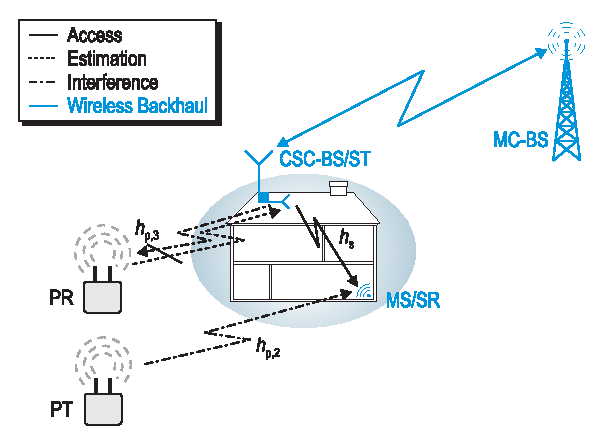
\includegraphics[width = \figscalet]{figures/CR_Scenario_Underlay}
%\vspace{-6mm}
\caption{A cognitive small cell scenario demonstrating: (i) the underlay paradigm, (ii) the associated network elements, which constitute Cognitive Small Cell-Base Station/Secondary Transmitter (CSC-BS/ST), Mobile Station/Secondary Receiver (MS/SR), Macro Cell-Base Station (MC-BS) and Primary Transmitter (PT), (iii) the interacting channels: primary interference channel, secondary interference channel and access channel.}
\label{fig_US:scenario}
%\vspace{-4mm}
\end{figure}
%\subsubsection{Medium access}

\subsection{Underlay Scenario and Medium Access}

%The Cognitive Small Cell (CSC), a CR application, characterizes a small cell deployment that fulfills the spectral requirements of the Mobile Stations (MSs) operating indoor, refer to \figurename~\ref{fig_US:scenario}.
%For the disposition of the CSC in the network, the following key elements are essential: a CSC-Base Station (CSC-BS), a Macro Cell-Base Station (MC-BS) and an MS. 
Considering the fact that the power control is employed at the CSC-BS, the CSC-BS and the MS represent the ST and the SR, respectively. In order to acquire channel knowledge concerning the primary interference channel, the ST listens to the transmissions from the PR, refer to \figurename~\ref{fig_US:scenario}. In this chapter, those primary systems where the PR\footnote{Clearly, it is ambiguous to consider transmissions from a PR, different terms such as primary radio or simply primary user can be used instead. Since the main focus is to characterize the interference at the PR, it is sensible to use the nomenclature PR.} performs transmissions interchangeably over time (time division duplexing TDD and half-duplex frequency division duplexing FDD) or frequency (full-duplex FDD) with the PT are considered. These transmissions can occur over the same band (TDD) or over separate bands (half-duplex and full-duplex FDD). 
%The ST follows these duplexing modes to transmit signals with controlled power over the access channel. 
In cellular networks, these duplexing modes are effectively deployed in the Long Term Evolution (LTE) standard \cite{LTE09}. The ST follows these duplexing modes to exploit channel reciprocity principle and determine the interference (power) received at the PR, thus, controls its power for transmitting signals over the access channel such that it satisfies the interference constraint by operating at the IT. Particularly for half-duplex and full duplex FDD, it is assumed that the coherence bandwidth is large as compared to frequency separation between the estimation channel and the band of interest. 
%In addition, considering the deployment scenario, due to the outside walls, the SR encounters a loss of $\SI{20}{dB}$ in the received power, 
%Cognitive Relay (CR) \cite{Kaushik14} characterizes a small cell deployment that fulfills the spectral requirements for Indoor Devices (IDs). \figurename~\ref{fig_US:scenario} illustrates a snapshot of a CR scenario to depict the interaction between the CR with PR and ID, where CR and ID represents the ST and SR respectively. In \cite{Kaushik14}, the challenges involved while deploying the CR as US were presented. However for simplification, a constant transmit power was considered at the CR. Now, we extend the analysis to employ power control at the ST. 
%\begin{figure}[!ht]
%\centering
%\includegraphics[width = \figscalet]{figures/Frame_Structure_ink}
%\vspace{-6mm}
%\caption{The proposed frame structure of underlay system channel estimation for the interference channel.}
%\label{fig_US:fs}
%\vspace{-11mm}
%\end{figure}
\begin{figure}[!ht]
\centering
\includegraphics[width = \columnwidth]{figures/Frame_Structure}
\caption{Frame structure of the USs illustrating the time allocation for channel estimation and data transmission from the perspective of a ST and a SR. Corresponding to the uplink and the downlink, the primary interference channel and secondary interference channel estimation occur at the ST and the SR, respectively. PR (Tx)/PR (Rx) presents the transmission/reception of the primary signal from the PR/PT to the PT/PR.} 
\label{fig_US:fs}
%\vspace{-7mm}
\end{figure}



A slotted medium access for the US is considered, where the time axis is segmented into frames. As depicted in \figurename~\ref{fig_US:fs}, the frame duration $T$ is chosen in such a way that the frames are aligned to the PUs' transmissions. In order to incorporate channel estimation, a periodic channel estimation\footnote{This frame structure is similar to the periodic sensing followed by the interweave systems \cite{Liang08}.} is proposed, according to which, the US uses a time interval $\test (< T)$ to perform channel estimation followed by data transmission $T- \test$, see \figurename~\ref{fig_US:fs}. Besides, to consider variations due to channel fading, it is assumed that the interacting channels remain constant at least over two frame durations ($2T$). Based on this assumption, every alternating transmission frame observes a different received power, consider \figurename~\ref{fig_US:fs}. Since the channel knowledge is essential to employ power control such that the PRs are sufficiently protected from the uncertain interference induced due to imperfect channel knowledge, it is reasonable to carry out estimation for $\test$ time interval followed by data transmission with power control in the remaining time $T - \test$ for each frame. %At the end, the remaining time $T - \test$ is utilized for data transmission with controlled power. 

In accordance with the half duplexing modes, the ST and the SR perform received power-based estimation to acquire the knowledge of the primary and the secondary interference channel over consecutive frames, as illustrated in \figurename~\ref{fig_US:fs}. For primary systems and secondary systems that implement full-duplex FDD, the proposed frame structure can be adapted such that the estimation of the primary and the secondary interference channels occurs in a single frame. Besides this, the access channel estimation is performed by listening to the pilot symbols from the SR depicted as a pilot-based estimation. 
%Considering the fact that the number of pilot symbols is relatively small in comparison to the samples used for performing received power-based channel estimation, the time allocation of the pilot symbols does not affect the overall performance of the USs. Hence, no time resources are allocated for access channel estimation in the frame structure.
At first, the proposed frame structure in context to the deterministic behavior of the interacting channels (deterministic channel) is considered, i.e., the performance is analyzed for a certain channel gain (path-loss channel), without taking into account the effect of channel fading. Next, the performance analysis of the proposed framework is carried out by taking channel fading into account (random channel). %In accordance with the nature of regulatory policies, the aforementioned analyses can be considered for deploying the underlay CR systems. 



%To simplify the analysis, we assume that during data transmission at the ST, the interference at the SR, from the PT, to be below the noise level. However, by replacing the noise power with interference plus noise power in the throughput expressions, derived later in Section \ref{sec_US:et_ana}, the performance of the US under the interference limited regime can be depicted. %In this view, the interaction with the PT is excluded in the considered scenario, cf. \figurename~\ref{fig_US:scenario}. 

\subsection{Signal Model}
In the uplink, during the estimation phase, the discrete and complex signal received from the PR at the ST is given by
\begin{equation}
\yrcvd[n] = \hpth \cdot \xtran[n] + \wsr[n],
\label{eq_US:sys_mod_st}
\end{equation}
where $\xtran[n]$ corresponds to a discrete and complex sample transmitted by the PR with transmit power $\ptran$ known at the ST, $\phpth$ represents the power gain for the interference channel and $\wsr[n]$ is circularly symmetric AWGN at the ST with %The transmitted power at PR is $\ptran$, considering that $\test \fsam$ $(= N)$ is the number of samples used for estimation. 
$\mathcal{CN}(0, \nps)$. %The power received at the ST is given as 
%\begin{align}
%\prcvd = \s{\test \fsam}{ |\sqrt{\gp \ap} \xtran[n] + \nas[n]|^2}.
%\label{eq_US:prcvd} 
%\end{align}

In the downlink, during data transmission phase, the signal received at the PR is given by
\begin{equation}
\yp[n] = \hpth  \cdot \xreg[n] + \wpr[n],
\label{eq_US:sys_mod_pr}
\end{equation}
and on the other side, the received signal at the SR follows 
\begin{equation}
\ys[n] = \gs \cdot \xreg[n] + \gpt \cdot \xp[n] + \wsr[n],
\label{eq_US:sys_mod_sr}
\end{equation}
where $\xreg[n]$ corresponds to a discrete and complex sample transmitted by the ST with controlled power $\preg$, and $\xp[n]$ is the transmit signal from the PT with transmit power $\ptranpt$. In reference to the proposed framework, the knowledge of the transmit power at the PT is not necessary at the secondary system. Hence, its ignorance at the SR doesn't affect the analysis concerning the secondary interference. Further, $\pgs$ and $\pgpt$ represent the power gain for the access channel and the secondary interference channel, respectively. $\wpr[n]$ and $\wsr[n]$ are AWGN at the PR and at the SR, respectively, with $\mathcal{CN}(0, \nps)$.%\footnote{In practice, the noise power at the ST, the SR and the PR have different values. The fact is, only the signal to noise ratio received at the ST, and SR and the PR, respectively, are affected due to these noise powers. Since these signal to noise ratios are already included in the performance analysis, the assignment of different notations to these noise powers are excluded in the expressions.} 
%Considering (\ref{eq_US:sys_mod_pr}), the powers received at the PR and SR are evaluated as $\pp = \s{(T - \test) \fsam}{|\yp[n]^2|}$ and $\ps = \s{(T - \test) \fsam}{|\yp[n]^2|}$. Likewise (\ref{eq_US:sys_mod_st}), $\nap[n]$ and $\nas[n]$ represents circularly symmetric AWGN at PR and ST with zero mean and variance $\e{}{|\nap[n]|^2} = \npp$ and $\e{}{|\nas[n]|^2} = \nps$ correspondingly. Consider that $\ptran$, $\preg$ and $\pp$ correspond to power for a given frame. 
%\subsubsection{Channel}

%We consider that all transmitted signals are subjected to distance dependent path loss. The small scale fading gains $\gp, \gs$ are modelled as frequency-flat fading. Hence, the $\gp, \gs$ follow an exponential distribution \cite{Tse05} where $\e{}{\gp}$ and $\e{}{\gs}$ represent their path loss.

\subsection{Problem Description} \label{ssec_US:pd}
According to the existing investigations (also referred as ideal model), an ST of an US is required to control its transmit power in such a way that the interference received $\prcvdpr$ at the PR is below IT ($\ite$) \cite{Xing07}
\begin{equation}
\prcvdpr = \phpth \preg \le \ite.
\label{eq_US:IT_id}
\end{equation}
%where $\alpha$ denotes the distance dependent path loss. $g\sub{p}$ represents the small-scale channel fading. 

After determining the controlled power at the ST using (\ref{eq_US:IT_id}), the data rate at the SR is defined as
\begin{equation}
\ca = \log_2 \left(1 + \frac{\pgs \preg}{ \pgpt \ptranpt + \nps} \right). 
\label{eq_US:Thr_id}
\end{equation}
where $\ca$ represents the data rate over the access channel. %\footnote{From a communication theoretic point of view.}.
%where $\e{\gs, \gp}{\cdot}$ represents the expectation over $\gs, \gp$.
From the deployment perspective, the ideal model depicted in (\ref{eq_US:IT_id}) and (\ref{eq_US:Thr_id}) has following issues:
\begin{itemize}
\item Without the knowledge of the primary interference channel $\hpth$, it is impossible to employ the power control based on (\ref{eq_US:IT_id}). 
\item Furthermore, along with $\preg$, the knowledge of the access channel $\gs$ and the secondary interference channel $\gpt$ is required to determine $\ca$ according to (\ref{eq_US:Thr_id}).
\end{itemize}
The ideal model considers the perfect knowledge of the aforementioned channels at the ST, which is not available in practice. In this regard, it is necessary to incorporate channel estimation in the system model. The imperfect channel knowledge, however, translates to the variations in the performance parameters, $\prcvdpr$ and $\ca$. Particularly, the variations in $\prcvdpr$ that exceed $\ite$ cause uncertain interference at the PR, thereby violating the interference constraint illustrated in (\ref{eq_US:IT_id}). Unless captured, this uncertain interference may seriously degrade the performance of the US. In addition, since the ideal model assumes the perfect knowledge of the involved channels, it fails to depict the degradation in the performance due to the time resources allocated for the channel estimation. %In this view, we characterize the variations in $\pp$ and $\trs$ by characterizing the distribution functions of the estimated channels.

\subsection{Proposed Approach} 
In order to facilitate channel estimation for the USs, it is essential to take the aforementioned issues into account. To accomplish this, the following strategy is proposed in this chapter.
\begin{itemize}
\item At first, the estimation of involved channels is considered. In this regard, a received power-based estimation for the interference channels and a pilot-based estimation for the access channel is employed. 
\item To capture the effect of the imperfect channel knowledge, the variations in the estimated parameters (namely, received power for the interference channels and power gain for the access channels) are characterized in terms of their cumulative distribution functions.
\item Further, the aforementioned variations are translated to the performance parameters, such as the interference at the PR and the secondary throughput in terms of their cumulative distribution functions. More specifically, using the characterization of the uncertain interference, a novel power control mechanism based on an outage control is proposed that regulates the uncertain interference at the PR.  
\item Finally, using the derived expressions, a relationship between the estimation time and the expected secondary throughput for the USs is analyzed. The proposed framework (also referred as estimation model) is further extended to analyze the impact of channel fading on the performance of the system. 
\end{itemize}
Since the channel estimation in the context of CR systems involves two different (primary and secondary) systems, suitable channel estimation techniques should be selected such that the following requirements: (i) low complexity and (ii) versatility towards unknown PU signals, essential from the deployment perspective, are respected. Similar problem for the interweave CR systems has been deeply investigated in Chapter \ref{chap:IS}, where it proposes to employ a received power-based estimation for the channels between the primary and the secondary users and a pilot-based estimation for the access channel. In contrast to this, in this chapter, the received power-based and the pilot-based estimation techniques are applied in the underlay CR systems. It is also worth stating that, since the signal model in Chapter \ref{chap:IS} (OFDM transmission) differs from the one (constant power transmission) studied in this chapter, new mathematical expressions for the performance parameters are derived. 
In the following paragraphs, the estimation of the power gains of the primary interference channel $\ephpth$, the access channel $\epgs$ and the secondary interference channel $\epgpt$ is considered. 
\subsubsection{Estimation of primary interference channel}
Considering
\begin{equation}
\prcvdstpr = \pgpth \ptran + \nps \label{eq_US:prcvd}, 
\end{equation}
and the knowledge of PR's transmit power $\ptran$, the ST employs received power-based estimation to obtain the knowledge of $\pgpth$. To accomplish this, in reference to (\ref{eq_US:sys_mod_st}), the ST listens to the transmissions from the PR and acquires the knowledge of $\epgpth$ indirectly by estimating the power received in the uplink as $\eprcvdstpr = \s{\test \fsam}{|\yrcvd[n]|^2}$, where $\fsam$ being the sampling frequency and $\test$ represents the estimation time interval. 
%$\fsam$ and $\test$ are such that the number of samples $\test \fsam$ is an integer. 
The estimated received power $\eprcvdstpr$ is utilized to determine the control power $\preg$ at which the data transmission over the downlink is carried out, \figurename~\ref{fig_US:fs}. In accordance to the received power-based estimation for the channel $\pgpth$, it is noticed that the knowledge of $\ptran$ at the ST is essential for the characterization of the controlled power (considered later in Lemma \ref{lm_US:lm4}). However, this knowledge can be retrieved by considering the specifications of different wireless standards such GSM, EDGE and LTE, etc. \cite{Sharma14}. It is well-known that certain standards (considered as primary systems) follow adaptive modulation and coding, which can consequently change $\ptran$. Under this situation, the ST can employ more complex techniques such as pilot assisted techniques in order to determine $\ptran$ for the given frame.

For a certain value of $\pgpth$, the received power at the ST estimated using $\test \fsam$ samples, refer to (\ref{eq_US:prcvd}), follows a non-central chi-squared distribution $\fprcvdstpr \sim \ncchi2(\lpth, \test \fsam)$ with non-centrality parameter $\lpth = \test \fsam \phpth \times$ $\ptran /\nps = \test \fsam \snrrcvdu$ \cite{Kay}, where $\snrrcvdu$ is defined as the ratio of the received power (from the PR) to noise at the ST and $\test \fsam$ corresponds to the degrees of freedom. In order to sustain analytical tractability in the analysis, the Approximation \ref{ap:ap1} presented in Chapter \ref{chap:IS} is considered. 
%\begin{approxi} \label{ap:ap1}
%\normalfont
%For all degrees of freedom, the $\ncchi2$ distribution can be approximated by a Gamma distribution \cite{abramo}. The parameters of the Gamma distribution are obtained by matching the first two central moments to those of $\ncchi2$.
%\end{approxi}
\begin{lemma} \label{lm_US:lm1}
\normalfont
The cumulative distribution function of $\eprcvdstpr$ is characterized as 
\begin{align}
\fprcvdstpr(x) \approx 1 - \Gamma&\left(\apo, \frac{x}{\bpo}\right) \label{eq_US:fprcvd}, \\ 
\text{where  } \apo = \frac{\test \fsam (1 + \snrrcvdu)^2}{2 + 4 \snrrcvdu} &\text{ and } \bpo = \frac{\nps (2 + 4 \snrrcvdu)}{\test \fsam (1 + \snrrcvdu)},  \label{eq_US:para_po} 
\end{align} 
and $\Gamma(\cdot, \cdot)$ represents the regularized upper-incomplete Gamma function \cite{abramo}. 
\end{lemma}
\begin{IEEEproof}
Applying Approximation \ref{ap:ap1} from Chapter \ref{chap:IS} to $\ncchi2(\lpth, \test \fsam)$ yields (\ref{eq_US:fprcvd}). 
\end{IEEEproof}

\subsubsection{Estimation of access channel}
Analog to Chapter \ref{chap:US} In the uplink, the pilot signal transmitted by the SR undergoes matched filtering and demodulation at the ST, hence, a pilot-based estimation is employed at the ST to acquire the knowledge of the access channel. %According to \cite{Gifford08}, the maximum-likelihood estimate with $\Ks$ pilot symbols is given by 
%\begin{align}
%\gs = \egs + \frac{\sum^{\Ks}_{n} p[n]}{2 \Ks},
%\label{eq_US:pilot_MLE}
%\end{align}
%where $p[n]$ denotes the discrete pilot symbol and $\frac{\sum^{\Ks}_{n} p[n]}{2 \Ks}$ represents the estimation error. With no loss of generality, the pilot symbols are considered to be $+1$.
%(\ref{eq_US:pilot_MLE}) illustrates a correlation between the $\hs$ and $\ehs$. 
%As a result, the estimate $\egs$ is unbiased, efficient, i.e., achieves the Cram\'er-Rao bound with equality, with asymptotic variance $\e{}{|\gs -\egs|^2} = \frac{\nps}{2 \Ks}$ \cite{Gifford08}. 
Hence, $\egs$ conditioned on $\gs$ follows a Gaussian distribution
\begin{align}
\egs|\gs \sim \mathcal{N}\left( \gs,\frac{\nps}{2 \Ks} \right).
\label{eq_US:ehs} 
\end{align}
Consequently, for a certain value $\phs$ the estimated power gain $|\egs|^2$ follows a non-central chi-squared $\ncchi2(\ls, 1)$ distribution with 1 degree of freedom and non-centrality parameter $\ls = \frac{2 \Ks |\gs|^2}{\nps}$. 
\begin{lemma} \label{lm_US:lm2}
\normalfont
The cumulative distribution function of $\epgs$ is characterized as 
\begin{align}
\fgs(x) \approx 1 - \Gamma&\left(\as, \frac{x}{\bs}\right) \label{eq_US:fehs},\\ 
\text{where  } \as = \frac{(1 + \ls)^2}{2 + 4 \ls} &\text{ and } \bs = \frac{\nps (2 + 4 \ls)}{(1 + \ls)}. \label{eq_US:para_s} 
\end{align} 
\end{lemma}
\begin{IEEEproof}
Applying Approximation \ref{ap:ap1} from Chapter \ref{chap:IS} to $\ncchi2(\ls,1 )$ yields (\ref{eq_US:fehs}). 
\end{IEEEproof}

\subsubsection{Estimation of secondary interference channel}
%In the downlink, the SR cancels the ST the data signal over the access channel in order to estimate the secondary interference (power) received from the PT, refer to (\ref{eq_US:sys_mod_sr}). In order to establish a preliminary analysis, it is assumed that signal to noise ratio for the access link is suitable enough to allow perfect cancellation of the data signal. For extreme situations, a probabilistic approach can be applied to deal with the imperfect signal cancellation for the proposed channel estimation. However, under such situations, it is possible that due to bad quality of the access channel, the ST may not consider such a channel for data transmission. 
The power estimated over the signal $\hpth \xp[n] + \wsr[n]$ corresponds to the interference plus noise power ($\prcvdsr = \pgpt \ptranpt + \nps$, where $\prcvdsr$ represents the true value, consider (\ref{eq_US:Thr_id})). The estimated received power at the SR is determined as $\eprcvdsr = \s{\test \fsam}{|\gpth \cdot \xtranpr[n] + \wsr[n]|^2}$. To characterize the secondary throughput, $\eprcvdsr$ is made available to the ST over a low rate feedback channel. Similar to $\eprcvdstpr$, for a certain value of $\phpt$, $\eprcvdsr$ follows a non-central chi-squared distribution $\ncchi2(\lpt, \test \fsam)$, with non-centrality parameter $\lpt = \test \fsam \pgpt \ptranpt / \nps$.
\begin{lemma} \label{lm_US:lm3}
\normalfont
The cumulative distribution function of $\eprcvdstpr$ is characterized as 
\begin{align}
\fprcvdsr(x) \approx 1 - \Gamma&\left(\apt, \frac{x}{\bpt}\right) \label{eq_US:fprcvdsr}, \\ 
\text{where  } \apt = \frac{(\test \fsam + \lpt)^2}{2 \test \fsam + 4 \lpt} &\text{ and } \bpt = \frac{\nps (2 \test \fsam + 4 \lpt)}{(\test \fsam + \lpt)}.  \label{eq_US:para_pt} 
\end{align} 
\end{lemma}
\begin{IEEEproof}
Applying Approximation \ref{ap:ap1} from Chapter \ref{chap:IS} to $\ncchi2(\lpt, \test \fsam)$ yields (\ref{eq_US:fprcvdsr}). 
\end{IEEEproof}
\begin{remark}
\normalfont
It is important to note that, the scenario described in this chapter considers a single PT and a single PR. However, in practice, it is possible that the ST and the SR accumulate significant interference (defined as aggregate interference) from other PRs and PTs (co-channel interference due to frequency reuse) in the network\cite{Elsawy13_cmag,Kaushik14_P} over the primary interference channel and the secondary interference channel, respectively. For the secondary interference channel, the only difference is that the SR now estimates the aggregate interference. Due to this, the expression of $\eprcvdsr$ in the throughput remains unchanged. On the other side, by estimating the aggregate interference on the primary interference channel, the ST overestimates $\eprcvdstpr$ and exercises a greater power control. Even for such a case, the outage constraint on the primary interference channel to the desired PR is satisfied, which consequently reduces the secondary throughput.  
\end{remark}
%%%%%%%%%%%%%%%%%%%%%%%%%%%%%%%%%%%%%%%%%%%%%%%%%%%%%%%%%%%%%%%%%%%%%%%%%%%%%%%%%%%%%%%%%
\section{Theoretical Analysis} \label{sec_US:th_ana}
%%%%%%%%%%%%%%%%%%%%%%%%%%%%%%%%%%%%%%%%%%%%%%%%%%%%%%%%%%%%%%%%%%%%%%%%%%%%%%%%%%%%%%%%%

%%%%%%%%%%%%%%%%%%%%%%%%%%%%%%%%%%%%%%%%%%%%%%%%%%%%%%%%%%%%%%%%%%%%%%%%%%%%%%%%%%%%%%%%%
\subsection{Deterministic Channel} \label{ssec_US:stpa}
%%%%%%%%%%%%%%%%%%%%%%%%%%%%%%%%%%%%%%%%%%%%%%%%%%%%%%%%%%%%%%%%%%%%%%%%%%%%%%%%%%%%%%%%%

%\subsection{Short-term Analysis}
%We first investigate the short-term analysis, whereby the channel is $\gp, \gs$ to a and unknown.
%  desired by the regulatory bodies, we capture this variation by means of an outage probability constraint $\p(\pp \ge \ite) \le \opc$.  %, it is impthrtant for the system to restrain $\op$ above a certain desired level $\opc$. %As a result, the outage probability constraint is defined as
%\begin{align}
%\p(\pp = \gp \preg \ge \ite) \le \opd. 
%\label{eq_US:opc} 
%\end{align} 
%\begin{lemma}
%The controlled power that satisfies 
%\end{lemma}
%\subsubsection{Power control}
%Given $\test$ is utilized for $\prcvd$ estimation, the throughput at the SR is given by  
%\begin{equation}
%\rs(\test) = \frac{T - \test}{T} \log_2 \left(1 + \frac{\gs \preg(\test) }{\nps} \right). 
%\label{eq_US:Thr_pm}
%\end{equation}
%It will be clear later in this section that small $\test$ results in large variations for the $\prcvd$ and vice versa. According to (\ref{eq_US:preg}), this induces variations in $\preg$. These variations causes $\pp$ to deviate from $\ite$. If not considered in the model, these variations may affect the performance of the system. 
%Based on (\ref{eq_US:opc}), the controlled power at the PR is determined as 
%\begin{align}
%\preg(\test) = \ite \cdot F_{\frac{1}{\gp}}^{-1}(\opd, \test), 
%\label{eq_US:preg}
%\end{align}
%where $\mathcal{F}_{\frac{1}{\gp}}^{-1}$ represents the inverse-distribution function of $1/{\gp}$.
%Clearly, there exits a tradeoff that involves maximizing the expected throughput at the SR subject to a outage probability constraint is given by 
Here, the performance of the USs is investigated on a single-frame basis. In this sense, the involved channels $\hpth$, $\gpt$ and $\gs$ are considered to be deterministic.   
At first, an outage probability constraint
%\footnote{The outage constraint is commonly used parameter for designing communication system that ensures the outage occurs no more than a certain percentage of time.} 
$\opc$ on the uncertain interference is employed to capture the variations in the $\prcvdpr$ incurred due to channel estimation, defined as 
\begin{align}
\p\left( \prcvdpr = \ephpth \preg \ge \ite \right) \le \opc. 
\intertext{Substituting $\ephpth$ from (\ref{eq_US:prcvd}) yields}
\p\left( \left( \frac{\eprcvdstpr - \nps}{\ptran}\right) \preg \ge \ite \right) \le \opc. \label{eq_US:opc} \\[-1em] \nonumber 
\end{align}
Besides the outage constraint, $\preg$ is limited by a predefined transmit power $\pc$. To capture this aspect, the transmit power constraint at the ST is defined as
\begin{align}
\preg \le \pc. \label{eq_US:pc} 
\end{align} 
It is considered that the same power is allocated to all the symbols transmitted within a frame by the ST. In this regard, the transmit power constraint on symbol basis and frame basis is equivalent. As a consequence, the constraint depicted in (\ref{eq_US:pc}) is applicable to both the scenarios. Based on the constraints in (\ref{eq_US:opc}) and (\ref{eq_US:pc}), an expression of the controlled power for the proposed framework is determined.
\begin{lemma} \label{lm_US:lm4}
\normalfont 
Subject to the outage constraint on the uncertain interference and the transmit power constraint at the ST, the controlled power at the ST is given by
\begin{align}
\preg &= 
\begin{cases} 
\frac{\ite \ptran}{ \left(\bpo \Gamma^{-1}(\opc, \apo) - \nps  \right)} & \mbox{if } \preg < \pc \\
\pc & \mbox{if } \preg \ge \pc
\end{cases},
\label{eq_US:preg} 
\end{align}
where $\apo$ and $\bpo$ are defined in (\ref{eq_US:para_po}).
\end{lemma} 
\begin{IEEEproof}
Substituting the cdf for $\eprcvdstpr$, defined in (\ref{eq_US:fprcvd}), in (\ref{eq_US:opc}) and combining with (\ref{eq_US:pc}) yields (\ref{eq_US:preg}).
\end{IEEEproof}
Clearly, the performance of the US improves over the access channel (in terms of the secondary throughput) with $\preg$, but $\preg$ increases for the values of $\phpth$, which correspond to the lower values of $\snrrcvdu$.
The real world wireless systems are limited by the transmit power $\pc$, which bounds the performance of the USs. In order to understand the effect of the power limitation on the USs, a performance bound is characterized in terms of the estimation time and the signal to noise ratio received (from the PR) at the ST\footnote{\tc{Signal to noise ratio is mostly used as a design parameter for characterizing the performance of a wireless system.}}.  
 
\begin{coro} \label{cor_US:cor1}
\normalfont
Subject to the outage constraint on the uncertain interference and the transmit power constraint at the ST, the performance bound ($\snrrcvdu^*$) of the USs is defined as %\footnote{Please note that $\test \fsam$ and $\snrrcvd$ are included in the parameters $\apo$ and $\bpo$, refer to (\ref{eq_US:para_po}).} 
\begin{align}
\Gamma\left(\frac{\test \fsam (1 + \snrrcvdu^*)^2}{2 + 4 \snrrcvdu^*}, \frac{\test \fsam (1  + \snrrcvdu^*)}{\nps (2 + 4 \snrrcvdu^*)} \left( \frac{\ite \ptran}{\pc} + \nps  \right)  \right) = \opc. \label{eq_US:opreg}  
\end{align}
\end{coro}
\begin{IEEEproof}
Substituting $\preg$ with $\pc$ in (\ref{eq_US:opc}) and reformulating gives 
\begin{align}
%\p\left( \left( \frac{\eprcvd - \nps}{\ptran}\right) \pc \ge \ite \right) \le \opc 
\p\left( \eprcvdstpr \ge \frac{\ite \ptran}{\pc} + \nps \right) &\le \opc. \label{eq_US:opreg_a} 
\end{align}
Using (\ref{eq_US:fprcvd}) in Lemma \ref{lm_US:lm1} gives
\begin{align}
\Gamma\left(\frac{\test \fsam (1 + \snrrcvdu)^2}{2 + 4 \snrrcvdu}, \frac{\test \fsam (1  + \snrrcvdu)}{\nps (2 + 4 \snrrcvdu)} \left( \frac{\ite \ptran}{\pc} + \nps  \right)  \right) &\le \opc. \label{eq_US:opreg_b} 
\end{align}
Substituting $\snrrcvdu$ with $\snrrcvdu^*$ and replacing the expression in (\ref{eq_US:opreg_b}) with equality yields (\ref{eq_US:opreg}). 
\end{IEEEproof}
\begin{figure}[!ht]
%\vspace{-5mm}
%% Add psfrag entries
% This file is generated by the MATLAB m-file laprint.m. It can be included
% into LaTeX documents using the packages graphicx, color and psfrag.
% It is accompanied by a postscript file. A sample LaTeX file is:
%    \documentclass{article}\usepackage{graphicx,color,psfrag}
%    \begin{document}% This file is generated by the MATLAB m-file laprint.m. It can be included
% into LaTeX documents using the packages graphicx, color and psfrag.
% It is accompanied by a postscript file. A sample LaTeX file is:
%    \documentclass{article}\usepackage{graphicx,color,psfrag}
%    \begin{document}% This file is generated by the MATLAB m-file laprint.m. It can be included
% into LaTeX documents using the packages graphicx, color and psfrag.
% It is accompanied by a postscript file. A sample LaTeX file is:
%    \documentclass{article}\usepackage{graphicx,color,psfrag}
%    \begin{document}\input{fig_N_vs_SNR_diff_pout_diff_maxContPow_th}\end{document}
% See http://www.mathworks.de/matlabcentral/fileexchange/loadFile.do?objectId=4638
% for recent versions of laprint.m.
%
% created by:           LaPrint version 3.16 (13.9.2004)
% created on:           06-Jan-2016 16:54:20
% eps bounding box:     16 cm x 12 cm
% comment:              
%
%\begin{psfrags}%
%\psfragscanon%
%
% text strings:
\psfrag{s03}[b][b]{\fontsize{8.5}{12.75}\fontseries{m}\mathversion{normal}\fontshape{n}\selectfont \color[rgb]{0,0,0}\setlength{\tabcolsep}{0pt}\begin{tabular}{c}$\tau$ [ms]\end{tabular}}%
\psfrag{s04}[t][t]{\fontsize{8.5}{12.75}\fontseries{m}\mathversion{normal}\fontshape{n}\selectfont \color[rgb]{0,0,0}\setlength{\tabcolsep}{0pt}\begin{tabular}{c}$\snrrcvd$ [dB]\end{tabular}}%
%
% axes font properties:
\fontsize{8.5}{12.75}\fontseries{m}\mathversion{normal}%
\fontshape{n}\selectfont%
%
% xticklabels:
\psfrag{x01}[t][t]{-20}%
\psfrag{x02}[t][t]{-15}%
\psfrag{x03}[t][t]{-10}%
\psfrag{x04}[t][t]{-5}%
%
% yticklabels:
\psfrag{v01}[r][r]{0}%
\psfrag{v02}[r][r]{2}%
\psfrag{v03}[r][r]{4}%
\psfrag{v04}[r][r]{6}%
\psfrag{v05}[r][r]{8}%
\psfrag{v06}[r][r]{10}%
\psfrag{v07}[r][r]{12}%
\psfrag{v08}[r][r]{14}%
\psfrag{v09}[r][r]{16}%
\psfrag{v10}[r][r]{18}%
\psfrag{v11}[r][r]{20}%
%
% Figure:
%\resizebox{8cm}{!}{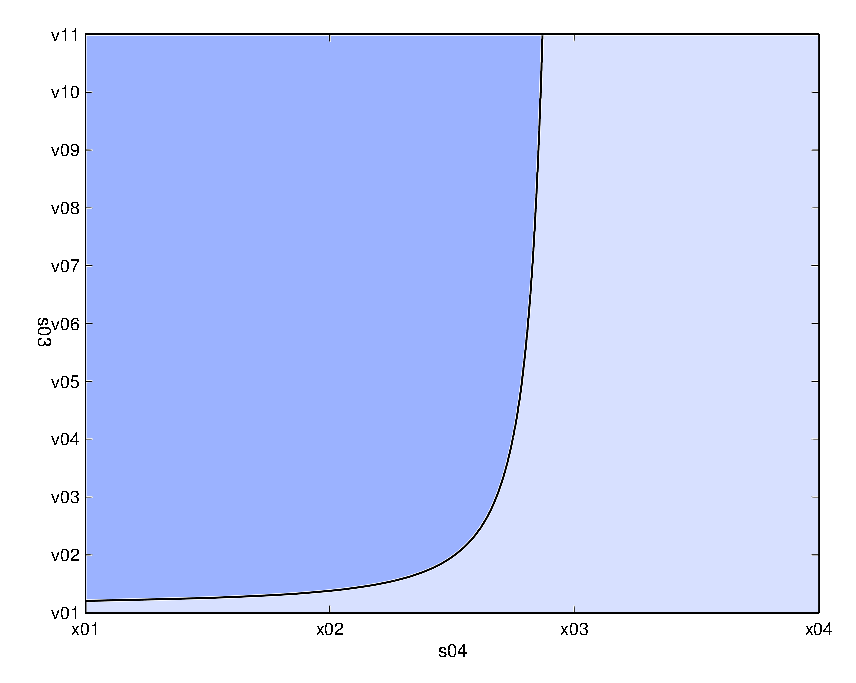
\includegraphics{fig_N_vs_SNR_diff_pout_diff_maxContPow_th.eps}}%
%\end{psfrags}%
%
% End fig_N_vs_SNR_diff_pout_diff_maxContPow_th.tex
\end{document}
% See http://www.mathworks.de/matlabcentral/fileexchange/loadFile.do?objectId=4638
% for recent versions of laprint.m.
%
% created by:           LaPrint version 3.16 (13.9.2004)
% created on:           06-Jan-2016 16:54:20
% eps bounding box:     16 cm x 12 cm
% comment:              
%
%\begin{psfrags}%
%\psfragscanon%
%
% text strings:
\psfrag{s03}[b][b]{\fontsize{8.5}{12.75}\fontseries{m}\mathversion{normal}\fontshape{n}\selectfont \color[rgb]{0,0,0}\setlength{\tabcolsep}{0pt}\begin{tabular}{c}$\tau$ [ms]\end{tabular}}%
\psfrag{s04}[t][t]{\fontsize{8.5}{12.75}\fontseries{m}\mathversion{normal}\fontshape{n}\selectfont \color[rgb]{0,0,0}\setlength{\tabcolsep}{0pt}\begin{tabular}{c}$\snrrcvd$ [dB]\end{tabular}}%
%
% axes font properties:
\fontsize{8.5}{12.75}\fontseries{m}\mathversion{normal}%
\fontshape{n}\selectfont%
%
% xticklabels:
\psfrag{x01}[t][t]{-20}%
\psfrag{x02}[t][t]{-15}%
\psfrag{x03}[t][t]{-10}%
\psfrag{x04}[t][t]{-5}%
%
% yticklabels:
\psfrag{v01}[r][r]{0}%
\psfrag{v02}[r][r]{2}%
\psfrag{v03}[r][r]{4}%
\psfrag{v04}[r][r]{6}%
\psfrag{v05}[r][r]{8}%
\psfrag{v06}[r][r]{10}%
\psfrag{v07}[r][r]{12}%
\psfrag{v08}[r][r]{14}%
\psfrag{v09}[r][r]{16}%
\psfrag{v10}[r][r]{18}%
\psfrag{v11}[r][r]{20}%
%
% Figure:
%\resizebox{8cm}{!}{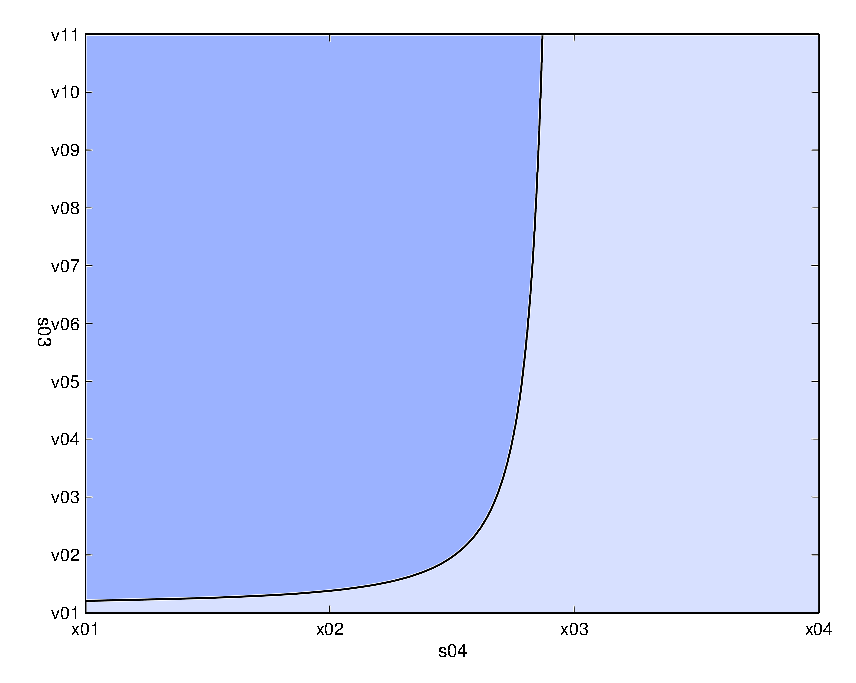
\includegraphics{fig_N_vs_SNR_diff_pout_diff_maxContPow_th.eps}}%
%\end{psfrags}%
%
% End fig_N_vs_SNR_diff_pout_diff_maxContPow_th.tex
\end{document}
% See http://www.mathworks.de/matlabcentral/fileexchange/loadFile.do?objectId=4638
% for recent versions of laprint.m.
%
% created by:           LaPrint version 3.16 (13.9.2004)
% created on:           06-Jan-2016 16:54:20
% eps bounding box:     16 cm x 12 cm
% comment:              
%
%\begin{psfrags}%
%\psfragscanon%
%
% text strings:
\psfrag{s03}[b][b]{\fontsize{8.5}{12.75}\fontseries{m}\mathversion{normal}\fontshape{n}\selectfont \color[rgb]{0,0,0}\setlength{\tabcolsep}{0pt}\begin{tabular}{c}$\tau$ [ms]\end{tabular}}%
\psfrag{s04}[t][t]{\fontsize{8.5}{12.75}\fontseries{m}\mathversion{normal}\fontshape{n}\selectfont \color[rgb]{0,0,0}\setlength{\tabcolsep}{0pt}\begin{tabular}{c}$\snrrcvd$ [dB]\end{tabular}}%
%
% axes font properties:
\fontsize{8.5}{12.75}\fontseries{m}\mathversion{normal}%
\fontshape{n}\selectfont%
%
% xticklabels:
\psfrag{x01}[t][t]{-20}%
\psfrag{x02}[t][t]{-15}%
\psfrag{x03}[t][t]{-10}%
\psfrag{x04}[t][t]{-5}%
%
% yticklabels:
\psfrag{v01}[r][r]{0}%
\psfrag{v02}[r][r]{2}%
\psfrag{v03}[r][r]{4}%
\psfrag{v04}[r][r]{6}%
\psfrag{v05}[r][r]{8}%
\psfrag{v06}[r][r]{10}%
\psfrag{v07}[r][r]{12}%
\psfrag{v08}[r][r]{14}%
\psfrag{v09}[r][r]{16}%
\psfrag{v10}[r][r]{18}%
\psfrag{v11}[r][r]{20}%
%
% Figure:
%\resizebox{8cm}{!}{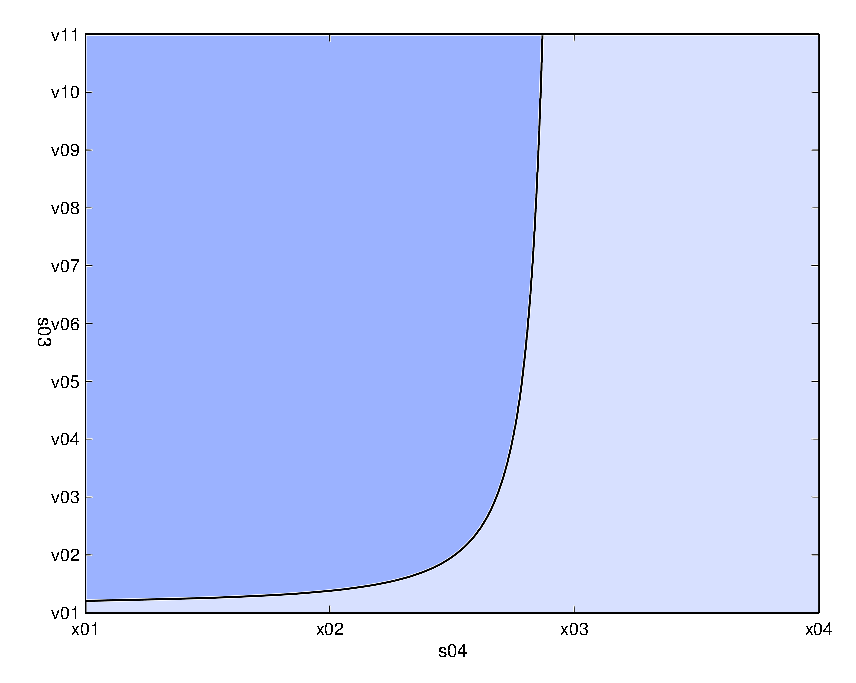
\includegraphics{fig_N_vs_SNR_diff_pout_diff_maxContPow_th.eps}}%
%\end{psfrags}%
%
% End fig_N_vs_SNR_diff_pout_diff_maxContPow_th.tex

\centering
\begin{tikzpicture}[scale=1]
\node[anchor=south west,inner sep=0] (image) at (0,0)
{
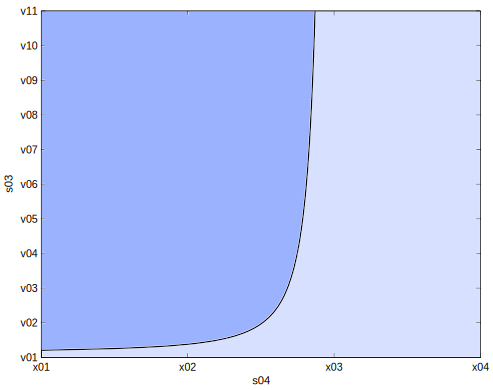
\includegraphics[width= \figscale]{figures/fig_N_vs_SNR_diff_pout_diff_maxContPow_th}
};
\begin{scope}[x={(image.south east)},y={(image.north west)}]

%\draw (0.86,0.42) arc(-250:70:0.04 and 0.02);
%\node[draw,fill=gray!10,font=\scriptsize] (text1) at (0.65,0.4) {$\pc = \SI{-10}{dBm}$};
%\draw[black, <-] (text1.east) -- (0.835,0.4);
%\draw (0.42,0.7) arc(-250:70:0.04 and 0.02);
%\node[draw,fill=gray!10,font=\scriptsize] (text2) at (0.65,0.68) {$\pc = \SI{0}{dBm}$};
%\draw[black, <-] (text2.west) -- (0.475,0.68);

\draw (0.62,0.75) arc(-250:70:0.03 and 0.015);
\node[draw,fill=gray!0,font=\scriptsize] (text1) at (0.56,0.735) {$\snrrcvdu^*$}; 
%\draw[black, <-] (text1.east) -- (0.46,0.7);
\node[draw,fill=gray!0,font=\scriptsize] at (0.8,0.53) {Interference-limited};
\node[draw,fill=gray!0,font=\scriptsize] at (0.35,0.53) {Power-limited};

%\draw[help lines,xstep=.1,ystep=.1] (0,0) grid (1,1);
%\foreach \x in {0,1,...,9} { \node [anchor=north] at (\x/10,0) {0.\x}; }
%\foreach \y in {0,1,...,9} { \node [anchor=east] at (0,\y/10) {0.\y}; }
\end{scope}
\end{tikzpicture}

%\vspace{-4mm}
\caption{
An illustration of the performance bound ($\snrrcvdu^*$) for the US depicted in terms of estimation time ($\tau$) and the ratio of the received power (from the PR) to noise ($\snrrcvdu$) at the ST. It further classifies the operation of the USs as the interference-limited and the power-limited regimes.}
\label{fig_US:or}
%\vspace{-10mm}
\end{figure}
\begin{remark} \label{rm_US:rm1}
\normalfont
\figurename~\ref{fig_US:or} analyzes the variations of $\snrrcvdu^*$ with $\test$. Using the expression $\snrrcvdu^*$ obtained in Corollary \ref{cor_US:cor1}, the operation of the USs into the following regimes is classified: (i) interference-limited regime and (ii) power-limited regime. \tc{Inside the interference-limited regime $\snrrcvdu > \snrrcvdu^*$, due to good quality of the channel ST-PR (unfavorable to the USs), the system is limited due to the exceeding level of the uncertain interference, which can be regulated effectively by employing power control at the US to satisfy the given outage constraint. At $\snrrcvdu = \snrrcvdu^*$, the ST operates at the maximum allowable power $\preg = \pc$ while respecting the tolerance limits defined for the uncertain interference. From a different perspective, the situation $\snrrcvdu = \snrrcvdu^*$ also represents those USs that are unable to carry out power control. With regard to the outage constraint and the lack of the power control, for a given choice of $\snrrcvdu^*$, such systems can operate only at a specific value of $\test$.
%At $\snrrcvdu = \snrrcvdu^*$, the system operates at the maximum transmit power $\pc$, i.e., without power control. It is worth noticing that the situation $\snrrcvdu = \snrrcvdu^*$ is a representative of those underlay systems that are unable to carry out power control. With regard to desired outage constraint on the uncertain interference, such systems can operate for a given choice of $\snrrcvdu^*$ only at a certain value of $\test$. From a different perspective, at $\snrrcvdu = \snrrcvdu^*$, the USs are allowed to operate with maximum transmit power $\pc$ without exceeding the tolerance limits defined for the interference. 
}

\tc{
On the other side, the region $\snrrcvdu \le \snrrcvdu^*$, which depicts a weak link quality between the ST and the PR, hence, is beneficial to the secondary user. However, due to the transmit power constraint, the USs are confined to operate at $\pc$. As a result, these favorable conditions do not translate to any performance gain.} Therefore, this regime is characterized as a power-limited regime. \tc{Besides, it is interesting to observe that for low values of the estimation time, $\snrrcvdu^* \rightarrow -\infty$, which signifies that low $\test$ increases the uncertainty in the interference. In order to regulate the level of this uncertainty, US has to be proactive in terms of power control mechanism to be able to satisfy the interference constraint. It is also observed that as $\test \rightarrow \infty$, $\snrrcvdu^*$ converges asymptotically to a certain value. This signifies the fact that additional time resources allocated for the channel estimation, after a certain value, does not account to any significant improvement in the terms of the uncertain interference, or indirectly power control. As a result, the performance of the US in the form of power control gets saturated.}  %As a result, by replacing $\snrrcvdu^*$ in the following expression of secondary throughput, we determine the performance limits of operation for the US. 
\end{remark}
%Based on the operation regime, we determine best performance, in terms of the lowest operational SNR, achieved by the US. 
Next, the variations in the secondary throughput are captured in terms of its expected value. To accomplish this, the cdf of the data rate%\footnote{\tc{Please note, the following terms the data rate $\ca$ and the throughput $\rs$ have been introduced to make a clear distinction between the instantaneous data rate and its average value over the frame duration.}}
\begin{align}
\eca  = \log_2 \left(1 + \frac{\epgs \preg}{\eprcvdsr} \right) \label{eq_US:eca}
\end{align}
is evaluated over the access channel at the ST. It is worth noticing the fact that unlike $\ca$ defined in (\ref{eq_US:Thr_id}), $\eca$ entails the random behavior due to the estimation of $\epgs$ and $\eprcvdsr$.
\begin{lemma} \label{lm_US:lm5}
\normalfont 
The cdf of data rate $\eca$ is given by
\begin{align}
\fc(x) &= \int\limits_{0}^{x} \dc(t) dt, \label{eq_US:dis_C} 
\end{align}
where the $\dc(x)$ probability density function (pdf) is given by 
\begin{align}
\dc(x) &= 2^x \ln 2 \frac{(2^x - 1)^{\as - 1} \Gamma(\as + \apt)}{\Gamma(\as) \Gamma(\apt) (\bs \ptran) ^{\as} \bpt^{\apt}} \left(\frac{1}{\bpt} + \frac{2^x - 1}{\bs \ptran}\right). \label{eq_US:den_C}
\end{align}
\end{lemma}
\begin{IEEEproof}
See Appendix \ref{ap:one}.
\end{IEEEproof}

\captionsetup[subfigure]{position=top}
\begin{figure}[!ht]
\centering
\subfloat[]{
% This file is generated by the MATLAB m-file laprint.m. It can be included
% into LaTeX documents using the packages graphicx, color and psfrag.
% It is accompanied by a postscript file. A sample LaTeX file is:
%    \documentclass{article}\usepackage{graphicx,color,psfrag}
%    \begin{document}\input{fig_CDF_Cs_diff_SNR_p2}\end{document}
% See http://www.mathworks.de/matlabcentral/fileexchange/loadFile.do?objectId=4638
% for recent versions of laprint.m.
%
% created by:           LaPrint version 3.16 (13.9.2004)
% created on:           13-Jan-2016 19:02:56
% eps bounding box:     16 cm x 12 cm
% comment:              
%
%\begin{psfrags}%
%\psfragscanon%
%
% text strings:
\psfrag{s05}[t][t]{\fontsize{8}{12}\fontseries{m}\mathversion{normal}\fontshape{n}\selectfont \color[rgb]{0,0,0}\setlength{\tabcolsep}{0pt}\begin{tabular}{c}$\eca$ [bits/sec/Hz]\end{tabular}}%
\psfrag{s06}[b][b]{\fontsize{8}{12}\fontseries{m}\mathversion{normal}\fontshape{n}\selectfont \color[rgb]{0,0,0}\setlength{\tabcolsep}{0pt}\begin{tabular}{c}CDF\end{tabular}}%
\psfrag{s10}[][]{\fontsize{10}{15}\fontseries{m}\mathversion{normal}\fontshape{n}\selectfont \color[rgb]{0,0,0}\setlength{\tabcolsep}{0pt}\begin{tabular}{c} \end{tabular}}%
\psfrag{s11}[][]{\fontsize{10}{15}\fontseries{m}\mathversion{normal}\fontshape{n}\selectfont \color[rgb]{0,0,0}\setlength{\tabcolsep}{0pt}\begin{tabular}{c} \end{tabular}}%
\psfrag{s12}[l][l]{\fontsize{8}{12}\fontseries{m}\mathversion{normal}\fontshape{n}\selectfont \color[rgb]{0,0,0}Simulated}%
\psfrag{s13}[l][l]{\fontsize{8}{12}\fontseries{m}\mathversion{normal}\fontshape{n}\selectfont \color[rgb]{0,0,0}(\ref{eq_US:dis_C})}%
\psfrag{s14}[l][l]{\fontsize{8}{12}\fontseries{m}\mathversion{normal}\fontshape{n}\selectfont \color[rgb]{0,0,0}Simulated}%
%
% axes font properties:
\fontsize{8}{12}\fontseries{m}\mathversion{normal}%
\fontshape{n}\selectfont%
%
% xticklabels:
\psfrag{x01}[t][t]{3}%
\psfrag{x02}[t][t]{3.5}%
\psfrag{x03}[t][t]{4}%
\psfrag{x04}[t][t]{4.5}%
\psfrag{x05}[t][t]{5}%
\psfrag{x06}[t][t]{5.5}%
\psfrag{x07}[t][t]{6}%
\psfrag{x08}[t][t]{6.5}%
%
% yticklabels:
\psfrag{v01}[r][r]{0}%
\psfrag{v02}[r][r]{0.1}%
\psfrag{v03}[r][r]{0.2}%
\psfrag{v04}[r][r]{0.3}%
\psfrag{v05}[r][r]{0.4}%
\psfrag{v06}[r][r]{0.5}%
\psfrag{v07}[r][r]{0.6}%
\psfrag{v08}[r][r]{0.7}%
\psfrag{v09}[r][r]{0.8}%
\psfrag{v10}[r][r]{0.9}%
%
% Figure:
%\resizebox{8cm}{!}{\includegraphics{fig_CDF_Cs_diff_SNR_p2.eps}}%
%\end{psfrags}%
%
% End fig_CDF_Cs_diff_SNR_p2.tex


\begin{tikzpicture}[scale=1]
\node[anchor=south west,inner sep=0] (image) at (0,0)
{
        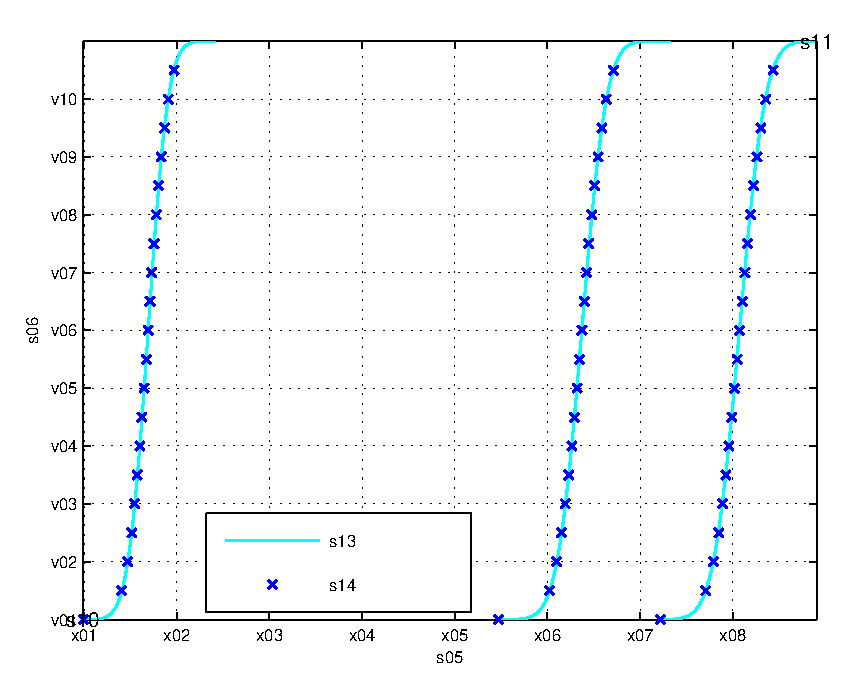
\includegraphics[width = \figscale]{figures/fig_CDF_Cs_diff_SNR_p2_AWGN} 
};
\begin{scope}[x={(image.south east)},y={(image.north west)}]

\draw (0.848,0.4) arc(-250:70:0.04 and 0.02);
\node[draw,fill=gray!10,font=\scriptsize] (text1) at (0.43,0.38) {$\frac{\pgpt \ptranpt}{\nps} = \SI{-10}{dB}$};
\draw[black, <-] (text1.east) -- (0.822,0.38);
\draw (0.672,0.6) arc(-250:70:0.04 and 0.02);
\node[draw,fill=gray!10,font=\scriptsize] (text2) at (0.43,0.58) {$\frac{\pgpt \ptranpt}{\nps} = \SI{0}{dB}$};
\draw[black, <-] (text2.east) -- (0.646,0.58);
\draw (0.162,0.8) arc(-250:70:0.04 and 0.02);
\node[draw,fill=gray!10,font=\scriptsize] (text3) at (0.43,0.78) {$\frac{\pgpt \ptranpt}{\nps} = \SI{10}{dB}$};
\draw[black, <-] (text3.west) -- (0.216,0.78);


%\draw[help lines,xstep=.1,ystep=.1] (0,0) grid (1,1);
%\foreach \x in {0,1,...,9} { \node [anchor=north] at (\x/10,0) {0.\x}; }
%\foreach \y in {0,1,...,9} { \node [anchor=east] at (0,\y/10) {0.\y}; }
\end{scope}
\end{tikzpicture}

\label{fig_US:CDF_C1_s}}
\hfil
\subfloat[]{
% This file is generated by the MATLAB m-file laprint.m. It can be included
% into LaTeX documents using the packages graphicx, color and psfrag.
% It is accompanied by a postscript file. A sample LaTeX file is:
%    \documentclass{article}\usepackage{graphicx,color,psfrag}
%    \begin{document}\input{fig_CDF_Cs_diff_Np2}\end{document}
% See http://www.mathworks.de/matlabcentral/fileexchange/loadFile.do?objectId=4638
% for recent versions of laprint.m.
%
% created by:           LaPrint version 3.16 (13.9.2004)
% created on:           13-Jan-2016 19:01:11
% eps bounding box:     16 cm x 12 cm
% comment:              
%
%\begin{psfrags}%
%\psfragscanon%
%
% text strings:
\psfrag{s05}[t][t]{\fontsize{8}{12}\fontseries{m}\mathversion{normal}\fontshape{n}\selectfont \color[rgb]{0,0,0}\setlength{\tabcolsep}{0pt}\begin{tabular}{c}$\eca$ [bits/sec/Hz]\end{tabular}}%
\psfrag{s06}[b][b]{\fontsize{8}{12}\fontseries{m}\mathversion{normal}\fontshape{n}\selectfont \color[rgb]{0,0,0}\setlength{\tabcolsep}{0pt}\begin{tabular}{c}CDF\end{tabular}}%
\psfrag{s10}[][]{\fontsize{10}{15}\fontseries{m}\mathversion{normal}\fontshape{n}\selectfont \color[rgb]{0,0,0}\setlength{\tabcolsep}{0pt}\begin{tabular}{c} \end{tabular}}%
\psfrag{s11}[][]{\fontsize{10}{15}\fontseries{m}\mathversion{normal}\fontshape{n}\selectfont \color[rgb]{0,0,0}\setlength{\tabcolsep}{0pt}\begin{tabular}{c} \end{tabular}}%
\psfrag{s12}[l][l]{\fontsize{8}{12}\fontseries{m}\mathversion{normal}\fontshape{n}\selectfont \color[rgb]{0,0,0}Simulated}%
\psfrag{s13}[l][l]{\fontsize{8}{12}\fontseries{m}\mathversion{normal}\fontshape{n}\selectfont \color[rgb]{0,0,0}Theoretical}%
\psfrag{s14}[l][l]{\fontsize{8}{12}\fontseries{m}\mathversion{normal}\fontshape{n}\selectfont \color[rgb]{0,0,0}Simulated}%
%
% axes font properties:
\fontsize{8}{12}\fontseries{m}\mathversion{normal}%
\fontshape{n}\selectfont%
%
% xticklabels:
\psfrag{x01}[t][t]{6}%
\psfrag{x02}[t][t]{6.2}%
\psfrag{x03}[t][t]{6.4}%
\psfrag{x04}[t][t]{6.6}%
\psfrag{x05}[t][t]{6.8}%
\psfrag{x06}[t][t]{7}%
\psfrag{x07}[t][t]{7.2}%
\psfrag{x08}[t][t]{7.4}%
%
% yticklabels:
\psfrag{v01}[r][r]{0}%
\psfrag{v02}[r][r]{0.1}%
\psfrag{v03}[r][r]{0.2}%
\psfrag{v04}[r][r]{0.3}%
\psfrag{v05}[r][r]{0.4}%
\psfrag{v06}[r][r]{0.5}%
\psfrag{v07}[r][r]{0.6}%
\psfrag{v08}[r][r]{0.7}%
\psfrag{v09}[r][r]{0.8}%
\psfrag{v10}[r][r]{0.9}%
%
% Figure:
%\resizebox{8cm}{!}{\includegraphics{fig_CDF_Cs_diff_Np2.eps}}%
%\end{psfrags}%
%
% End fig_CDF_Cs_diff_Np2.tex
 
\begin{tikzpicture}[scale=1]
\node[anchor=south west,inner sep=0] (image) at (0,0)
{
        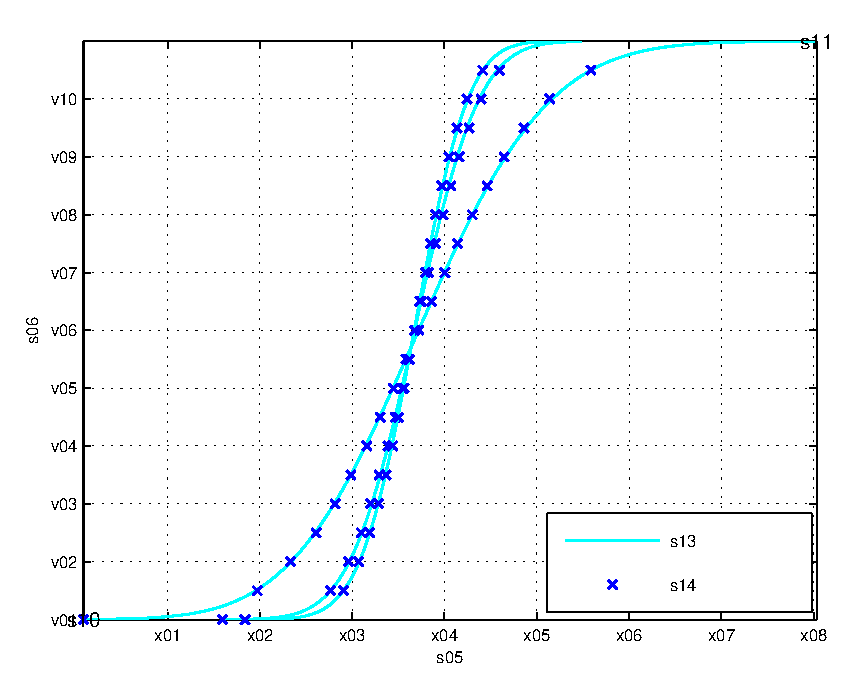
\includegraphics[width = \figscale]{figures/fig_CDF_Cs_diff_Np2_AWGN} 
};
\begin{scope}[x={(image.south east)},y={(image.north west)}]

\draw[black,->] (0.28,0.25) -- (0.48,0.15);
\node[draw=none, font=\scriptsize] at (0.25,0.3) {$\test \in \{0.1,1,10\} \SI{}{ms}$};

%\draw[help lines,xstep=.1,ystep=.1] (0,0) grid (1,1);
%\foreach \x in {0,1,...,9} { \node [anchor=north] at (\x/10,0) {0.\x}; }
%\foreach \y in {0,1,...,9} { \node [anchor=east] at (0,\y/10) {0.\y}; }
\end{scope}
\end{tikzpicture}
\label{fig_US:CDF_C1_p2}}
\vspace{0.3cm}
\caption{CDF of $\eca$ for different $\pgpt \ptranpt/\nps$ and $\test$. (a) $\pgpt \ptranpt/\nps \in \{-10, 0, 10\} \SI{}{dB}$ and $\test = \SI{1}{ms}$, (b) $\test \in \{0.1, 1, 10\} \SI{}{ms}$ and $\pgpt \ptranpt/\nps = \SI{0}{dB}$.}%, for the following values of system parameters, $\snrrcvdu = \SI{10}{dB}$, $\preg = \SI{0}{dBm}$.}
\label{fig_US:CDF_eca}
\vspace{-0.5cm}
\end{figure}
In consideration to the Approximation \ref{ap:ap1}, which is applied to obtain the cdfs' of $\eprcvdstpr$, $\epgs$ and $\eprcvdsr$ in Lemma \ref{lm_US:lm5}, the theoretical expression of the cdf depicted in (\ref{eq_US:dis_C}) is validated by means of simulations in \figurename~\ref{fig_US:CDF_eca} with different choices of system parameters, which include signal to noise ratio over the primary interference channel at the ST $\snrrcvdu = \SI{10}{dB}$, controlled power $\preg = \SI{0}{dBm}$, interference to noise ratio at the SR over the secondary interference channel $\frac{\pgpt \ptranpt}{\nps} \in \{-10, 0, 10\} \SI{}{dB}$ and estimation time $\test \in \{0.1, 1, 10\} \SI{}{ms}$.

Besides the outage constraint on the uncertain interference, the expected secondary throughput over the access channel at the SR is defined as
\begin{align}
\rs(\test) %&= \e{\epgs, \eprcvdsr} {\frac{T - \test}{T} \log_2 \left(1 + \frac{\epgs \preg }{\eprcvdsr} \right)}, \label{eq_US:rs}
          &= \frac{T - \test}{T} \e{\eca} {\eca}, \label{eq_US:rs}
\end{align} 
where $\e{\eca}{\cdot}$ corresponds to an expectation over $\eca$, whose pdf is characterized in Lemma \ref{lm_US:lm5}. 

\begin{remark} \label{rm_US:rm3}
\normalfont
\tc{At this point, it is well-known that the performance degradation due to channel estimation in the form of the secondary throughput is inherent to the USs. Specifically, the time allocation and the uncertain interference are responsible of this degradation. The power control, determined in Lemma \ref{lm_US:lm4}, represented as a function of estimation time is able to regulate the uncertain interference. As discussed previously in Remark \ref{rm_US:rm1}, the low estimation time enables a severe control in power, thereby reducing the secondary throughput. On the other hand, the time resources allocated for the channel estimation also decrease the throughput. This phenomenon can be captured by observing the variation of the secondary throughput along the estimation time such that the constraints depicted in (\ref{eq_US:opc}) and (\ref{eq_US:pc}) are fulfilled. Below, Problem \ref{th_US:th1} captures this relationship between the estimation time and the secondary throughput defined as estimation-throughput tradeoff. More importantly, this tradeoff is utilized to determine a suitable estimation time at which maximum throughput at the SR is achieved.}
\end{remark}
\begin{theorem} \label{th_US:th1}
\normalfont
The expected achievable secondary throughput subject to the outage constraint on the uncertain interference and the transmit power constraint at the ST is defined as
\begin{align}
\trs(\ttest)  = \maxi_{\test}  & \text{      } {\rs(\test)}, 
 \label{eq_US:sys} \\
\text{s.t.} & \text{ } (\ref{eq_US:opc}), \text{  } (\ref{eq_US:pc}), \nonumber 
%\text{s.t.} & \text{ } \p\left( \left( \frac{\eprcvd - \nps}{\ptran} \right) \preg \ge \ite \right) \le \opc, \nonumber \\ 
%\text{s.t.} & \text{ }  \preg \le \pc, \nonumber   
 \end{align}
where $\trs(\ttest)$ corresponds to optimum throughput at $\ttest$.  
\end{theorem}
\begin{IEEEproof}
The constrained optimization problem is solved by substituting $\preg$ from Lemma \ref{lm_US:lm3}, determined by applying the outage and the transmit power constraints defined in (\ref{eq_US:opc}) and (\ref{eq_US:pc}), in (\ref{eq_US:rs}). 
The pdf of $\eca$, determined in (\ref{eq_US:den_C}), is used to evaluate the expectation on the secondary throughput. Following this, an expression of the expected secondary throughput as a function of $\test$\footnote{Please note that the model parameters $\apt$ and $\bpt$, defined in (\ref{eq_US:para_pt}), used for characterizing pdf of $\eca$ in (\ref{eq_US:den_C}) are functions of $\test$.} is determined as
\begin{equation}
\rs(\test) = \frac{T - \test}{T} \int\limits_{0}^{\infty} x \dc(x) dx. \label{eq_US:intrs}
\end{equation}
Solving numerically the expression in (\ref{eq_US:intrs}) yields $\ttest$ and $\trs(\ttest)$. 
\end{IEEEproof}
\begin{coro} \label{cor_US:cor2}
\normalfont
Problem \ref{th_US:th1} considers the optimization of the expected secondary throughput for the proposed framework that employ power control and considers the effect of the imperfect channel knowledge. \tc{In accordance to Corollary \ref{cor_US:cor1}, these USs correspond to the ones that operate in the interference-limited regime $\snrrcvdu^* \ge \snrrcvdu $.} Besides, it is interesting to compare its performance with those USs that employ channel estimation and satisfy the outage constraint on the uncertain interference, however, employ no power control, i.e., operate at $\pc$. \tc{With regard to Corollary \ref{cor_US:cor1}, these systems correspond to the ones operating on the curve $\snrrcvdu^*  = \snrrcvdu$. For the latter approach, the secondary throughput is obtained by substituting $\preg$ with $\pc$ in (\ref{eq_US:rs}), where $\test$ in (\ref{eq_US:rs}) is determined using Corollary \ref{cor_US:cor1}. Such a comparison allows us to quantify the performance gain procured by the USs through the employment of power control.}
\end{coro}

%Problem \ref{th_US:th1} depicts an optimum estimation time $\ttest$ that achieves an optimum secondary throughput $\trs(\ttest)$.
%The throughput depicted from (\ref{eq_US:Thr_id}) for the ideal model overestimates the throughput of the US. %This overestimation in the throughput is evaluated as $\beta$ that depicts the difference between the $\ers$ obtained from the models. 
%It is evident that for analyzing the tradeoff depicted in (\ref{eq_US:sys}), first it is impthrtant to characterize the $\preg$ and density function $\drs$. 

%\subsection{Short term analysis}
%To simplify the analysis, we consider a case where the transmitted signals are subject to path loss only, that is, the small scale channel gains correspond to $\gs = \gp = 1$. In this way, we first consider the variations in $\pp$ due to the presence of noise in the system. 

%\subsubsection{Characterization of performance parameters}
%Considering (\ref{eq_US:prcvd}), $\prcvd$ follows a non-central chi-squared distributed $\mathcal{X'}^2(N \snrrcvdu, N)$, where $\snrrcvd = \ptran/\nps$ denotes the received SNR \cite{Urkowitz}. 
%According to (\ref{eq_US:preg}), $\preg$ for the short term case is given by 



%%%%%%%%%%%%%%%%%%%%%%%%%%%%%%%%%%%%%%%%%%%%%%%%%%%%%%%%%%%%%%%%%%%%%%%%%%%%%%%%%%%%%%%%%
\subsection{Random Channel}\label{ssec_US:ltpa}
%%%%%%%%%%%%%%%%%%%%%%%%%%%%%%%%%%%%%%%%%%%%%%%%%%%%%%%%%%%%%%%%%%%%%%%%%%%%%%%%%%%%%%%%%
Here, the objective is to investigate the performance of the proposed approach, where the interacting channels encounter quasi-static block fading. Following the frame structure in \figurename~\ref{fig_US:fs}, the alternating transmissions observe a different channel. In this regard, the channel gains $\hpth$, $\gpt$ and $\gs$ are characterized according to Nakagami-$m$ fading model. Analog to the previous chapter, the power gains $\phpth$, $\pgpt$ and $\pgs$ follow a Gamma distribution \cite{Goldsmith05}, whose corresponding cumulative distribution functions are defined as  
\begin{align}
\fpgpth(x) = 1 - \Gamma\left(\mpth, \frac{\mpth x}{\bpgpth}\right), \label{eq_US:dis_pgpth}\\
\fpgpt(x) = 1 - \Gamma\left(\mpt, \frac{\mpt x}{\bpgpt}\right), \label{eq_US:dis_pgpt}\\  
\fpgs(x) = 1 - \Gamma\left(\ms , \frac{\ms x}{\bpgs}\right), \label{eq_US:dis_pgs}
\end{align}
where $\mpth$, $\mpt$ and $\ms$ represent the $m$ parameter, whereas $\bpgpth$, $\bpgpt$ and $\bpgs$ are the expected values for channels $\pgpth$, $\pgpt$ and $\pgs$, respectively. %$\Gamma(\cdot, \cdot)$ is a regularized upper-incomplete Gamma function \cite{abramo}.
The performance analysis subject to channel fading has been considered by Ghasemi \textit{et al.} \cite{Ghasemi06, Ghasemi07}. However, the authors in \cite{Ghasemi06, Ghasemi07} evaluated average data rate under an average interference constraint. The influence of the channel fading (however, without channel estimation) has been quantified in terms of the outage constraint on the uncertain interference\footnote{The uncertainty is interference power received at the PR is due to channel fading.}, is given by %. In order to make a fair comparison (benchmark) of our proposed approach, the ideal model the existing investigations in context to channel fading are quantified based on an outage constraint on the primary interference, given by
\begin{align}
	\max_{\preg} & \e{\pgpt, \pgs }{ \frac{\pgs \preg}{\pgpt \ptranpt + \nps}} \label{eq_US:sys_id_fad}, \\
	\text{s.t.} & \text{ } \p(\prcvdpr= \phpth \preg \ge \ite) \le \opc, \label{eq_US:opc_id_fad} 
\end{align}
where $\e{\pgpt, \pgs} {\cdot}$ corresponds to expectation with respect to $\pgpt$, $\pgs$.
Despite the knowledge of the fading model, similar to the ideal model depicted for the deterministic channel (refer to Section \ref{ssec_US:pd}), the characterization in (\ref{eq_US:sys_id_fad}) and (\ref{eq_US:opc_id_fad}) assumes the perfect knowledge of the different realizations of the power gains $(\phpth, \pgpt, \pgs)$ of the corresponding channels. In view of this, subsequently, the proposed framework is further extended to investigate the effect of the random channel (channel fading) on the performance of the USs that incorporates estimation of the involved channels.

Firstly, the expression of the outage constraint on the uncertain interference is determined as 
\begin{align}
\smash[b]{\overbrace{\e{\phpth}{\smash[b]{\underbrace{\p\left( \left( \frac{\eprcvdstpr- \nps}{\ptran}\right) \preg \ge \ite \right)}_{\text{Channel Estimation}}}}}^{\text{Channel Fading}}} \le \opc, \label{eq_US:opc_fad} \\[0.5em] \nonumber 
\end{align}
where $\eprcvdstpr$ depends on the underlying value of $\phpth$. In contrast to the constraint in (\ref{eq_US:opc_id_fad}) defined for the models considering perfect channel knowledge, (\ref{eq_US:opc_fad}) captures the variations due to the channel estimation $(\p(\cdot)$ determined in terms of $\eprcvdstpr$) and the channel fading ($\e{\phpth}{\cdot}$). Based on (\ref{eq_US:opc_fad}) and transmit power constraint defined in (\ref{eq_US:pc}), it is essential to derive the expression of the controlled power $(\preg)$ for the case with random channel.

\begin{lemma} \label{lm_US:lm6}
\normalfont
Subject to the outage constraint on the uncertain interference and the transmit power constraint at the ST, the controlled power at the ST under Nakagami-$m$ fading is given by %(see top of next page (\ref{eq_US:preg_fad}))
%\begin{figure*}[!ht]

%\begin{sideways}
%\begin{minipage}{14.85cm}
%\begin{center}
\begin{align}
&\preg = \nonumber \\ 
& \begin{cases} 
\text{Solving for $\preg$, } \\ \int\limits_{0}^{\infty} \Gamma\bigg(\frac{\test \fsam (1 + x \ptran/\nps)^2}{2 + 4 x \ptran/\nps}, \frac{\test \fsam (1 + x \ptran/\nps)}{\nps (2 + 4 x \ptran/\nps)} \\ \bigg(\frac{\ite\ptran}{\preg}  +  \nps \bigg)\bigg) d \fphpth(x) = \opc & \mbox{if } \preg < \pc \\
\pc & \mbox{if } \preg \ge \pc
\end{cases}
\label{eq_US:preg_fad} 
\end{align}
%\end{center}
%\end{minipage}
%\end{sideways}
%\hrulefill
%\end{figure*}
, where %$\apo$ and $\bpo$ are defined in (\ref{eq_US:para_po}) and 
$\fphpth(\cdot)$ is defined in (\ref{eq_US:dis_pgpth}). 
\end{lemma} 
\begin{IEEEproof}
Since it is complicated to obtain a closed form expression of the integral in (\ref{eq_US:preg_fad}), therefore, the controlled power is evaluated numerically.  
\end{IEEEproof}
Similar to deterministic channel (in Corollary \ref{cor_US:cor1}), below, the performance bound $(\snrrcvdu^*)$ in terms of $\snrrcvdu$ and $\test$ for the random channel is determined.
 $\snrrcvdu^*$ is determined by substituting $\preg$ with $\pc$ in the expression (\ref{eq_US:preg_fad}) 
\begin{align}
%\hspace{-4mm}
&\int\limits_{0}^{\infty} \Gamma\left( \frac{\test \fsam (1 + x \ptran/\nps)^2}{2 + 4 x \ptran/\nps}, \frac{\test \fsam (1 + x \ptran/\nps)}{\nps (2 + 4 x \ptran/\nps)}  \left(\frac{\ite\ptran}{\pc} + \nps \right)\right) \nonumber \\ & d \fphpth(x) \le \opc. \label{eq_US:or_fad}
\end{align}
{In order to obtain $\snrrcvdu^*$, the integral on the left side in (\ref{eq_US:or_fad}) is evaluated to obtain function of $\phpth$ and $\test$. Since no closed form expression of this function is obtained, it is represented as}
\begin{align*}
g(\phpth, \test \fsam) \le \opc. \nonumber   
\end{align*}
{Substituting $\phpth = \frac{\snrrcvdu^* \nps}{\ptran}$ and replacing with equality, $\snrrcvdu^*$ for the random channel is determined as} 
\begin{align*}
g\left(\frac{\snrrcvdu^* \nps}{\ptran}, \test \fsam\right) &= \opc. \nonumber  
\end{align*}
\begin{figure}[!ht]

%% Add psfrag entries
% This file is generated by the MATLAB m-file laprint.m. It can be included
% into LaTeX documents using the packages graphicx, color and psfrag.
% It is accompanied by a postscript file. A sample LaTeX file is:
%    \documentclass{article}\usepackage{graphicx,color,psfrag}
%    \begin{document}% This file is generated by the MATLAB m-file laprint.m. It can be included
% into LaTeX documents using the packages graphicx, color and psfrag.
% It is accompanied by a postscript file. A sample LaTeX file is:
%    \documentclass{article}\usepackage{graphicx,color,psfrag}
%    \begin{document}% This file is generated by the MATLAB m-file laprint.m. It can be included
% into LaTeX documents using the packages graphicx, color and psfrag.
% It is accompanied by a postscript file. A sample LaTeX file is:
%    \documentclass{article}\usepackage{graphicx,color,psfrag}
%    \begin{document}\input{fig_N_vs_SNR_diff_pout_diff_maxContPow_fading_th}\end{document}
% See http://www.mathworks.de/matlabcentral/fileexchange/loadFile.do?objectId=4638
% for recent versions of laprint.m.
%
% created by:           LaPrint version 3.16 (13.9.2004)
% created on:           06-Jan-2016 11:22:04
% eps bounding box:     16 cm x 12 cm
% comment:              
%
%\begin{psfrags}%
%\psfragscanon%
%
% text strings:
\psfrag{s03}[b][b]{\fontsize{8}{12}\fontseries{m}\mathversion{normal}\fontshape{n}\selectfont \color[rgb]{0,0,0}\setlength{\tabcolsep}{0pt}\begin{tabular}{c}$\tau$ [ms]\end{tabular}}%
\psfrag{s04}[t][t]{\fontsize{8}{12}\fontseries{m}\mathversion{normal}\fontshape{n}\selectfont \color[rgb]{0,0,0}\setlength{\tabcolsep}{0pt}\begin{tabular}{c}$\gamma$ [dB]\end{tabular}}%
%
% axes font properties:
\fontsize{8}{12}\fontseries{m}\mathversion{normal}%
\fontshape{n}\selectfont%
%
% xticklabels:
\psfrag{x01}[t][t]{-20}%
\psfrag{x02}[t][t]{-19}%
\psfrag{x03}[t][t]{-18}%
\psfrag{x04}[t][t]{-17}%
\psfrag{x05}[t][t]{-16}%
\psfrag{x06}[t][t]{-15}%
\psfrag{x07}[t][t]{-14}%
\psfrag{x08}[t][t]{-13}%
\psfrag{x09}[t][t]{-12}%
\psfrag{x10}[t][t]{-11}%
\psfrag{x11}[t][t]{-10}%
%
% yticklabels:
\psfrag{v01}[r][r]{0}%
\psfrag{v02}[r][r]{2}%
\psfrag{v03}[r][r]{4}%
\psfrag{v04}[r][r]{6}%
\psfrag{v05}[r][r]{8}%
\psfrag{v06}[r][r]{10}%
\psfrag{v07}[r][r]{12}%
\psfrag{v08}[r][r]{14}%
\psfrag{v09}[r][r]{16}%
\psfrag{v10}[r][r]{18}%
\psfrag{v11}[r][r]{20}%
%
% Figure:
%\resizebox{8cm}{!}{\includegraphics{fig_N_vs_SNR_diff_pout_diff_maxContPow_fading_th.eps}}%
%\end{psfrags}%
%
% End fig_N_vs_SNR_diff_pout_diff_maxContPow_fading_th.tex
\end{document}
% See http://www.mathworks.de/matlabcentral/fileexchange/loadFile.do?objectId=4638
% for recent versions of laprint.m.
%
% created by:           LaPrint version 3.16 (13.9.2004)
% created on:           06-Jan-2016 11:22:04
% eps bounding box:     16 cm x 12 cm
% comment:              
%
%\begin{psfrags}%
%\psfragscanon%
%
% text strings:
\psfrag{s03}[b][b]{\fontsize{8}{12}\fontseries{m}\mathversion{normal}\fontshape{n}\selectfont \color[rgb]{0,0,0}\setlength{\tabcolsep}{0pt}\begin{tabular}{c}$\tau$ [ms]\end{tabular}}%
\psfrag{s04}[t][t]{\fontsize{8}{12}\fontseries{m}\mathversion{normal}\fontshape{n}\selectfont \color[rgb]{0,0,0}\setlength{\tabcolsep}{0pt}\begin{tabular}{c}$\gamma$ [dB]\end{tabular}}%
%
% axes font properties:
\fontsize{8}{12}\fontseries{m}\mathversion{normal}%
\fontshape{n}\selectfont%
%
% xticklabels:
\psfrag{x01}[t][t]{-20}%
\psfrag{x02}[t][t]{-19}%
\psfrag{x03}[t][t]{-18}%
\psfrag{x04}[t][t]{-17}%
\psfrag{x05}[t][t]{-16}%
\psfrag{x06}[t][t]{-15}%
\psfrag{x07}[t][t]{-14}%
\psfrag{x08}[t][t]{-13}%
\psfrag{x09}[t][t]{-12}%
\psfrag{x10}[t][t]{-11}%
\psfrag{x11}[t][t]{-10}%
%
% yticklabels:
\psfrag{v01}[r][r]{0}%
\psfrag{v02}[r][r]{2}%
\psfrag{v03}[r][r]{4}%
\psfrag{v04}[r][r]{6}%
\psfrag{v05}[r][r]{8}%
\psfrag{v06}[r][r]{10}%
\psfrag{v07}[r][r]{12}%
\psfrag{v08}[r][r]{14}%
\psfrag{v09}[r][r]{16}%
\psfrag{v10}[r][r]{18}%
\psfrag{v11}[r][r]{20}%
%
% Figure:
%\resizebox{8cm}{!}{\includegraphics{fig_N_vs_SNR_diff_pout_diff_maxContPow_fading_th.eps}}%
%\end{psfrags}%
%
% End fig_N_vs_SNR_diff_pout_diff_maxContPow_fading_th.tex
\end{document}
% See http://www.mathworks.de/matlabcentral/fileexchange/loadFile.do?objectId=4638
% for recent versions of laprint.m.
%
% created by:           LaPrint version 3.16 (13.9.2004)
% created on:           06-Jan-2016 11:22:04
% eps bounding box:     16 cm x 12 cm
% comment:              
%
%\begin{psfrags}%
%\psfragscanon%
%
% text strings:
\psfrag{s03}[b][b]{\fontsize{8}{12}\fontseries{m}\mathversion{normal}\fontshape{n}\selectfont \color[rgb]{0,0,0}\setlength{\tabcolsep}{0pt}\begin{tabular}{c}$\tau$ [ms]\end{tabular}}%
\psfrag{s04}[t][t]{\fontsize{8}{12}\fontseries{m}\mathversion{normal}\fontshape{n}\selectfont \color[rgb]{0,0,0}\setlength{\tabcolsep}{0pt}\begin{tabular}{c}$\gamma$ [dB]\end{tabular}}%
%
% axes font properties:
\fontsize{8}{12}\fontseries{m}\mathversion{normal}%
\fontshape{n}\selectfont%
%
% xticklabels:
\psfrag{x01}[t][t]{-20}%
\psfrag{x02}[t][t]{-19}%
\psfrag{x03}[t][t]{-18}%
\psfrag{x04}[t][t]{-17}%
\psfrag{x05}[t][t]{-16}%
\psfrag{x06}[t][t]{-15}%
\psfrag{x07}[t][t]{-14}%
\psfrag{x08}[t][t]{-13}%
\psfrag{x09}[t][t]{-12}%
\psfrag{x10}[t][t]{-11}%
\psfrag{x11}[t][t]{-10}%
%
% yticklabels:
\psfrag{v01}[r][r]{0}%
\psfrag{v02}[r][r]{2}%
\psfrag{v03}[r][r]{4}%
\psfrag{v04}[r][r]{6}%
\psfrag{v05}[r][r]{8}%
\psfrag{v06}[r][r]{10}%
\psfrag{v07}[r][r]{12}%
\psfrag{v08}[r][r]{14}%
\psfrag{v09}[r][r]{16}%
\psfrag{v10}[r][r]{18}%
\psfrag{v11}[r][r]{20}%
%
% Figure:
%\resizebox{8cm}{!}{\includegraphics{fig_N_vs_SNR_diff_pout_diff_maxContPow_fading_th.eps}}%
%\end{psfrags}%
%
% End fig_N_vs_SNR_diff_pout_diff_maxContPow_fading_th.tex

\centering
\begin{tikzpicture}[scale=1]
\node[anchor=south west,inner sep=0] (image) at (0,0)
{
\includegraphics[width= \figscale]{figures/fig_N_vs_SNR_diff_pout_diff_maxContPow_fading_th}
};
\begin{scope}[x={(image.south east)},y={(image.north west)}]

\draw (0.665,0.82) arc(-250:70:0.2 and 0.05);
\node[draw,fill=gray!10,font=\scriptsize] (text1) at (0.505,0.775) {$\snrrcvdu^*$};
%\draw[black,->] (0.12,0.2) node[below=4.0,right=-5.0, rotate = 75, font=\scriptsize] {$m \in \{0.5, 1,2,5, \infty\}$} -- (0.34,0.14);
\draw[black,->] (0.52,0.31) -- (0.85,0.2);
\node[rotate = 75, font=\scriptsize] at (0.5, 0.38) {$m \in \{0.5, 1,2,5, \infty\}$}; 
%\draw[help lines,xstep=.1,ystep=.1] (0,0) grid (1,1);
%\foreach \x in {0,1,...,9} { \node [anchor=north] at (\x/10,0) {0.\x}; }
%\foreach \y in {0,1,...,9} { \node [anchor=east] at (0,\y/10) {0.\y}; }
\end{scope}
\end{tikzpicture}
\caption{An extension of the interference-limited and the power-limited regimes for the US to the random channels, where the channels are subject to Nakagami-$m$ fading. The performance bound ($\snrrcvdu^*$) is depicted in terms of estimation time ($\test$). The different curves demonstrates the severity $(m \in \{0,5,1,2,5, \infty \})$ in fading observed by the primary interference channel.}
\label{fig_US:or_fad}
%\vspace{-5mm}
\end{figure}
\begin{remark} \label{rm_US:rm2}
\normalfont
\figurename~\ref{fig_US:or_fad} analyzes the variation of $\snrrcvdu^*$ with $\test$ for different $m \in \{0.5, 1, 2, 5, \infty\}$, where $m = \infty$ represents a deterministic channel. It is observed that $\snrrcvdu^*$ attains a lower value as fading becomes more severe, hence enables the USs to operate at low $\snrrcvdu$ by extending the interference-limited regime. Following the analysis from Remark \ref{rm_US:rm1}, this also reflects that the power control becomes more proactive as the severity in fading increases. This signifies that power control meant to regulate the uncertainty interference is mainly dominated by variations due to the channel fading for the severely fading channels, in contrast to variations due to channel estimation. In addition, it is noticed that the path-loss channel is more sensitive to the estimation time as compared to the random channels.  
\end{remark}
After determining the controlled power in Lemma \ref{lm_US:lm6} that regulates the uncertain interference, it is essential to determine the expression of the secondary throughput.
\begin{align}
\rs(\test) &= \e{\eca, \pgpt, \pgs} {\frac{T - \test}{T} \eca }, \label{eq_US:rs_fad} 
\end{align} 
where $\e{\eca, \pgpt, \pgs}{\cdot}$ corresponds to an expectation over $\eca$, $\pgpt$ and $\pgs$, whose cdfs are characterized in Lemma \ref{lm_US:lm5}, (\ref{eq_US:dis_pgpt}) and (\ref{eq_US:dis_pgs}), respectively. It is worth noticing that $\eca$ captures the variations due to channel estimation $\epgs$ and $\eprcvdstpr$, refer to (\ref{eq_US:eca}), however due to channel fading, the underlying values of the channels $\pgpt$ and $\pgs$ are random. In this context, an expectation with respect to $\pgpt$ and $\pgs$ as depicted in (\ref{eq_US:rs_fad}) is performed.
Similar to the deterministic channel, the estimation-throughput tradeoff corresponding to the random behaviour of the channels is characterized. 
\begin{theorem} \label{th_US:th2}
\normalfont
The expected achievable secondary throughput subject to the outage constraint on the uncertain interference and the transmit power constraint at the ST under Nakagami-$m$ fading is defined as
\begin{align}
\trs(\ttest) = \maxi_{\test}  & \text{      } {\rs(\test)}, 
 \label{eq_US:sys_fad} \\
\text{s.t.} & \text{ } (\ref{eq_US:opc_fad}), \text{  } (\ref{eq_US:pc}), \nonumber 
%\text{s.t.} & \text{ } \p\left( \left( \frac{\eprcvd - \nps}{\ptran} \right) \preg \ge \ite \right) \le \opc, \nonumber \\ 
%\text{s.t.} & \text{ }  \preg \le \pc, \nonumber   
 \end{align}
where $\trs(\ttest)$ corresponds to optimum secondary throughput at $\ttest$.  
\end{theorem}

\begin{coro} \label{cor_US:cor3}
\normalfont
Here, the approach depicted Corollary \ref{cor_US:cor2} is extended to compare the performance with those CR systems that employ channel estimation, operate with no power control, satisfy the outage constraint and are subjected to Nakagami-$m$ fading. The expected secondary throughput for this particular approach is obtained by replacing $\preg$ in the expression in (\ref{eq_US:rs_fad}) with $\pc$, where $\test$ is determined using (\ref{eq_US:or_fad}). 

\end{coro}
 
%%%%%%%%%%%%%%%%%%%%%%%%%%%%%%%%%%%%%%%%%%%%%%%%%%%%%%%%%%%%%%%%%%%%%%%%%%%%%%%%%%%%%%%%%
\section{Numerical Analysis} \label{sec_US:num_ana}
%%%%%%%%%%%%%%%%%%%%%%%%%%%%%%%%%%%%%%%%%%%%%%%%%%%%%%%%%%%%%%%%%%%%%%%%%%%%%%%%%%%%%%%%%
In this section, the performance of the US based on the proposed estimation model is evaluated. To accomplish this: (i) simulations are performed to validate the expressions obtained, (ii) the performance loss incurred due to the estimation is analyzed. In addition, the ideal model is considered to benchmark and evaluate the performance loss. % (iii) we establish mathematical justification to the considered approximations.
% Unless stated explicitly, the following choice of the parameters is considered for the analysis, cf. Table \ref{tb_US:tb2}.
Unless stated explicitly, the parameters given in Table \ref{tb_US:tb2} are considered for the analysis.%, $\fsam = \SI{1}{MHz}$, $\gp = \SI{-100}{dB}$, $\gs = \SI{-80}{dB}$, $\ite = \SI{-110}{dBm}$, $T = \SI{100}{ms}$, $\opc \in \{0.01, 0.10\}$, $\pc \in \{-10, 0\} \SI{}{dBm}$, $\nps = \SI{-100}{dBm}$, $\snrrcvdu = \SI{0}{dB}$, $\ptran = \SI{0}{dBm}$, $\Ks = 10$.


%\subsection{Short-term analysis}

\begin{table}
%%\vspace{-0.4cm}
\renewcommand{\arraystretch}{1.4}
\caption{Parameters for Numerical Analysis}
%\vspace{-0.6cm}
\label{tb_US:tb2}
\centering
%\scriptsize{
\begin{tabular}{c||c}
\hline
\bfseries Parameter & \bfseries Value \\
\hline\hline
$\fsam$  & $\SI{1}{MHz}$ \\ 
$\phpth$ (or $\bphpth$) & $\SI{-100}{dB}$ \\ 
$\pgpt$ (or $\bpgpt$) & $\SI{-100}{dB}$ \\ 
$\pgs$ (or $\bpgs$) & $\SI{-80}{dB}$ \\ 
$\ite$ & $\SI{-110}{dBm}$ \\ 
$T$ & $\SI{100}{ms}$ \\ 
$\opc$ & 0.10 \\ 
$\pc$ & 0 \SI{}{dBm} \\ 
$\nps$ & $\SI{-100}{dBm}$ \\ 
$\snrrcvdu$ & $\SI{0}{dB}$ \\ 
$\ptran$ & $\SI{0}{dBm}$ \\ 
$\ptranpt$ & $\SI{0}{dBm}$ \\ 
$\Ks$ & 10 \\ 
$m$ & \{1,5\} \\ \hline
\end{tabular}%}
\end{table}

%%%%%%%%%%%%%%%%%%%%%%%%%%%%%%%%%%%%%%%%%%%%%%%%%%%%%%%%%%%%%%%%%%%%%%%%%%%%%%%%%%%%%%%%%
\subsection{Deterministic Channel} 
%%%%%%%%%%%%%%%%%%%%%%%%%%%%%%%%%%%%%%%%%%%%%%%%%%%%%%%%%%%%%%%%%%%%%%%%%%%%%%%%%%%%%%%%%

\begin{figure}[!t]
%\vspace{-4mm}
%% Add psfrag entries
% This file is generated by the MATLAB m-file laprint.m. It can be included
% into LaTeX documents using the packages graphicx, color and psfrag.
% It is accompanied by a postscript file. A sample LaTeX file is:
%    \documentclass{article}\usepackage{graphicx,color,psfrag}
%    \begin{document}% This file is generated by the MATLAB m-file laprint.m. It can be included
% into LaTeX documents using the packages graphicx, color and psfrag.
% It is accompanied by a postscript file. A sample LaTeX file is:
%    \documentclass{article}\usepackage{graphicx,color,psfrag}
%    \begin{document}% This file is generated by the MATLAB m-file laprint.m. It can be included
% into LaTeX documents using the packages graphicx, color and psfrag.
% It is accompanied by a postscript file. A sample LaTeX file is:
%    \documentclass{article}\usepackage{graphicx,color,psfrag}
%    \begin{document}\input{fig_Preg_est_time_AWGN}\end{document}
% See http://www.mathworks.de/matlabcentral/fileexchange/loadFile.do?objectId=4638
% for recent versions of laprint.m.
%
% created by:           LaPrint version 3.16 (13.9.2004)
% created on:           15-Dec-2015 22:25:07
% eps bounding box:     16 cm x 12 cm
% comment:              
%
%\begin{psfrags}%
%\psfragscanon%
%
% text strings:
\psfrag{s05}[b][b]{\fontsize{8.5}{12.75}\fontseries{m}\mathversion{normal}\fontshape{n}\selectfont \color[rgb]{0,0,0}\setlength{\tabcolsep}{0pt}\begin{tabular}{c}$\preg$ [dBm]\end{tabular}}%
\psfrag{s06}[t][t]{\fontsize{8.5}{12.75}\fontseries{m}\mathversion{normal}\fontshape{n}\selectfont \color[rgb]{0,0,0}\setlength{\tabcolsep}{0pt}\begin{tabular}{c}$\test$ [ms]\end{tabular}}%
\psfrag{s10}[][]{\fontsize{10}{15}\fontseries{m}\mathversion{normal}\fontshape{n}\selectfont \color[rgb]{0,0,0}\setlength{\tabcolsep}{0pt}\begin{tabular}{c} \end{tabular}}%
\psfrag{s11}[][]{\fontsize{10}{15}\fontseries{m}\mathversion{normal}\fontshape{n}\selectfont \color[rgb]{0,0,0}\setlength{\tabcolsep}{0pt}\begin{tabular}{c} \end{tabular}}%
\psfrag{s12}[l][l]{\fontsize{8.5}{12.75}\fontseries{m}\mathversion{normal}\fontshape{n}\selectfont \color[rgb]{0,0,0}EM}%
\psfrag{s13}[l][l]{\fontsize{8.5}{12.75}\fontseries{m}\mathversion{normal}\fontshape{n}\selectfont \color[rgb]{0,0,0}IM}%
\psfrag{s14}[l][l]{\fontsize{8.5}{12.75}\fontseries{m}\mathversion{normal}\fontshape{n}\selectfont \color[rgb]{0,0,0}EM}%
%
% axes font properties:
\fontsize{8.5}{12.75}\fontseries{m}\mathversion{normal}%
\fontshape{n}\selectfont%
%
% xticklabels:
\psfrag{x01}[t][t]{$10^{-3}$}%
\psfrag{x02}[t][t]{$10^{-2}$}%
\psfrag{x03}[t][t]{$10^{-1}$}%
\psfrag{x04}[t][t]{$10^{0}$}%
\psfrag{x05}[t][t]{$10^{1}$}%
%
% yticklabels:
\psfrag{v01}[r][r]{-20}%
\psfrag{v02}[r][r]{-19}%
\psfrag{v03}[r][r]{-18}%
\psfrag{v04}[r][r]{-17}%
\psfrag{v05}[r][r]{-16}%
\psfrag{v06}[r][r]{-15}%
\psfrag{v07}[r][r]{-14}%
\psfrag{v08}[r][r]{-13}%
\psfrag{v09}[r][r]{-12}%
\psfrag{v10}[r][r]{-11}%
\psfrag{v11}[r][r]{-10}%
\psfrag{v12}[r][r]{-9}%
%
% Figure:
%\resizebox{8cm}{!}{\includegraphics{fig_Preg_est_time_AWGN.eps}}%
%\end{psfrags}%
%
% End fig_Preg_est_time_AWGN.tex
\end{document}
% See http://www.mathworks.de/matlabcentral/fileexchange/loadFile.do?objectId=4638
% for recent versions of laprint.m.
%
% created by:           LaPrint version 3.16 (13.9.2004)
% created on:           15-Dec-2015 22:25:07
% eps bounding box:     16 cm x 12 cm
% comment:              
%
%\begin{psfrags}%
%\psfragscanon%
%
% text strings:
\psfrag{s05}[b][b]{\fontsize{8.5}{12.75}\fontseries{m}\mathversion{normal}\fontshape{n}\selectfont \color[rgb]{0,0,0}\setlength{\tabcolsep}{0pt}\begin{tabular}{c}$\preg$ [dBm]\end{tabular}}%
\psfrag{s06}[t][t]{\fontsize{8.5}{12.75}\fontseries{m}\mathversion{normal}\fontshape{n}\selectfont \color[rgb]{0,0,0}\setlength{\tabcolsep}{0pt}\begin{tabular}{c}$\test$ [ms]\end{tabular}}%
\psfrag{s10}[][]{\fontsize{10}{15}\fontseries{m}\mathversion{normal}\fontshape{n}\selectfont \color[rgb]{0,0,0}\setlength{\tabcolsep}{0pt}\begin{tabular}{c} \end{tabular}}%
\psfrag{s11}[][]{\fontsize{10}{15}\fontseries{m}\mathversion{normal}\fontshape{n}\selectfont \color[rgb]{0,0,0}\setlength{\tabcolsep}{0pt}\begin{tabular}{c} \end{tabular}}%
\psfrag{s12}[l][l]{\fontsize{8.5}{12.75}\fontseries{m}\mathversion{normal}\fontshape{n}\selectfont \color[rgb]{0,0,0}EM}%
\psfrag{s13}[l][l]{\fontsize{8.5}{12.75}\fontseries{m}\mathversion{normal}\fontshape{n}\selectfont \color[rgb]{0,0,0}IM}%
\psfrag{s14}[l][l]{\fontsize{8.5}{12.75}\fontseries{m}\mathversion{normal}\fontshape{n}\selectfont \color[rgb]{0,0,0}EM}%
%
% axes font properties:
\fontsize{8.5}{12.75}\fontseries{m}\mathversion{normal}%
\fontshape{n}\selectfont%
%
% xticklabels:
\psfrag{x01}[t][t]{$10^{-3}$}%
\psfrag{x02}[t][t]{$10^{-2}$}%
\psfrag{x03}[t][t]{$10^{-1}$}%
\psfrag{x04}[t][t]{$10^{0}$}%
\psfrag{x05}[t][t]{$10^{1}$}%
%
% yticklabels:
\psfrag{v01}[r][r]{-20}%
\psfrag{v02}[r][r]{-19}%
\psfrag{v03}[r][r]{-18}%
\psfrag{v04}[r][r]{-17}%
\psfrag{v05}[r][r]{-16}%
\psfrag{v06}[r][r]{-15}%
\psfrag{v07}[r][r]{-14}%
\psfrag{v08}[r][r]{-13}%
\psfrag{v09}[r][r]{-12}%
\psfrag{v10}[r][r]{-11}%
\psfrag{v11}[r][r]{-10}%
\psfrag{v12}[r][r]{-9}%
%
% Figure:
%\resizebox{8cm}{!}{\includegraphics{fig_Preg_est_time_AWGN.eps}}%
%\end{psfrags}%
%
% End fig_Preg_est_time_AWGN.tex
\end{document}
% See http://www.mathworks.de/matlabcentral/fileexchange/loadFile.do?objectId=4638
% for recent versions of laprint.m.
%
% created by:           LaPrint version 3.16 (13.9.2004)
% created on:           15-Dec-2015 22:25:07
% eps bounding box:     16 cm x 12 cm
% comment:              
%
%\begin{psfrags}%
%\psfragscanon%
%
% text strings:
\psfrag{s05}[b][b]{\fontsize{8.5}{12.75}\fontseries{m}\mathversion{normal}\fontshape{n}\selectfont \color[rgb]{0,0,0}\setlength{\tabcolsep}{0pt}\begin{tabular}{c}$\preg$ [dBm]\end{tabular}}%
\psfrag{s06}[t][t]{\fontsize{8.5}{12.75}\fontseries{m}\mathversion{normal}\fontshape{n}\selectfont \color[rgb]{0,0,0}\setlength{\tabcolsep}{0pt}\begin{tabular}{c}$\test$ [ms]\end{tabular}}%
\psfrag{s10}[][]{\fontsize{10}{15}\fontseries{m}\mathversion{normal}\fontshape{n}\selectfont \color[rgb]{0,0,0}\setlength{\tabcolsep}{0pt}\begin{tabular}{c} \end{tabular}}%
\psfrag{s11}[][]{\fontsize{10}{15}\fontseries{m}\mathversion{normal}\fontshape{n}\selectfont \color[rgb]{0,0,0}\setlength{\tabcolsep}{0pt}\begin{tabular}{c} \end{tabular}}%
\psfrag{s12}[l][l]{\fontsize{8.5}{12.75}\fontseries{m}\mathversion{normal}\fontshape{n}\selectfont \color[rgb]{0,0,0}EM}%
\psfrag{s13}[l][l]{\fontsize{8.5}{12.75}\fontseries{m}\mathversion{normal}\fontshape{n}\selectfont \color[rgb]{0,0,0}IM}%
\psfrag{s14}[l][l]{\fontsize{8.5}{12.75}\fontseries{m}\mathversion{normal}\fontshape{n}\selectfont \color[rgb]{0,0,0}EM}%
%
% axes font properties:
\fontsize{8.5}{12.75}\fontseries{m}\mathversion{normal}%
\fontshape{n}\selectfont%
%
% xticklabels:
\psfrag{x01}[t][t]{$10^{-3}$}%
\psfrag{x02}[t][t]{$10^{-2}$}%
\psfrag{x03}[t][t]{$10^{-1}$}%
\psfrag{x04}[t][t]{$10^{0}$}%
\psfrag{x05}[t][t]{$10^{1}$}%
%
% yticklabels:
\psfrag{v01}[r][r]{-20}%
\psfrag{v02}[r][r]{-19}%
\psfrag{v03}[r][r]{-18}%
\psfrag{v04}[r][r]{-17}%
\psfrag{v05}[r][r]{-16}%
\psfrag{v06}[r][r]{-15}%
\psfrag{v07}[r][r]{-14}%
\psfrag{v08}[r][r]{-13}%
\psfrag{v09}[r][r]{-12}%
\psfrag{v10}[r][r]{-11}%
\psfrag{v11}[r][r]{-10}%
\psfrag{v12}[r][r]{-9}%
%
% Figure:
%\resizebox{8cm}{!}{\includegraphics{fig_Preg_est_time_AWGN.eps}}%
%\end{psfrags}%
%
% End fig_Preg_est_time_AWGN.tex

\centering
\begin{tikzpicture}[scale=1]
\node[anchor=south west,inner sep=0] (image) at (0,0)
{
\includegraphics[width= \figscale]{figures/fig_Preg_est_time_AWGN}
};
\begin{scope}[x={(image.south east)},y={(image.north west)}]

\draw (0.35,0.56) arc(-130:130:0.007 and 0.021);
\node[draw,fill=gray!10,font=\scriptsize] at (0.44,0.515) {$\opc = 0.01$};

\draw (0.35,0.68) arc(-130:130:0.007 and 0.021);
\node[draw,fill=gray!10,font=\scriptsize] at (0.275,0.758) {$\opc = 0.1$};


%\draw[help lines,xstep=.1,ystep=.1] (0,0) grid (1,1);
%\foreach \x in {0,1,...,9} { \node [anchor=north] at (\x/10,0) {0.\x}; }
%\foreach \y in {0,1,...,9} { \node [anchor=east] at (0,\y/10) {0.\y}; }
\end{scope}
\end{tikzpicture}
\caption{Control power versus estimation time with $\snrrcvdu = \SI{0}{dB}$, $\opc \in \{0.01, 0.1\}$ and $\pc = \SI{0}{dBm}$.}
\label{fig_US:Cont_snr}
\end{figure}



\begin{figure}[!ht]
\vspace{-2mm}
%% Add psfrag entries
% This file is generated by the MATLAB m-file laprint.m. It can be included
% into LaTeX documents using the packages graphicx, color and psfrag.
% It is accompanied by a postscript file. A sample LaTeX file is:
%    \documentclass{article}\usepackage{graphicx,color,psfrag}
%    \begin{document}% This file is generated by the MATLAB m-file laprint.m. It can be included
% into LaTeX documents using the packages graphicx, color and psfrag.
% It is accompanied by a postscript file. A sample LaTeX file is:
%    \documentclass{article}\usepackage{graphicx,color,psfrag}
%    \begin{document}% This file is generated by the MATLAB m-file laprint.m. It can be included
% into LaTeX documents using the packages graphicx, color and psfrag.
% It is accompanied by a postscript file. A sample LaTeX file is:
%    \documentclass{article}\usepackage{graphicx,color,psfrag}
%    \begin{document}\input{fig_thr_est_time_tradeoff_AWGN}\end{document}
% See http://www.mathworks.de/matlabcentral/fileexchange/loadFile.do?objectId=4638
% for recent versions of laprint.m.
%
% created by:           LaPrint version 3.16 (13.9.2004)
% created on:           08-Jan-2016 12:22:27
% eps bounding box:     16 cm x 12 cm
% comment:              
%
%\begin{psfrags}%
%\psfragscanon%
%
% text strings:
\psfrag{s05}[b][b]{\fontsize{8.5}{12.75}\fontseries{m}\mathversion{normal}\fontshape{n}\selectfont \color[rgb]{0,0,0}\setlength{\tabcolsep}{0pt}\begin{tabular}{c}$\rs(\tau)$ [bits/sec/Hz]\end{tabular}}%
\psfrag{s06}[t][t]{\fontsize{8.5}{12.75}\fontseries{m}\mathversion{normal}\fontshape{n}\selectfont \color[rgb]{0,0,0}\setlength{\tabcolsep}{0pt}\begin{tabular}{c}$\tau$ [ms]\end{tabular}}%
\psfrag{s10}[][]{\fontsize{10}{15}\fontseries{m}\mathversion{normal}\fontshape{n}\selectfont \color[rgb]{0,0,0}\setlength{\tabcolsep}{0pt}\begin{tabular}{c} \end{tabular}}%
\psfrag{s11}[][]{\fontsize{10}{15}\fontseries{m}\mathversion{normal}\fontshape{n}\selectfont \color[rgb]{0,0,0}\setlength{\tabcolsep}{0pt}\begin{tabular}{c} \end{tabular}}%
\psfrag{s12}[l][l]{\fontsize{8.5}{12.75}\fontseries{m}\mathversion{normal}\fontshape{n}\selectfont \color[rgb]{0,0,0}Simulated}%
\psfrag{s13}[l][l]{\fontsize{8.5}{12.75}\fontseries{m}\mathversion{normal}\fontshape{n}\selectfont \color[rgb]{0,0,0}IM}%
\psfrag{s14}[l][l]{\fontsize{8.5}{12.75}\fontseries{m}\mathversion{normal}\fontshape{n}\selectfont \color[rgb]{0,0,0}EM}%
\psfrag{s15}[l][l]{\fontsize{8.5}{12.75}\fontseries{m}\mathversion{normal}\fontshape{n}\selectfont \color[rgb]{0,0,0}$\trs(\ttau)$}%
\psfrag{s16}[l][l]{\fontsize{8.5}{12.75}\fontseries{m}\mathversion{normal}\fontshape{n}\selectfont \color[rgb]{0,0,0}Simulated}%
%
% axes font properties:
\fontsize{8.5}{12.75}\fontseries{m}\mathversion{normal}%
\fontshape{n}\selectfont%
%
% xticklabels:
\psfrag{x01}[t][t]{0}%
\psfrag{x02}[t][t]{1}%
\psfrag{x03}[t][t]{2}%
\psfrag{x04}[t][t]{3}%
\psfrag{x05}[t][t]{4}%
\psfrag{x06}[t][t]{5}%
\psfrag{x07}[t][t]{6}%
\psfrag{x08}[t][t]{7}%
\psfrag{x09}[t][t]{8}%
\psfrag{x10}[t][t]{9}%
\psfrag{x11}[t][t]{10}%
%
% yticklabels:
\psfrag{v01}[r][r]{1.6}%
\psfrag{v02}[r][r]{1.8}%
\psfrag{v03}[r][r]{2}%
\psfrag{v04}[r][r]{2.2}%
\psfrag{v05}[r][r]{2.4}%
\psfrag{v06}[r][r]{2.6}%
%
% Figure:
%\resizebox{8cm}{!}{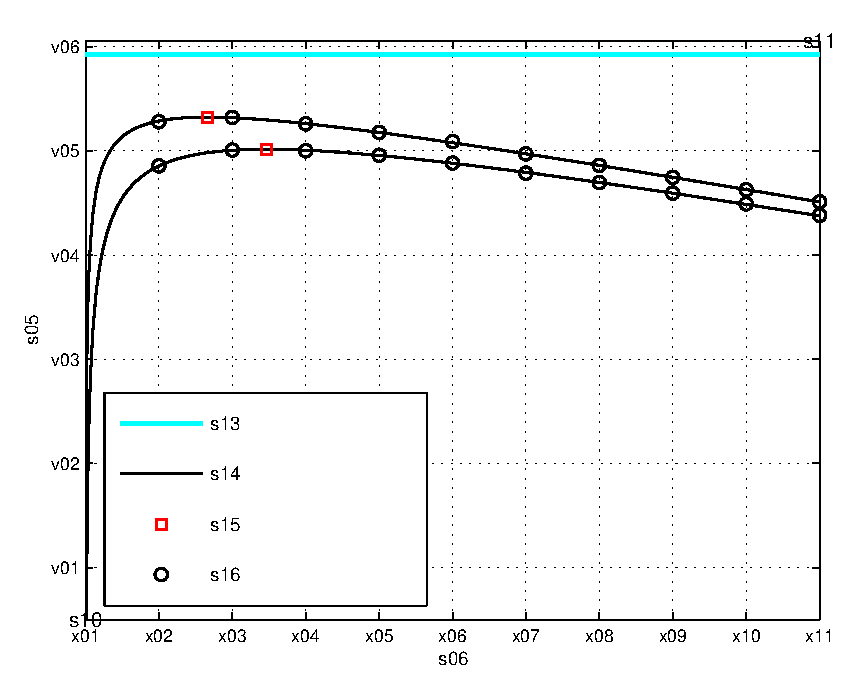
\includegraphics{fig_thr_est_time_tradeoff_AWGN.eps}}%
%\end{psfrags}%
%
% End fig_thr_est_time_tradeoff_AWGN.tex
\end{document}
% See http://www.mathworks.de/matlabcentral/fileexchange/loadFile.do?objectId=4638
% for recent versions of laprint.m.
%
% created by:           LaPrint version 3.16 (13.9.2004)
% created on:           08-Jan-2016 12:22:27
% eps bounding box:     16 cm x 12 cm
% comment:              
%
%\begin{psfrags}%
%\psfragscanon%
%
% text strings:
\psfrag{s05}[b][b]{\fontsize{8.5}{12.75}\fontseries{m}\mathversion{normal}\fontshape{n}\selectfont \color[rgb]{0,0,0}\setlength{\tabcolsep}{0pt}\begin{tabular}{c}$\rs(\tau)$ [bits/sec/Hz]\end{tabular}}%
\psfrag{s06}[t][t]{\fontsize{8.5}{12.75}\fontseries{m}\mathversion{normal}\fontshape{n}\selectfont \color[rgb]{0,0,0}\setlength{\tabcolsep}{0pt}\begin{tabular}{c}$\tau$ [ms]\end{tabular}}%
\psfrag{s10}[][]{\fontsize{10}{15}\fontseries{m}\mathversion{normal}\fontshape{n}\selectfont \color[rgb]{0,0,0}\setlength{\tabcolsep}{0pt}\begin{tabular}{c} \end{tabular}}%
\psfrag{s11}[][]{\fontsize{10}{15}\fontseries{m}\mathversion{normal}\fontshape{n}\selectfont \color[rgb]{0,0,0}\setlength{\tabcolsep}{0pt}\begin{tabular}{c} \end{tabular}}%
\psfrag{s12}[l][l]{\fontsize{8.5}{12.75}\fontseries{m}\mathversion{normal}\fontshape{n}\selectfont \color[rgb]{0,0,0}Simulated}%
\psfrag{s13}[l][l]{\fontsize{8.5}{12.75}\fontseries{m}\mathversion{normal}\fontshape{n}\selectfont \color[rgb]{0,0,0}IM}%
\psfrag{s14}[l][l]{\fontsize{8.5}{12.75}\fontseries{m}\mathversion{normal}\fontshape{n}\selectfont \color[rgb]{0,0,0}EM}%
\psfrag{s15}[l][l]{\fontsize{8.5}{12.75}\fontseries{m}\mathversion{normal}\fontshape{n}\selectfont \color[rgb]{0,0,0}$\trs(\ttau)$}%
\psfrag{s16}[l][l]{\fontsize{8.5}{12.75}\fontseries{m}\mathversion{normal}\fontshape{n}\selectfont \color[rgb]{0,0,0}Simulated}%
%
% axes font properties:
\fontsize{8.5}{12.75}\fontseries{m}\mathversion{normal}%
\fontshape{n}\selectfont%
%
% xticklabels:
\psfrag{x01}[t][t]{0}%
\psfrag{x02}[t][t]{1}%
\psfrag{x03}[t][t]{2}%
\psfrag{x04}[t][t]{3}%
\psfrag{x05}[t][t]{4}%
\psfrag{x06}[t][t]{5}%
\psfrag{x07}[t][t]{6}%
\psfrag{x08}[t][t]{7}%
\psfrag{x09}[t][t]{8}%
\psfrag{x10}[t][t]{9}%
\psfrag{x11}[t][t]{10}%
%
% yticklabels:
\psfrag{v01}[r][r]{1.6}%
\psfrag{v02}[r][r]{1.8}%
\psfrag{v03}[r][r]{2}%
\psfrag{v04}[r][r]{2.2}%
\psfrag{v05}[r][r]{2.4}%
\psfrag{v06}[r][r]{2.6}%
%
% Figure:
%\resizebox{8cm}{!}{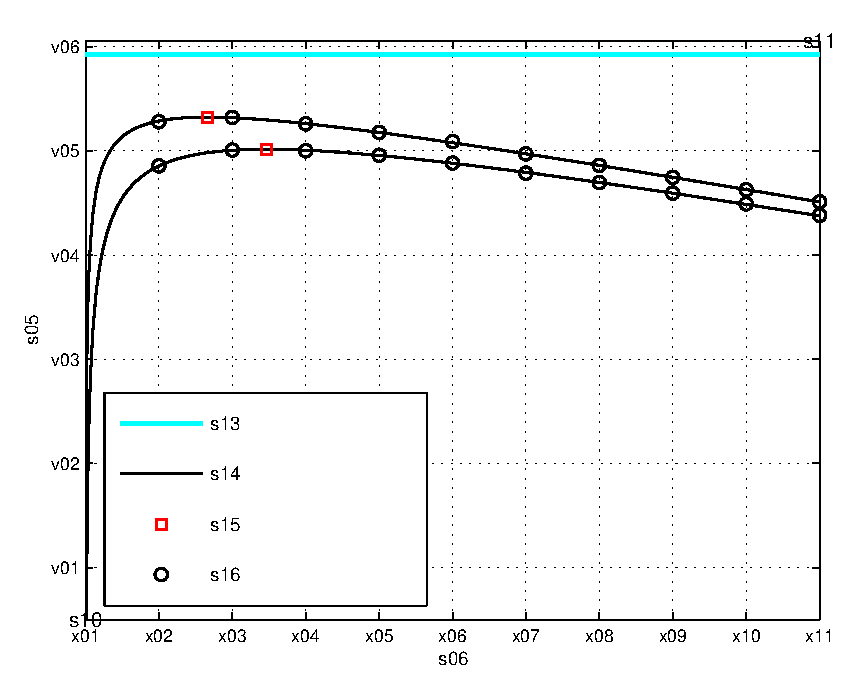
\includegraphics{fig_thr_est_time_tradeoff_AWGN.eps}}%
%\end{psfrags}%
%
% End fig_thr_est_time_tradeoff_AWGN.tex
\end{document}
% See http://www.mathworks.de/matlabcentral/fileexchange/loadFile.do?objectId=4638
% for recent versions of laprint.m.
%
% created by:           LaPrint version 3.16 (13.9.2004)
% created on:           08-Jan-2016 12:22:27
% eps bounding box:     16 cm x 12 cm
% comment:              
%
%\begin{psfrags}%
%\psfragscanon%
%
% text strings:
\psfrag{s05}[b][b]{\fontsize{8.5}{12.75}\fontseries{m}\mathversion{normal}\fontshape{n}\selectfont \color[rgb]{0,0,0}\setlength{\tabcolsep}{0pt}\begin{tabular}{c}$\rs(\tau)$ [bits/sec/Hz]\end{tabular}}%
\psfrag{s06}[t][t]{\fontsize{8.5}{12.75}\fontseries{m}\mathversion{normal}\fontshape{n}\selectfont \color[rgb]{0,0,0}\setlength{\tabcolsep}{0pt}\begin{tabular}{c}$\tau$ [ms]\end{tabular}}%
\psfrag{s10}[][]{\fontsize{10}{15}\fontseries{m}\mathversion{normal}\fontshape{n}\selectfont \color[rgb]{0,0,0}\setlength{\tabcolsep}{0pt}\begin{tabular}{c} \end{tabular}}%
\psfrag{s11}[][]{\fontsize{10}{15}\fontseries{m}\mathversion{normal}\fontshape{n}\selectfont \color[rgb]{0,0,0}\setlength{\tabcolsep}{0pt}\begin{tabular}{c} \end{tabular}}%
\psfrag{s12}[l][l]{\fontsize{8.5}{12.75}\fontseries{m}\mathversion{normal}\fontshape{n}\selectfont \color[rgb]{0,0,0}Simulated}%
\psfrag{s13}[l][l]{\fontsize{8.5}{12.75}\fontseries{m}\mathversion{normal}\fontshape{n}\selectfont \color[rgb]{0,0,0}IM}%
\psfrag{s14}[l][l]{\fontsize{8.5}{12.75}\fontseries{m}\mathversion{normal}\fontshape{n}\selectfont \color[rgb]{0,0,0}EM}%
\psfrag{s15}[l][l]{\fontsize{8.5}{12.75}\fontseries{m}\mathversion{normal}\fontshape{n}\selectfont \color[rgb]{0,0,0}$\trs(\ttau)$}%
\psfrag{s16}[l][l]{\fontsize{8.5}{12.75}\fontseries{m}\mathversion{normal}\fontshape{n}\selectfont \color[rgb]{0,0,0}Simulated}%
%
% axes font properties:
\fontsize{8.5}{12.75}\fontseries{m}\mathversion{normal}%
\fontshape{n}\selectfont%
%
% xticklabels:
\psfrag{x01}[t][t]{0}%
\psfrag{x02}[t][t]{1}%
\psfrag{x03}[t][t]{2}%
\psfrag{x04}[t][t]{3}%
\psfrag{x05}[t][t]{4}%
\psfrag{x06}[t][t]{5}%
\psfrag{x07}[t][t]{6}%
\psfrag{x08}[t][t]{7}%
\psfrag{x09}[t][t]{8}%
\psfrag{x10}[t][t]{9}%
\psfrag{x11}[t][t]{10}%
%
% yticklabels:
\psfrag{v01}[r][r]{1.6}%
\psfrag{v02}[r][r]{1.8}%
\psfrag{v03}[r][r]{2}%
\psfrag{v04}[r][r]{2.2}%
\psfrag{v05}[r][r]{2.4}%
\psfrag{v06}[r][r]{2.6}%
%
% Figure:
%\resizebox{8cm}{!}{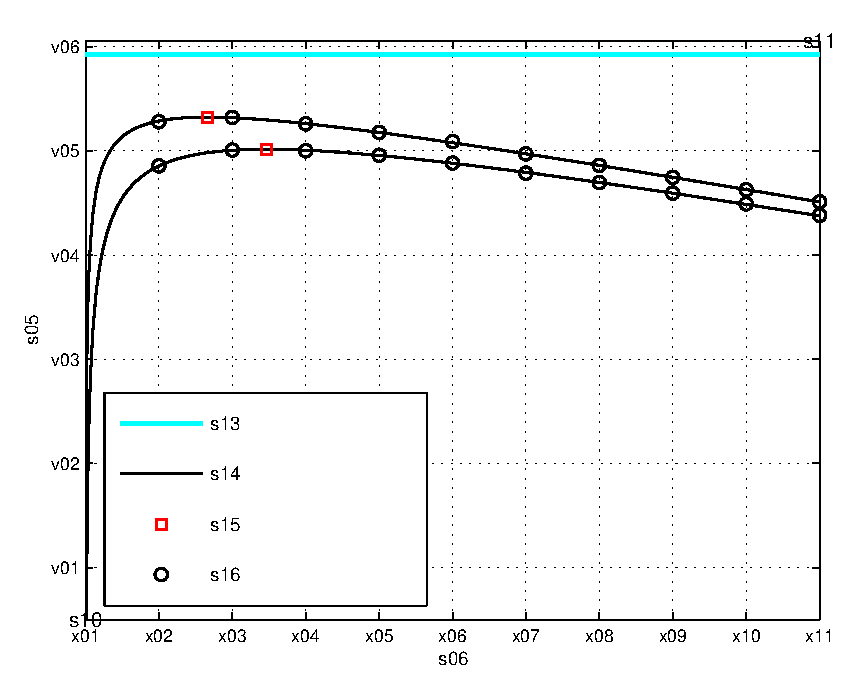
\includegraphics{fig_thr_est_time_tradeoff_AWGN.eps}}%
%\end{psfrags}%
%
% End fig_thr_est_time_tradeoff_AWGN.tex

\centering
\begin{tikzpicture}[scale=1]
\node[anchor=south west,inner sep=0] (image) at (0,0)
{
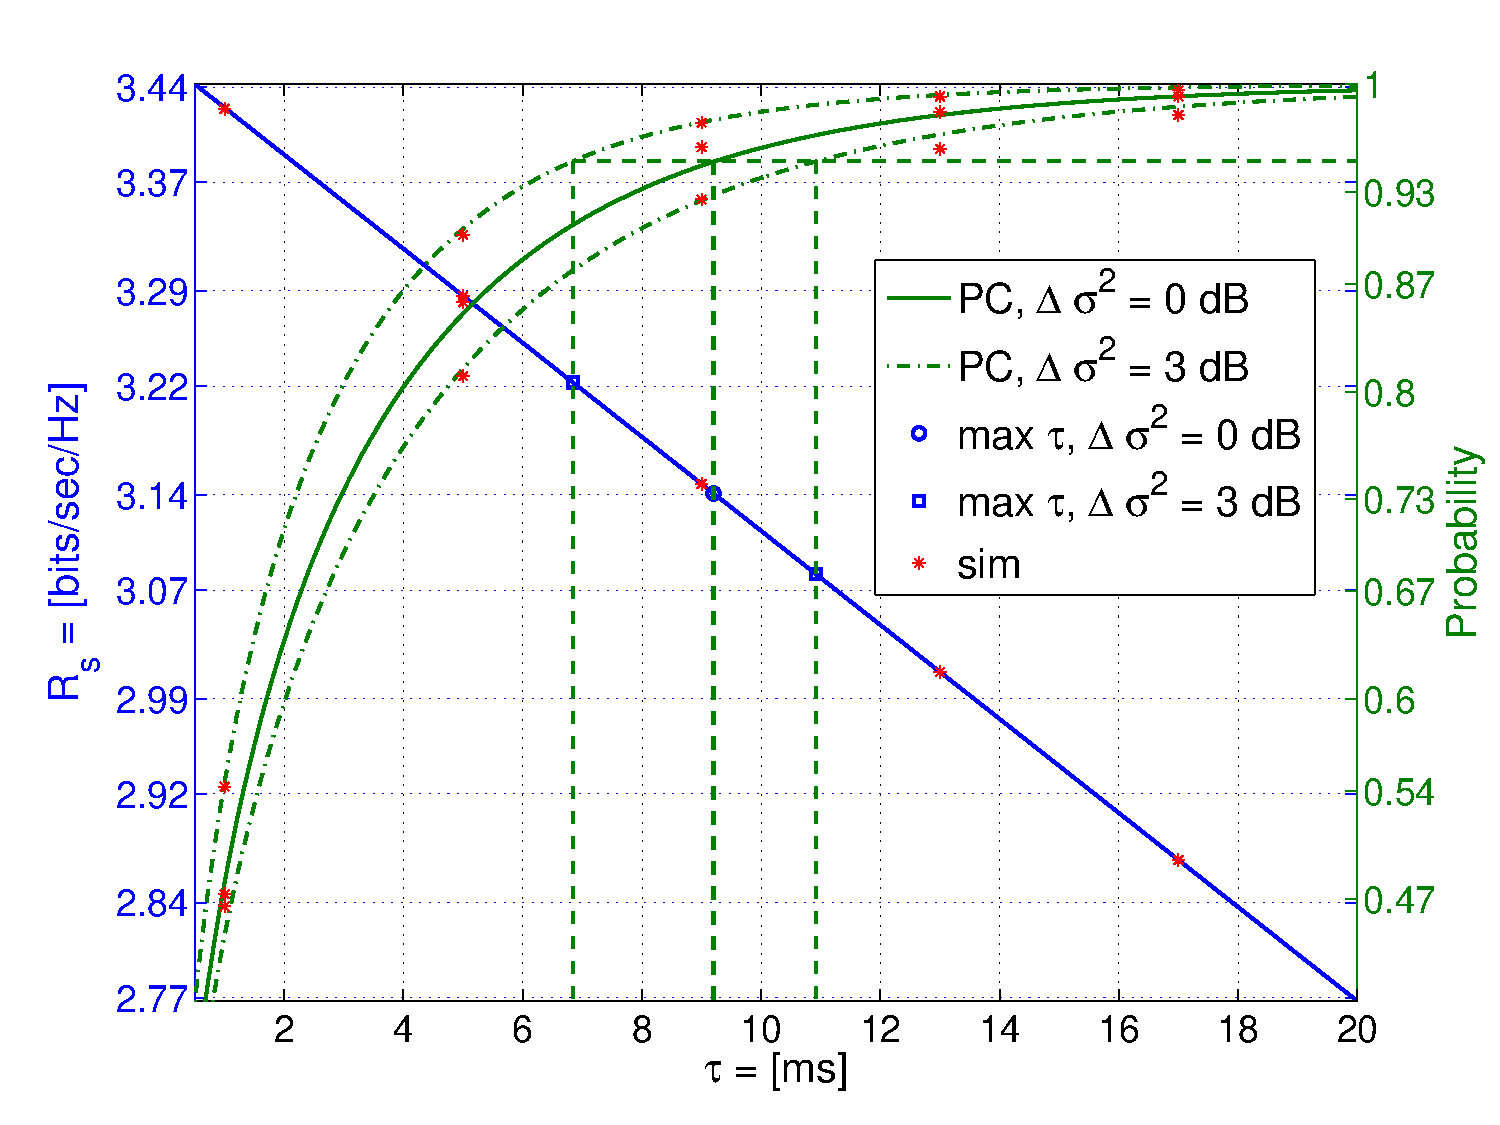
\includegraphics[width= \figscale]{figures/fig_thr_est_time_tradeoff_AWGN}
};
\begin{scope}[x={(image.south east)},y={(image.north west)}]

\draw (0.38,0.78) arc(-130:130:0.005 and 0.015);
\node[draw, fill=gray!10,font=\scriptsize] at (0.39,0.735) {$\opc = 0.01$};

\draw (0.65,0.77) arc(-130:130:0.005 and 0.015);
\node[draw,fill=gray!10,font=\scriptsize] at (0.66,0.838) {$\opc = 0.1$};

%\draw[help lines,xstep=.1,ystep=.1] (0,0) grid (1,1);
%\foreach \x in {0,1,...,9} { \node [anchor=north] at (\x/10,0) {0.\x}; }
%\foreach \y in {0,1,...,9} { \node [anchor=east] at (0,\y/10) {0.\y}; }
\end{scope}
\end{tikzpicture}
\caption{Estimation-throughput tradeoff with $\snrrcvdu = \SI{0}{dB}$, $\opc \in \{0.01, 0.1\}$ and $\pc = \SI{0}{dBm}$.}
\label{fig_US:ETT}
%\vspace{-10mm}
\end{figure}
First, the performance of the proposed framework in context to the deterministic channel is evaluated. \figurename~\ref{fig_US:Cont_snr} considers the variation of $\preg$ (defined in Corollary \ref{cor_US:cor1}) versus $\test$ corresponding to the Ideal Model (IM) and the proposed Estimation Model (EM). It is noticed that the ST controls its transmit power ($\preg$) more severely for low values, consequently affecting the link budget for the access channel. %This concludes that an increase is estimation time compensates for the variations in the system, thereby allowing margin to increase the control power. Furthermore, it is depicted that for $\test \le \SI{0.1}{ms}$, the ST has to control its transmit power ($\preg$), which consequently degrades the link budget for the access channel. 
\figurename~\ref{fig_US:ETT} analyzes the performance of the US in terms of the estimation-throughput tradeoff, refer to Problem \ref{th_US:th1}. %Clearly, by relaxing the $\opc$, an improvement in performance it terms of $\trs$ is observed. 
It can be depicted that the estimation-throughput tradeoff yields a suitable estimation time $\ttest$ that results in an optimum throughput $\trs(\ttest)$. Hereafter, theoretical expressions are considered for the performance analysis with respect to the deterministic channel. In addition, the US operates at the suitable estimation time. 

\captionsetup[subfigure]{position=top}
\begin{figure}[!ht]
\vspace{-5mm}
%% Add psfrag entries
%\vspace{-5mm}
\centering
\subfloat[]{
% This file is generated by the MATLAB m-file laprint.m. It can be included
% into LaTeX documents using the packages graphicx, color and psfrag.
% It is accompanied by a postscript file. A sample LaTeX file is:
%    \documentclass{article}\usepackage{graphicx,color,psfrag}
%    \begin{document}% This file is generated by the MATLAB m-file laprint.m. It can be included
% into LaTeX documents using the packages graphicx, color and psfrag.
% It is accompanied by a postscript file. A sample LaTeX file is:
%    \documentclass{article}\usepackage{graphicx,color,psfrag}
%    \begin{document}% This file is generated by the MATLAB m-file laprint.m. It can be included
% into LaTeX documents using the packages graphicx, color and psfrag.
% It is accompanied by a postscript file. A sample LaTeX file is:
%    \documentclass{article}\usepackage{graphicx,color,psfrag}
%    \begin{document}\input{fig_opt_thr_vs_SNR_AWGN_SI_00}\end{document}
% See http://www.mathworks.de/matlabcentral/fileexchange/loadFile.do?objectId=4638
% for recent versions of laprint.m.
%
% created by:           LaPrint version 3.16 (13.9.2004)
% created on:           08-Jan-2016 18:59:26
% eps bounding box:     16 cm x 12 cm
% comment:              
%
%\begin{psfrags}%
%\psfragscanon%
%
% text strings:
\psfrag{s05}[b][b]{\fontsize{8.5}{12.75}\fontseries{m}\mathversion{normal}\fontshape{n}\selectfont \color[rgb]{0,0,0}\setlength{\tabcolsep}{0pt}\begin{tabular}{c}$\rs(\ttest)$ [bits/sec/Hz]\end{tabular}}%
\psfrag{s06}[t][t]{\fontsize{8.5}{12.75}\fontseries{m}\mathversion{normal}\fontshape{n}\selectfont \color[rgb]{0,0,0}\setlength{\tabcolsep}{0pt}\begin{tabular}{c}$\snrrcvdu$ [dB]\end{tabular}}%
\psfrag{s10}[][]{\fontsize{10}{15}\fontseries{m}\mathversion{normal}\fontshape{n}\selectfont \color[rgb]{0,0,0}\setlength{\tabcolsep}{0pt}\begin{tabular}{c} \end{tabular}}%
\psfrag{s11}[][]{\fontsize{10}{15}\fontseries{m}\mathversion{normal}\fontshape{n}\selectfont \color[rgb]{0,0,0}\setlength{\tabcolsep}{0pt}\begin{tabular}{c} \end{tabular}}%
\psfrag{s12}[l][l]{\fontsize{8.5}{12.75}\fontseries{m}\mathversion{normal}\fontshape{n}\selectfont \color[rgb]{0,0,0}Coro 3}%
\psfrag{s13}[l][l]{\fontsize{8.5}{12.75}\fontseries{m}\mathversion{normal}\fontshape{n}\selectfont \color[rgb]{0,0,0}IM}%
\psfrag{s14}[l][l]{\fontsize{8.5}{12.75}\fontseries{m}\mathversion{normal}\fontshape{n}\selectfont \color[rgb]{0,0,0}EM}%
\psfrag{s15}[l][l]{\fontsize{8.5}{12.75}\fontseries{m}\mathversion{normal}\fontshape{n}\selectfont \color[rgb]{0,0,0}Coro 3}%
%
% axes font properties:
\fontsize{8.5}{12.75}\fontseries{m}\mathversion{normal}%
\fontshape{n}\selectfont%
%
% xticklabels:
\psfrag{x01}[t][t]{-20}%
\psfrag{x02}[t][t]{-15}%
\psfrag{x03}[t][t]{-10}%
\psfrag{x04}[t][t]{-5}%
\psfrag{x05}[t][t]{0}%
\psfrag{x06}[t][t]{5}%
\psfrag{x07}[t][t]{10}%
%
% yticklabels:
\psfrag{v01}[r][r]{0}%
\psfrag{v02}[r][r]{1}%
\psfrag{v03}[r][r]{2}%
\psfrag{v04}[r][r]{3}%
\psfrag{v05}[r][r]{4}%
\psfrag{v06}[r][r]{5}%
\psfrag{v07}[r][r]{6}%
\psfrag{v08}[r][r]{7}%
\psfrag{v09}[r][r]{8}%
\psfrag{v10}[r][r]{9}%
%
% Figure:
%\resizebox{8cm}{!}{\includegraphics{fig_opt_thr_vs_SNR_AWGN_SI_00.eps}}%
%\end{psfrags}%
%
% End fig_opt_thr_vs_SNR_AWGN_SI_00.tex
\end{document}
% See http://www.mathworks.de/matlabcentral/fileexchange/loadFile.do?objectId=4638
% for recent versions of laprint.m.
%
% created by:           LaPrint version 3.16 (13.9.2004)
% created on:           08-Jan-2016 18:59:26
% eps bounding box:     16 cm x 12 cm
% comment:              
%
%\begin{psfrags}%
%\psfragscanon%
%
% text strings:
\psfrag{s05}[b][b]{\fontsize{8.5}{12.75}\fontseries{m}\mathversion{normal}\fontshape{n}\selectfont \color[rgb]{0,0,0}\setlength{\tabcolsep}{0pt}\begin{tabular}{c}$\rs(\ttest)$ [bits/sec/Hz]\end{tabular}}%
\psfrag{s06}[t][t]{\fontsize{8.5}{12.75}\fontseries{m}\mathversion{normal}\fontshape{n}\selectfont \color[rgb]{0,0,0}\setlength{\tabcolsep}{0pt}\begin{tabular}{c}$\snrrcvdu$ [dB]\end{tabular}}%
\psfrag{s10}[][]{\fontsize{10}{15}\fontseries{m}\mathversion{normal}\fontshape{n}\selectfont \color[rgb]{0,0,0}\setlength{\tabcolsep}{0pt}\begin{tabular}{c} \end{tabular}}%
\psfrag{s11}[][]{\fontsize{10}{15}\fontseries{m}\mathversion{normal}\fontshape{n}\selectfont \color[rgb]{0,0,0}\setlength{\tabcolsep}{0pt}\begin{tabular}{c} \end{tabular}}%
\psfrag{s12}[l][l]{\fontsize{8.5}{12.75}\fontseries{m}\mathversion{normal}\fontshape{n}\selectfont \color[rgb]{0,0,0}Coro 3}%
\psfrag{s13}[l][l]{\fontsize{8.5}{12.75}\fontseries{m}\mathversion{normal}\fontshape{n}\selectfont \color[rgb]{0,0,0}IM}%
\psfrag{s14}[l][l]{\fontsize{8.5}{12.75}\fontseries{m}\mathversion{normal}\fontshape{n}\selectfont \color[rgb]{0,0,0}EM}%
\psfrag{s15}[l][l]{\fontsize{8.5}{12.75}\fontseries{m}\mathversion{normal}\fontshape{n}\selectfont \color[rgb]{0,0,0}Coro 3}%
%
% axes font properties:
\fontsize{8.5}{12.75}\fontseries{m}\mathversion{normal}%
\fontshape{n}\selectfont%
%
% xticklabels:
\psfrag{x01}[t][t]{-20}%
\psfrag{x02}[t][t]{-15}%
\psfrag{x03}[t][t]{-10}%
\psfrag{x04}[t][t]{-5}%
\psfrag{x05}[t][t]{0}%
\psfrag{x06}[t][t]{5}%
\psfrag{x07}[t][t]{10}%
%
% yticklabels:
\psfrag{v01}[r][r]{0}%
\psfrag{v02}[r][r]{1}%
\psfrag{v03}[r][r]{2}%
\psfrag{v04}[r][r]{3}%
\psfrag{v05}[r][r]{4}%
\psfrag{v06}[r][r]{5}%
\psfrag{v07}[r][r]{6}%
\psfrag{v08}[r][r]{7}%
\psfrag{v09}[r][r]{8}%
\psfrag{v10}[r][r]{9}%
%
% Figure:
%\resizebox{8cm}{!}{\includegraphics{fig_opt_thr_vs_SNR_AWGN_SI_00.eps}}%
%\end{psfrags}%
%
% End fig_opt_thr_vs_SNR_AWGN_SI_00.tex
\end{document}
% See http://www.mathworks.de/matlabcentral/fileexchange/loadFile.do?objectId=4638
% for recent versions of laprint.m.
%
% created by:           LaPrint version 3.16 (13.9.2004)
% created on:           08-Jan-2016 18:59:26
% eps bounding box:     16 cm x 12 cm
% comment:              
%
%\begin{psfrags}%
%\psfragscanon%
%
% text strings:
\psfrag{s05}[b][b]{\fontsize{8.5}{12.75}\fontseries{m}\mathversion{normal}\fontshape{n}\selectfont \color[rgb]{0,0,0}\setlength{\tabcolsep}{0pt}\begin{tabular}{c}$\rs(\ttest)$ [bits/sec/Hz]\end{tabular}}%
\psfrag{s06}[t][t]{\fontsize{8.5}{12.75}\fontseries{m}\mathversion{normal}\fontshape{n}\selectfont \color[rgb]{0,0,0}\setlength{\tabcolsep}{0pt}\begin{tabular}{c}$\snrrcvdu$ [dB]\end{tabular}}%
\psfrag{s10}[][]{\fontsize{10}{15}\fontseries{m}\mathversion{normal}\fontshape{n}\selectfont \color[rgb]{0,0,0}\setlength{\tabcolsep}{0pt}\begin{tabular}{c} \end{tabular}}%
\psfrag{s11}[][]{\fontsize{10}{15}\fontseries{m}\mathversion{normal}\fontshape{n}\selectfont \color[rgb]{0,0,0}\setlength{\tabcolsep}{0pt}\begin{tabular}{c} \end{tabular}}%
\psfrag{s12}[l][l]{\fontsize{8.5}{12.75}\fontseries{m}\mathversion{normal}\fontshape{n}\selectfont \color[rgb]{0,0,0}Coro 3}%
\psfrag{s13}[l][l]{\fontsize{8.5}{12.75}\fontseries{m}\mathversion{normal}\fontshape{n}\selectfont \color[rgb]{0,0,0}IM}%
\psfrag{s14}[l][l]{\fontsize{8.5}{12.75}\fontseries{m}\mathversion{normal}\fontshape{n}\selectfont \color[rgb]{0,0,0}EM}%
\psfrag{s15}[l][l]{\fontsize{8.5}{12.75}\fontseries{m}\mathversion{normal}\fontshape{n}\selectfont \color[rgb]{0,0,0}Coro 3}%
%
% axes font properties:
\fontsize{8.5}{12.75}\fontseries{m}\mathversion{normal}%
\fontshape{n}\selectfont%
%
% xticklabels:
\psfrag{x01}[t][t]{-20}%
\psfrag{x02}[t][t]{-15}%
\psfrag{x03}[t][t]{-10}%
\psfrag{x04}[t][t]{-5}%
\psfrag{x05}[t][t]{0}%
\psfrag{x06}[t][t]{5}%
\psfrag{x07}[t][t]{10}%
%
% yticklabels:
\psfrag{v01}[r][r]{0}%
\psfrag{v02}[r][r]{1}%
\psfrag{v03}[r][r]{2}%
\psfrag{v04}[r][r]{3}%
\psfrag{v05}[r][r]{4}%
\psfrag{v06}[r][r]{5}%
\psfrag{v07}[r][r]{6}%
\psfrag{v08}[r][r]{7}%
\psfrag{v09}[r][r]{8}%
\psfrag{v10}[r][r]{9}%
%
% Figure:
%\resizebox{8cm}{!}{\includegraphics{fig_opt_thr_vs_SNR_AWGN_SI_00.eps}}%
%\end{psfrags}%
%
% End fig_opt_thr_vs_SNR_AWGN_SI_00.tex

\centering
\begin{tikzpicture}[scale=1]
\node[anchor=south west,inner sep=0] (image) at (0,0)
{
	\includegraphics[width= \figscale]{figures/fig_opt_thr_vs_SNR_AWGN_SI_00}
};
\begin{scope}[x={(image.south east)},y={(image.north west)}]

\draw (0.225,0.615) arc(-160:160:0.01 and 0.03);
\node[draw, fill=gray!10, font=\scriptsize] (text1) at (0.7,0.725) {$\pc = \SI{00}{dBm}$};
\draw (0.275,0.33) arc(-160:160:0.01 and 0.03);
\node[draw, fill=gray!10, font=\scriptsize] (text2) at (0.75,0.44) {$\pc = \SI{-10}{dBm}$};
%\draw (0.63,0.66) arc(-150:150:0.016 and 0.048);
\draw[black, ->] (text1.west) -- (0.245,0.635);
%\draw (0.63,0.59) arc(-160:160:0.01 and 0.03);
\draw[black, ->] (text2.west) -- (0.295,0.35);


\draw (0.27,0.225) arc(-160:160:0.01 and 0.03);
\draw[black,thick,<->] (0.084,0.25) --  node[above, font=\scriptsize] {Power-limited} (0.367,0.25);
\draw[black,thick,<->] (0.084,0.22) --  (0.667,0.22);

\draw (0.7,0.105) arc(-160:160:0.01 and 0.03);
\draw[black,thick,<->] (0.37,0.13) --  node[above, font=\scriptsize] {Interference-limited} (0.965,0.13);
\draw[black,thick,<->] (0.67,0.10) --  (0.965,0.10);

%\draw[help lines,xstep=.1,ystep=.1] (0,0) grid (1,1);
%\foreach \x in {0,1,...,9} { \node [anchor=north] at (\x/10,0) {0.\x}; }
%\foreach \y in {0,1,...,9} { \node [anchor=east] at (0,\y/10) {0.\y}; }
\end{scope}
\end{tikzpicture}
\label{fig_US:optT_snr_a}
}
\hfil
\subfloat[]{
% This file is generated by the MATLAB m-file laprint.m. It can be included
% into LaTeX documents using the packages graphicx, color and psfrag.
% It is accompanied by a postscript file. A sample LaTeX file is:
%    \documentclass{article}\usepackage{graphicx,color,psfrag}
%    \begin{document}% This file is generated by the MATLAB m-file laprint.m. It can be included
% into LaTeX documents using the packages graphicx, color and psfrag.
% It is accompanied by a postscript file. A sample LaTeX file is:
%    \documentclass{article}\usepackage{graphicx,color,psfrag}
%    \begin{document}% This file is generated by the MATLAB m-file laprint.m. It can be included
% into LaTeX documents using the packages graphicx, color and psfrag.
% It is accompanied by a postscript file. A sample LaTeX file is:
%    \documentclass{article}\usepackage{graphicx,color,psfrag}
%    \begin{document}\input{fig_opt_thr_vs_SNR_AWGN_SI_10}\end{document}
% See http://www.mathworks.de/matlabcentral/fileexchange/loadFile.do?objectId=4638
% for recent versions of laprint.m.
%
% created by:           LaPrint version 3.16 (13.9.2004)
% created on:           08-Jan-2016 18:59:27
% eps bounding box:     16 cm x 12 cm
% comment:              
%
%\begin{psfrags}%
%\psfragscanon%
%
% text strings:
\psfrag{s05}[b][b]{\fontsize{8.5}{12.75}\fontseries{m}\mathversion{normal}\fontshape{n}\selectfont \color[rgb]{0,0,0}\setlength{\tabcolsep}{0pt}\begin{tabular}{c}$\rs(\ttest)$ [bits/sec/Hz]\end{tabular}}%
\psfrag{s06}[t][t]{\fontsize{8.5}{12.75}\fontseries{m}\mathversion{normal}\fontshape{n}\selectfont \color[rgb]{0,0,0}\setlength{\tabcolsep}{0pt}\begin{tabular}{c}$\snrrcvdu$ [dB]\end{tabular}}%
\psfrag{s10}[][]{\fontsize{10}{15}\fontseries{m}\mathversion{normal}\fontshape{n}\selectfont \color[rgb]{0,0,0}\setlength{\tabcolsep}{0pt}\begin{tabular}{c} \end{tabular}}%
\psfrag{s11}[][]{\fontsize{10}{15}\fontseries{m}\mathversion{normal}\fontshape{n}\selectfont \color[rgb]{0,0,0}\setlength{\tabcolsep}{0pt}\begin{tabular}{c} \end{tabular}}%
\psfrag{s12}[l][l]{\fontsize{8.5}{12.75}\fontseries{m}\mathversion{normal}\fontshape{n}\selectfont \color[rgb]{0,0,0}Coro 3}%
\psfrag{s13}[l][l]{\fontsize{8.5}{12.75}\fontseries{m}\mathversion{normal}\fontshape{n}\selectfont \color[rgb]{0,0,0}IM}%
\psfrag{s14}[l][l]{\fontsize{8.5}{12.75}\fontseries{m}\mathversion{normal}\fontshape{n}\selectfont \color[rgb]{0,0,0}EM}%
\psfrag{s15}[l][l]{\fontsize{8.5}{12.75}\fontseries{m}\mathversion{normal}\fontshape{n}\selectfont \color[rgb]{0,0,0}Coro 3}%
%
% axes font properties:
\fontsize{8.5}{12.75}\fontseries{m}\mathversion{normal}%
\fontshape{n}\selectfont%
%
% xticklabels:
\psfrag{x01}[t][t]{-20}%
\psfrag{x02}[t][t]{-15}%
\psfrag{x03}[t][t]{-10}%
\psfrag{x04}[t][t]{-5}%
\psfrag{x05}[t][t]{0}%
\psfrag{x06}[t][t]{5}%
\psfrag{x07}[t][t]{10}%
%
% yticklabels:
\psfrag{v01}[r][r]{0}%
\psfrag{v02}[r][r]{1}%
\psfrag{v03}[r][r]{2}%
\psfrag{v04}[r][r]{3}%
\psfrag{v05}[r][r]{4}%
\psfrag{v06}[r][r]{5}%
\psfrag{v07}[r][r]{6}%
%
% Figure:
%\resizebox{8cm}{!}{\includegraphics{fig_opt_thr_vs_SNR_AWGN_SI_10.eps}}%
%\end{psfrags}%
%
% End fig_opt_thr_vs_SNR_AWGN_SI_10.tex
\end{document}
% See http://www.mathworks.de/matlabcentral/fileexchange/loadFile.do?objectId=4638
% for recent versions of laprint.m.
%
% created by:           LaPrint version 3.16 (13.9.2004)
% created on:           08-Jan-2016 18:59:27
% eps bounding box:     16 cm x 12 cm
% comment:              
%
%\begin{psfrags}%
%\psfragscanon%
%
% text strings:
\psfrag{s05}[b][b]{\fontsize{8.5}{12.75}\fontseries{m}\mathversion{normal}\fontshape{n}\selectfont \color[rgb]{0,0,0}\setlength{\tabcolsep}{0pt}\begin{tabular}{c}$\rs(\ttest)$ [bits/sec/Hz]\end{tabular}}%
\psfrag{s06}[t][t]{\fontsize{8.5}{12.75}\fontseries{m}\mathversion{normal}\fontshape{n}\selectfont \color[rgb]{0,0,0}\setlength{\tabcolsep}{0pt}\begin{tabular}{c}$\snrrcvdu$ [dB]\end{tabular}}%
\psfrag{s10}[][]{\fontsize{10}{15}\fontseries{m}\mathversion{normal}\fontshape{n}\selectfont \color[rgb]{0,0,0}\setlength{\tabcolsep}{0pt}\begin{tabular}{c} \end{tabular}}%
\psfrag{s11}[][]{\fontsize{10}{15}\fontseries{m}\mathversion{normal}\fontshape{n}\selectfont \color[rgb]{0,0,0}\setlength{\tabcolsep}{0pt}\begin{tabular}{c} \end{tabular}}%
\psfrag{s12}[l][l]{\fontsize{8.5}{12.75}\fontseries{m}\mathversion{normal}\fontshape{n}\selectfont \color[rgb]{0,0,0}Coro 3}%
\psfrag{s13}[l][l]{\fontsize{8.5}{12.75}\fontseries{m}\mathversion{normal}\fontshape{n}\selectfont \color[rgb]{0,0,0}IM}%
\psfrag{s14}[l][l]{\fontsize{8.5}{12.75}\fontseries{m}\mathversion{normal}\fontshape{n}\selectfont \color[rgb]{0,0,0}EM}%
\psfrag{s15}[l][l]{\fontsize{8.5}{12.75}\fontseries{m}\mathversion{normal}\fontshape{n}\selectfont \color[rgb]{0,0,0}Coro 3}%
%
% axes font properties:
\fontsize{8.5}{12.75}\fontseries{m}\mathversion{normal}%
\fontshape{n}\selectfont%
%
% xticklabels:
\psfrag{x01}[t][t]{-20}%
\psfrag{x02}[t][t]{-15}%
\psfrag{x03}[t][t]{-10}%
\psfrag{x04}[t][t]{-5}%
\psfrag{x05}[t][t]{0}%
\psfrag{x06}[t][t]{5}%
\psfrag{x07}[t][t]{10}%
%
% yticklabels:
\psfrag{v01}[r][r]{0}%
\psfrag{v02}[r][r]{1}%
\psfrag{v03}[r][r]{2}%
\psfrag{v04}[r][r]{3}%
\psfrag{v05}[r][r]{4}%
\psfrag{v06}[r][r]{5}%
\psfrag{v07}[r][r]{6}%
%
% Figure:
%\resizebox{8cm}{!}{\includegraphics{fig_opt_thr_vs_SNR_AWGN_SI_10.eps}}%
%\end{psfrags}%
%
% End fig_opt_thr_vs_SNR_AWGN_SI_10.tex
\end{document}
% See http://www.mathworks.de/matlabcentral/fileexchange/loadFile.do?objectId=4638
% for recent versions of laprint.m.
%
% created by:           LaPrint version 3.16 (13.9.2004)
% created on:           08-Jan-2016 18:59:27
% eps bounding box:     16 cm x 12 cm
% comment:              
%
%\begin{psfrags}%
%\psfragscanon%
%
% text strings:
\psfrag{s05}[b][b]{\fontsize{8.5}{12.75}\fontseries{m}\mathversion{normal}\fontshape{n}\selectfont \color[rgb]{0,0,0}\setlength{\tabcolsep}{0pt}\begin{tabular}{c}$\rs(\ttest)$ [bits/sec/Hz]\end{tabular}}%
\psfrag{s06}[t][t]{\fontsize{8.5}{12.75}\fontseries{m}\mathversion{normal}\fontshape{n}\selectfont \color[rgb]{0,0,0}\setlength{\tabcolsep}{0pt}\begin{tabular}{c}$\snrrcvdu$ [dB]\end{tabular}}%
\psfrag{s10}[][]{\fontsize{10}{15}\fontseries{m}\mathversion{normal}\fontshape{n}\selectfont \color[rgb]{0,0,0}\setlength{\tabcolsep}{0pt}\begin{tabular}{c} \end{tabular}}%
\psfrag{s11}[][]{\fontsize{10}{15}\fontseries{m}\mathversion{normal}\fontshape{n}\selectfont \color[rgb]{0,0,0}\setlength{\tabcolsep}{0pt}\begin{tabular}{c} \end{tabular}}%
\psfrag{s12}[l][l]{\fontsize{8.5}{12.75}\fontseries{m}\mathversion{normal}\fontshape{n}\selectfont \color[rgb]{0,0,0}Coro 3}%
\psfrag{s13}[l][l]{\fontsize{8.5}{12.75}\fontseries{m}\mathversion{normal}\fontshape{n}\selectfont \color[rgb]{0,0,0}IM}%
\psfrag{s14}[l][l]{\fontsize{8.5}{12.75}\fontseries{m}\mathversion{normal}\fontshape{n}\selectfont \color[rgb]{0,0,0}EM}%
\psfrag{s15}[l][l]{\fontsize{8.5}{12.75}\fontseries{m}\mathversion{normal}\fontshape{n}\selectfont \color[rgb]{0,0,0}Coro 3}%
%
% axes font properties:
\fontsize{8.5}{12.75}\fontseries{m}\mathversion{normal}%
\fontshape{n}\selectfont%
%
% xticklabels:
\psfrag{x01}[t][t]{-20}%
\psfrag{x02}[t][t]{-15}%
\psfrag{x03}[t][t]{-10}%
\psfrag{x04}[t][t]{-5}%
\psfrag{x05}[t][t]{0}%
\psfrag{x06}[t][t]{5}%
\psfrag{x07}[t][t]{10}%
%
% yticklabels:
\psfrag{v01}[r][r]{0}%
\psfrag{v02}[r][r]{1}%
\psfrag{v03}[r][r]{2}%
\psfrag{v04}[r][r]{3}%
\psfrag{v05}[r][r]{4}%
\psfrag{v06}[r][r]{5}%
\psfrag{v07}[r][r]{6}%
%
% Figure:
%\resizebox{8cm}{!}{\includegraphics{fig_opt_thr_vs_SNR_AWGN_SI_10.eps}}%
%\end{psfrags}%
%
% End fig_opt_thr_vs_SNR_AWGN_SI_10.tex

\centering
\begin{tikzpicture}[scale=1]
\node[anchor=south west,inner sep=0] (image) at (0,0)
{
	\includegraphics[width= \figscale]{figures/fig_opt_thr_vs_SNR_AWGN_SI_10}
};
\begin{scope}[x={(image.south east)},y={(image.north west)}]

\draw (0.225,0.51) arc(-160:160:0.01 and 0.03);
\node[draw, fill=gray!10, font=\scriptsize] (text1) at (0.7,0.66) {$\pc = \SI{00}{dBm}$};
\draw (0.275,0.2) arc(-160:160:0.01 and 0.03);
\node[draw, fill=gray!10, font=\scriptsize] (text2) at (0.75,0.35) {$\pc = \SI{-10}{dBm}$};
%\draw (0.63,0.66) arc(-150:150:0.016 and 0.048);
\draw[black, ->] (text1.west) -- (0.245,0.53);
%\draw (0.63,0.58) arc(-160:160:0.01 and 0.03);
\draw[black, ->] (text2.west) -- (0.295,0.22);

%\draw[help lines,xstep=.1,ystep=.1] (0,0) grid (1,1);
%\foreach \x in {0,1,...,9} { \node [anchor=north] at (\x/10,0) {0.\x}; }
%\foreach \y in {0,1,...,9} { \node [anchor=east] at (0,\y/10) {0.\y}; }
\end{scope}
\end{tikzpicture}
\label{fig_US:optT_snr_b}
}
%\vspace{4mm}
\caption{$\rs(\ttest)$ versus $\snrrcvdu$ with $\opc = 0.1$ and $\pc \in \{-10, 0\} \SI{}{dBm}$ for (a) $\pgpt = \SI{-100}{dBm}$ and (b) $\pgpt = \SI{-90}{dBm}$, which translate to an interference power (from the PT) to noise ratio of (a) $\SI{0}{dB}$ and (b) $\SI{10}{dB}$, respectively, at the SR.}
\label{fig_US:optT_snr}
%\vspace{-10mm}
\end{figure}
To procure further insights, it is necessary to consider the variation of $\trs(\ttest)$ with $\snrrcvdu$ for different choices of the secondary interference at the SR (regulated using $\pgpt \in \{-90, -100\} \SI{}{dBm}$), as depicted in \figurename~\ref{fig_US:optT_snr}. Here, the power-limited and the interference-limited regimes classified in Corollary \ref{cor_US:cor2} are mapped onto the achievable secondary throughput, refer to \figurename~\ref{fig_US:optT_snr_a}. It is observed that due to the employed transmit power constraint, $\trs(\ttest)$ gets saturated below a certain $\snrrcvdu$, thereby limiting the performance of the US. It is worthy to note that this saturation is due to the operation of the US inside the power-limited regime, which is restricted due to the existence of the performance bound. Upon increasing $\pc$ from $\SI{-10}{dB}$ to $\SI{0}{dB}$, the point where saturation is achieved shifts to a lower $\snrrcvdu$. This is due to the fact that higher $\pc$ extends the interference-limited regime to a lower $\snrrcvdu$. In other words, this reveals the fact that the higher controlled power allows the secondary system to operate at lower values of $\snrrcvdu$, hence, beneficial in terms of achievable throughput. Particularly for $\pc = \SI{-10}{dBm}$, a severe performance loss indicated by the margin between the IM and the EM is witnessed by the US for $\snrrcvdu \le \SI{-2}{dB}$. This signifies that the consideration of the maximum transmit power of the ST is essential while designing the system. Besides this, \figurename~\ref{fig_US:optT_snr} depicts the performance of the USs with no power control, proposed in Corollary \ref{cor_US:cor2}. As indicated in \figurename~\ref{fig_US:or}, beyond a certain $\snrrcvdu = \snrrcvdu^*$, the USs with no power control delivers no throughput. In order to avoid such situations, the US can exercise power control in order to deliver non-zero throughput, thereby allowing the USs to operate in the interference-limited regime. 
%%%%%%%%%%%%%%%%%%%%%%%%%%%%%%%%%%%%%%%%%%%%%%%%%%%%%%%%%%%%%%%%%%%%%%%%%%%%%%%%%%%%%%%%%
\subsection{Random Channel} 
%%%%%%%%%%%%%%%%%%%%%%%%%%%%%%%%%%%%%%%%%%%%%%%%%%%%%%%%%%%%%%%%%%%%%%%%%%%%%%%%%%%%%%%%%

\begin{figure}[!t]
\vspace{-4mm}
%% Add psfrag entries
% This file is generated by the MATLAB m-file laprint.m. It can be included
% into LaTeX documents using the packages graphicx, color and psfrag.
% It is accompanied by a postscript file. A sample LaTeX file is:
%    \documentclass{article}\usepackage{graphicx,color,psfrag}
%    \begin{document}% This file is generated by the MATLAB m-file laprint.m. It can be included
% into LaTeX documents using the packages graphicx, color and psfrag.
% It is accompanied by a postscript file. A sample LaTeX file is:
%    \documentclass{article}\usepackage{graphicx,color,psfrag}
%    \begin{document}% This file is generated by the MATLAB m-file laprint.m. It can be included
% into LaTeX documents using the packages graphicx, color and psfrag.
% It is accompanied by a postscript file. A sample LaTeX file is:
%    \documentclass{article}\usepackage{graphicx,color,psfrag}
%    \begin{document}\input{fig_Preg_est_time_fading}\end{document}
% See http://www.mathworks.de/matlabcentral/fileexchange/loadFile.do?objectId=4638
% for recent versions of laprint.m.
%
% created by:           LaPrint version 3.16 (13.9.2004)
% created on:           06-Jan-2016 11:38:28
% eps bounding box:     16 cm x 12 cm
% comment:              
%
%\begin{psfrags}%
%\psfragscanon%
%
% text strings:
\psfrag{s05}[b][b]{\fontsize{8.5}{12.75}\fontseries{m}\mathversion{normal}\fontshape{n}\selectfont \color[rgb]{0,0,0}\setlength{\tabcolsep}{0pt}\begin{tabular}{c}$\preg$ [dBm]\end{tabular}}%
\psfrag{s06}[t][t]{\fontsize{8.5}{12.75}\fontseries{m}\mathversion{normal}\fontshape{n}\selectfont \color[rgb]{0,0,0}\setlength{\tabcolsep}{0pt}\begin{tabular}{c}$\test$ [ms]\end{tabular}}%
\psfrag{s10}[][]{\fontsize{10}{15}\fontseries{m}\mathversion{normal}\fontshape{n}\selectfont \color[rgb]{0,0,0}\setlength{\tabcolsep}{0pt}\begin{tabular}{c} \end{tabular}}%
\psfrag{s11}[][]{\fontsize{10}{15}\fontseries{m}\mathversion{normal}\fontshape{n}\selectfont \color[rgb]{0,0,0}\setlength{\tabcolsep}{0pt}\begin{tabular}{c} \end{tabular}}%
\psfrag{s12}[l][l]{\fontsize{8.5}{12.75}\fontseries{m}\mathversion{normal}\fontshape{n}\selectfont \color[rgb]{0,0,0}Simulated}%
\psfrag{s13}[l][l]{\fontsize{8.5}{12.75}\fontseries{m}\mathversion{normal}\fontshape{n}\selectfont \color[rgb]{0,0,0}IM}%
\psfrag{s14}[l][l]{\fontsize{8.5}{12.75}\fontseries{m}\mathversion{normal}\fontshape{n}\selectfont \color[rgb]{0,0,0}EM}%
\psfrag{s15}[l][l]{\fontsize{8.5}{12.75}\fontseries{m}\mathversion{normal}\fontshape{n}\selectfont \color[rgb]{0,0,0}Simulated}%
%
% axes font properties:
\fontsize{8.5}{12.75}\fontseries{m}\mathversion{normal}%
\fontshape{n}\selectfont%
%
% xticklabels:
\psfrag{x01}[t][t]{$10^{-2}$}%
\psfrag{x02}[t][t]{$10^{-1}$}%
\psfrag{x03}[t][t]{$10^{0}$}%
\psfrag{x04}[t][t]{$10^{1}$}%
%
% yticklabels:
\psfrag{v01}[r][r]{-14}%
\psfrag{v02}[r][r]{-13}%
\psfrag{v03}[r][r]{-12}%
%
% Figure:
%\resizebox{8cm}{!}{\includegraphics{fig_Preg_est_time_fading.eps}}%
%\end{psfrags}%
%
% End fig_Preg_est_time_fading.tex
\end{document}
% See http://www.mathworks.de/matlabcentral/fileexchange/loadFile.do?objectId=4638
% for recent versions of laprint.m.
%
% created by:           LaPrint version 3.16 (13.9.2004)
% created on:           06-Jan-2016 11:38:28
% eps bounding box:     16 cm x 12 cm
% comment:              
%
%\begin{psfrags}%
%\psfragscanon%
%
% text strings:
\psfrag{s05}[b][b]{\fontsize{8.5}{12.75}\fontseries{m}\mathversion{normal}\fontshape{n}\selectfont \color[rgb]{0,0,0}\setlength{\tabcolsep}{0pt}\begin{tabular}{c}$\preg$ [dBm]\end{tabular}}%
\psfrag{s06}[t][t]{\fontsize{8.5}{12.75}\fontseries{m}\mathversion{normal}\fontshape{n}\selectfont \color[rgb]{0,0,0}\setlength{\tabcolsep}{0pt}\begin{tabular}{c}$\test$ [ms]\end{tabular}}%
\psfrag{s10}[][]{\fontsize{10}{15}\fontseries{m}\mathversion{normal}\fontshape{n}\selectfont \color[rgb]{0,0,0}\setlength{\tabcolsep}{0pt}\begin{tabular}{c} \end{tabular}}%
\psfrag{s11}[][]{\fontsize{10}{15}\fontseries{m}\mathversion{normal}\fontshape{n}\selectfont \color[rgb]{0,0,0}\setlength{\tabcolsep}{0pt}\begin{tabular}{c} \end{tabular}}%
\psfrag{s12}[l][l]{\fontsize{8.5}{12.75}\fontseries{m}\mathversion{normal}\fontshape{n}\selectfont \color[rgb]{0,0,0}Simulated}%
\psfrag{s13}[l][l]{\fontsize{8.5}{12.75}\fontseries{m}\mathversion{normal}\fontshape{n}\selectfont \color[rgb]{0,0,0}IM}%
\psfrag{s14}[l][l]{\fontsize{8.5}{12.75}\fontseries{m}\mathversion{normal}\fontshape{n}\selectfont \color[rgb]{0,0,0}EM}%
\psfrag{s15}[l][l]{\fontsize{8.5}{12.75}\fontseries{m}\mathversion{normal}\fontshape{n}\selectfont \color[rgb]{0,0,0}Simulated}%
%
% axes font properties:
\fontsize{8.5}{12.75}\fontseries{m}\mathversion{normal}%
\fontshape{n}\selectfont%
%
% xticklabels:
\psfrag{x01}[t][t]{$10^{-2}$}%
\psfrag{x02}[t][t]{$10^{-1}$}%
\psfrag{x03}[t][t]{$10^{0}$}%
\psfrag{x04}[t][t]{$10^{1}$}%
%
% yticklabels:
\psfrag{v01}[r][r]{-14}%
\psfrag{v02}[r][r]{-13}%
\psfrag{v03}[r][r]{-12}%
%
% Figure:
%\resizebox{8cm}{!}{\includegraphics{fig_Preg_est_time_fading.eps}}%
%\end{psfrags}%
%
% End fig_Preg_est_time_fading.tex
\end{document}
% See http://www.mathworks.de/matlabcentral/fileexchange/loadFile.do?objectId=4638
% for recent versions of laprint.m.
%
% created by:           LaPrint version 3.16 (13.9.2004)
% created on:           06-Jan-2016 11:38:28
% eps bounding box:     16 cm x 12 cm
% comment:              
%
%\begin{psfrags}%
%\psfragscanon%
%
% text strings:
\psfrag{s05}[b][b]{\fontsize{8.5}{12.75}\fontseries{m}\mathversion{normal}\fontshape{n}\selectfont \color[rgb]{0,0,0}\setlength{\tabcolsep}{0pt}\begin{tabular}{c}$\preg$ [dBm]\end{tabular}}%
\psfrag{s06}[t][t]{\fontsize{8.5}{12.75}\fontseries{m}\mathversion{normal}\fontshape{n}\selectfont \color[rgb]{0,0,0}\setlength{\tabcolsep}{0pt}\begin{tabular}{c}$\test$ [ms]\end{tabular}}%
\psfrag{s10}[][]{\fontsize{10}{15}\fontseries{m}\mathversion{normal}\fontshape{n}\selectfont \color[rgb]{0,0,0}\setlength{\tabcolsep}{0pt}\begin{tabular}{c} \end{tabular}}%
\psfrag{s11}[][]{\fontsize{10}{15}\fontseries{m}\mathversion{normal}\fontshape{n}\selectfont \color[rgb]{0,0,0}\setlength{\tabcolsep}{0pt}\begin{tabular}{c} \end{tabular}}%
\psfrag{s12}[l][l]{\fontsize{8.5}{12.75}\fontseries{m}\mathversion{normal}\fontshape{n}\selectfont \color[rgb]{0,0,0}Simulated}%
\psfrag{s13}[l][l]{\fontsize{8.5}{12.75}\fontseries{m}\mathversion{normal}\fontshape{n}\selectfont \color[rgb]{0,0,0}IM}%
\psfrag{s14}[l][l]{\fontsize{8.5}{12.75}\fontseries{m}\mathversion{normal}\fontshape{n}\selectfont \color[rgb]{0,0,0}EM}%
\psfrag{s15}[l][l]{\fontsize{8.5}{12.75}\fontseries{m}\mathversion{normal}\fontshape{n}\selectfont \color[rgb]{0,0,0}Simulated}%
%
% axes font properties:
\fontsize{8.5}{12.75}\fontseries{m}\mathversion{normal}%
\fontshape{n}\selectfont%
%
% xticklabels:
\psfrag{x01}[t][t]{$10^{-2}$}%
\psfrag{x02}[t][t]{$10^{-1}$}%
\psfrag{x03}[t][t]{$10^{0}$}%
\psfrag{x04}[t][t]{$10^{1}$}%
%
% yticklabels:
\psfrag{v01}[r][r]{-14}%
\psfrag{v02}[r][r]{-13}%
\psfrag{v03}[r][r]{-12}%
%
% Figure:
%\resizebox{8cm}{!}{\includegraphics{fig_Preg_est_time_fading.eps}}%
%\end{psfrags}%
%
% End fig_Preg_est_time_fading.tex

\centering
\begin{tikzpicture}[scale=1]
\node[anchor=south west,inner sep=0] (image) at (0,0)
{
\includegraphics[width= \figscale]{figures/fig_Preg_est_time_fading}
};
\begin{scope}[x={(image.south east)},y={(image.north west)}]

\draw (0.65,0.405) arc(-130:130:0.007 and 0.021);
\node[draw,fill=gray!10,font=\scriptsize] at (0.66,0.365) {$m = 1$};

\draw (0.65,0.815) arc(-130:130:0.007 and 0.021);
\node[draw,fill=gray!10,font=\scriptsize] at (0.66,0.775) {$m = 5$};

%\draw[black,<->] (0.10,0.87) --  node[above = 0.0mm, font=\scriptsize] {Estimation dominant} (0.535,0.87);
%\draw[black,<->] (0.54,0.87) --  node[above = 0.0mm, font=\scriptsize] {Channel dominant} (0.95,0.87);

%\draw[black,<->] (0.10,0.455) --  node[above = 0.0mm, font=\scriptsize] {Estimation dominant} (0.42,0.455);
%\draw[black,<->] (0.425,0.455) --  node[above = 0.0mm, font=\scriptsize] {Channel dominant} (0.95,0.455);

%\draw[help lines,xstep=.1,ystep=.1] (0,0) grid (1,1);
%\foreach \x in {0,1,...,9} { \node [anchor=north] at (\x/10,0) {0.\x}; }
%\foreach \y in {0,1,...,9} { \node [anchor=east] at (0,\y/10) {0.\y}; }
\end{scope}
\end{tikzpicture}
\vspace{-2mm}
\caption{Control power versus estimation time with $\snrrcvdu = \SI{0}{dB}$, $\opc = 0.1$ and $\pc = \SI{0}{dBm}$ with Nakagami-$m$ fading.}
\label{fig_US:Cont_snr_fad}
\end{figure}

\begin{figure}[!ht]
\vspace{-2mm}
%% Add psfrag entries
% This file is generated by the MATLAB m-file laprint.m. It can be included
% into LaTeX documents using the packages graphicx, color and psfrag.
% It is accompanied by a postscript file. A sample LaTeX file is:
%    \documentclass{article}\usepackage{graphicx,color,psfrag}
%    \begin{document}% This file is generated by the MATLAB m-file laprint.m. It can be included
% into LaTeX documents using the packages graphicx, color and psfrag.
% It is accompanied by a postscript file. A sample LaTeX file is:
%    \documentclass{article}\usepackage{graphicx,color,psfrag}
%    \begin{document}% This file is generated by the MATLAB m-file laprint.m. It can be included
% into LaTeX documents using the packages graphicx, color and psfrag.
% It is accompanied by a postscript file. A sample LaTeX file is:
%    \documentclass{article}\usepackage{graphicx,color,psfrag}
%    \begin{document}\input{fig_thr_est_time_tradeoff_fading}\end{document}
% See http://www.mathworks.de/matlabcentral/fileexchange/loadFile.do?objectId=4638
% for recent versions of laprint.m.
%
% created by:           LaPrint version 3.16 (13.9.2004)
% created on:           06-Jan-2016 11:38:21
% eps bounding box:     16 cm x 12 cm
% comment:              
%
%\begin{psfrags}%
%\psfragscanon%
%
% text strings:
\psfrag{s05}[b][b]{\fontsize{8.5}{12.75}\fontseries{m}\mathversion{normal}\fontshape{n}\selectfont \color[rgb]{0,0,0}\setlength{\tabcolsep}{0pt}\begin{tabular}{c}$\rs(\test)$ [bits/sec/Hz]\end{tabular}}%
\psfrag{s06}[t][t]{\fontsize{8.5}{12.75}\fontseries{m}\mathversion{normal}\fontshape{n}\selectfont \color[rgb]{0,0,0}\setlength{\tabcolsep}{0pt}\begin{tabular}{c}$\test$ [ms]\end{tabular}}%
\psfrag{s10}[][]{\fontsize{10}{15}\fontseries{m}\mathversion{normal}\fontshape{n}\selectfont \color[rgb]{0,0,0}\setlength{\tabcolsep}{0pt}\begin{tabular}{c} \end{tabular}}%
\psfrag{s11}[][]{\fontsize{10}{15}\fontseries{m}\mathversion{normal}\fontshape{n}\selectfont \color[rgb]{0,0,0}\setlength{\tabcolsep}{0pt}\begin{tabular}{c} \end{tabular}}%
\psfrag{s12}[l][l]{\fontsize{8.5}{12.75}\fontseries{m}\mathversion{normal}\fontshape{n}\selectfont \color[rgb]{0,0,0}Simulated}%
\psfrag{s13}[l][l]{\fontsize{8.5}{12.75}\fontseries{m}\mathversion{normal}\fontshape{n}\selectfont \color[rgb]{0,0,0}IM}%
\psfrag{s14}[l][l]{\fontsize{8.5}{12.75}\fontseries{m}\mathversion{normal}\fontshape{n}\selectfont \color[rgb]{0,0,0}EM}%
\psfrag{s15}[l][l]{\fontsize{8.5}{12.75}\fontseries{m}\mathversion{normal}\fontshape{n}\selectfont \color[rgb]{0,0,0}$\trs(\ttest)$}%
\psfrag{s16}[l][l]{\fontsize{8.5}{12.75}\fontseries{m}\mathversion{normal}\fontshape{n}\selectfont \color[rgb]{0,0,0}Simulated}%
%
% axes font properties:
\fontsize{8.5}{12.75}\fontseries{m}\mathversion{normal}%
\fontshape{n}\selectfont%
%
% xticklabels:
\psfrag{x01}[t][t]{$10^{-2}$}%
\psfrag{x02}[t][t]{$10^{-1}$}%
\psfrag{x03}[t][t]{$10^{0}$}%
\psfrag{x04}[t][t]{$10^{1}$}%
%
% yticklabels:
\psfrag{v01}[r][r]{1}%
\psfrag{v02}[r][r]{1.2}%
\psfrag{v03}[r][r]{1.4}%
\psfrag{v04}[r][r]{1.6}%
\psfrag{v05}[r][r]{1.8}%
\psfrag{v06}[r][r]{2}%
%
% Figure:
%\resizebox{8cm}{!}{\includegraphics{fig_thr_est_time_tradeoff_fading.eps}}%
%\end{psfrags}%
%
% End fig_thr_est_time_tradeoff_fading.tex
\end{document}
% See http://www.mathworks.de/matlabcentral/fileexchange/loadFile.do?objectId=4638
% for recent versions of laprint.m.
%
% created by:           LaPrint version 3.16 (13.9.2004)
% created on:           06-Jan-2016 11:38:21
% eps bounding box:     16 cm x 12 cm
% comment:              
%
%\begin{psfrags}%
%\psfragscanon%
%
% text strings:
\psfrag{s05}[b][b]{\fontsize{8.5}{12.75}\fontseries{m}\mathversion{normal}\fontshape{n}\selectfont \color[rgb]{0,0,0}\setlength{\tabcolsep}{0pt}\begin{tabular}{c}$\rs(\test)$ [bits/sec/Hz]\end{tabular}}%
\psfrag{s06}[t][t]{\fontsize{8.5}{12.75}\fontseries{m}\mathversion{normal}\fontshape{n}\selectfont \color[rgb]{0,0,0}\setlength{\tabcolsep}{0pt}\begin{tabular}{c}$\test$ [ms]\end{tabular}}%
\psfrag{s10}[][]{\fontsize{10}{15}\fontseries{m}\mathversion{normal}\fontshape{n}\selectfont \color[rgb]{0,0,0}\setlength{\tabcolsep}{0pt}\begin{tabular}{c} \end{tabular}}%
\psfrag{s11}[][]{\fontsize{10}{15}\fontseries{m}\mathversion{normal}\fontshape{n}\selectfont \color[rgb]{0,0,0}\setlength{\tabcolsep}{0pt}\begin{tabular}{c} \end{tabular}}%
\psfrag{s12}[l][l]{\fontsize{8.5}{12.75}\fontseries{m}\mathversion{normal}\fontshape{n}\selectfont \color[rgb]{0,0,0}Simulated}%
\psfrag{s13}[l][l]{\fontsize{8.5}{12.75}\fontseries{m}\mathversion{normal}\fontshape{n}\selectfont \color[rgb]{0,0,0}IM}%
\psfrag{s14}[l][l]{\fontsize{8.5}{12.75}\fontseries{m}\mathversion{normal}\fontshape{n}\selectfont \color[rgb]{0,0,0}EM}%
\psfrag{s15}[l][l]{\fontsize{8.5}{12.75}\fontseries{m}\mathversion{normal}\fontshape{n}\selectfont \color[rgb]{0,0,0}$\trs(\ttest)$}%
\psfrag{s16}[l][l]{\fontsize{8.5}{12.75}\fontseries{m}\mathversion{normal}\fontshape{n}\selectfont \color[rgb]{0,0,0}Simulated}%
%
% axes font properties:
\fontsize{8.5}{12.75}\fontseries{m}\mathversion{normal}%
\fontshape{n}\selectfont%
%
% xticklabels:
\psfrag{x01}[t][t]{$10^{-2}$}%
\psfrag{x02}[t][t]{$10^{-1}$}%
\psfrag{x03}[t][t]{$10^{0}$}%
\psfrag{x04}[t][t]{$10^{1}$}%
%
% yticklabels:
\psfrag{v01}[r][r]{1}%
\psfrag{v02}[r][r]{1.2}%
\psfrag{v03}[r][r]{1.4}%
\psfrag{v04}[r][r]{1.6}%
\psfrag{v05}[r][r]{1.8}%
\psfrag{v06}[r][r]{2}%
%
% Figure:
%\resizebox{8cm}{!}{\includegraphics{fig_thr_est_time_tradeoff_fading.eps}}%
%\end{psfrags}%
%
% End fig_thr_est_time_tradeoff_fading.tex
\end{document}
% See http://www.mathworks.de/matlabcentral/fileexchange/loadFile.do?objectId=4638
% for recent versions of laprint.m.
%
% created by:           LaPrint version 3.16 (13.9.2004)
% created on:           06-Jan-2016 11:38:21
% eps bounding box:     16 cm x 12 cm
% comment:              
%
%\begin{psfrags}%
%\psfragscanon%
%
% text strings:
\psfrag{s05}[b][b]{\fontsize{8.5}{12.75}\fontseries{m}\mathversion{normal}\fontshape{n}\selectfont \color[rgb]{0,0,0}\setlength{\tabcolsep}{0pt}\begin{tabular}{c}$\rs(\test)$ [bits/sec/Hz]\end{tabular}}%
\psfrag{s06}[t][t]{\fontsize{8.5}{12.75}\fontseries{m}\mathversion{normal}\fontshape{n}\selectfont \color[rgb]{0,0,0}\setlength{\tabcolsep}{0pt}\begin{tabular}{c}$\test$ [ms]\end{tabular}}%
\psfrag{s10}[][]{\fontsize{10}{15}\fontseries{m}\mathversion{normal}\fontshape{n}\selectfont \color[rgb]{0,0,0}\setlength{\tabcolsep}{0pt}\begin{tabular}{c} \end{tabular}}%
\psfrag{s11}[][]{\fontsize{10}{15}\fontseries{m}\mathversion{normal}\fontshape{n}\selectfont \color[rgb]{0,0,0}\setlength{\tabcolsep}{0pt}\begin{tabular}{c} \end{tabular}}%
\psfrag{s12}[l][l]{\fontsize{8.5}{12.75}\fontseries{m}\mathversion{normal}\fontshape{n}\selectfont \color[rgb]{0,0,0}Simulated}%
\psfrag{s13}[l][l]{\fontsize{8.5}{12.75}\fontseries{m}\mathversion{normal}\fontshape{n}\selectfont \color[rgb]{0,0,0}IM}%
\psfrag{s14}[l][l]{\fontsize{8.5}{12.75}\fontseries{m}\mathversion{normal}\fontshape{n}\selectfont \color[rgb]{0,0,0}EM}%
\psfrag{s15}[l][l]{\fontsize{8.5}{12.75}\fontseries{m}\mathversion{normal}\fontshape{n}\selectfont \color[rgb]{0,0,0}$\trs(\ttest)$}%
\psfrag{s16}[l][l]{\fontsize{8.5}{12.75}\fontseries{m}\mathversion{normal}\fontshape{n}\selectfont \color[rgb]{0,0,0}Simulated}%
%
% axes font properties:
\fontsize{8.5}{12.75}\fontseries{m}\mathversion{normal}%
\fontshape{n}\selectfont%
%
% xticklabels:
\psfrag{x01}[t][t]{$10^{-2}$}%
\psfrag{x02}[t][t]{$10^{-1}$}%
\psfrag{x03}[t][t]{$10^{0}$}%
\psfrag{x04}[t][t]{$10^{1}$}%
%
% yticklabels:
\psfrag{v01}[r][r]{1}%
\psfrag{v02}[r][r]{1.2}%
\psfrag{v03}[r][r]{1.4}%
\psfrag{v04}[r][r]{1.6}%
\psfrag{v05}[r][r]{1.8}%
\psfrag{v06}[r][r]{2}%
%
% Figure:
%\resizebox{8cm}{!}{\includegraphics{fig_thr_est_time_tradeoff_fading.eps}}%
%\end{psfrags}%
%
% End fig_thr_est_time_tradeoff_fading.tex

\centering
\begin{tikzpicture}[scale=1]
\node[anchor=south west,inner sep=0] (image) at (0,0)
{
\includegraphics[width= \figscale]{figures/fig_thr_est_time_tradeoff_fading}
};
\begin{scope}[x={(image.south east)},y={(image.north west)}]

\draw (0.65,0.445) arc(-130:130:0.007 and 0.021);
\node[draw,fill=gray!10,font=\scriptsize] at (0.66,0.405) {$m = 1$};

\draw (0.65,0.805) arc(-130:130:0.007 and 0.021);
\node[draw,fill=gray!10,font=\scriptsize] at (0.66,0.765) {$m = 5$};

\draw[black,<->] (0.10,0.87) --  node[above = 0.0mm, font=\scriptsize] {Estimation dominant} (0.535,0.87);
\draw[black,<->] (0.54,0.87) --  node[above = 0.0mm, font=\scriptsize] {Channel dominant} (0.95,0.87);

\draw[black,<->] (0.10,0.51) --  node[above = 0.0mm, font=\scriptsize] {Estimation dominant} (0.42,0.51);
\draw[black,<->] (0.425,0.51) --  node[above = 0.0mm, font=\scriptsize] {Channel dominant} (0.95,0.51);

%\draw[help lines,xstep=.1,ystep=.1] (0,0) grid (1,1);
%\foreach \x in {0,1,...,9} { \node [anchor=north] at (\x/10,0) {0.\x}; }
%\foreach \y in {0,1,...,9} { \node [anchor=east] at (0,\y/10) {0.\y}; }
\end{scope}
\end{tikzpicture}
\vspace{-2mm}
\caption{Estimation-throughput tradeoff with $\snrrcvdu = \SI{0}{dB}$, $\opc = 0.1$ and $\pc = \SI{0}{dBm}$ with Nakagami-$m$ fading. The plot classifies the estimation time into the estimation-dominant and the channel-dominant regime}
\label{fig_US:ETT_fad}
\end{figure}

Here, the performance of the proposed framework is further evaluated for those scenarios where the interacting channels are under the influence of Nakagami-$m$ fading. For simplification of the analysis, it is assumed that $m$ parameter to be the same for all the involved channels. In addition, the performance is investigated under following fading scenarios: (i) severe fading $m=1$, which corresponds to Rayleigh fading
%\footnote{\tc{Please note that the objective here is to consider the impact of severity in fading on the performance of the US with regard to the channel estimation. The value $m = 1$, which corresponds to a Rayleigh fading, is an obvious representative of a severe fading scenario.}}, 
and (ii) mild fading $m = 5$. First, the variation of $\preg$ along the estimation time is analyzed. It is observed that the mild fading scenario ($m = 5$) is more sensitive to the estimation time, see \figurename~\ref{fig_US:Cont_snr_fad}. Furthermore, comparing analysis for the deterministic channel in \figurename~\ref{fig_US:Cont_snr}, the power control according to the EM saturates with IM at a smaller $\test$. This is due to the fact that power control is applied to regulate the variations due channel estimation and channel fading, however, beyond a certain estimation time, these variations are largely dominated by the channel fading, which are invariant to the increase in the estimation time. 

Besides, the influence of the random channels on the performance in terms of the estimation-throughput is captured, consider Problem \ref{th_US:th2}. In this regard, the estimation-throughput tradeoff for corresponding to the fading scenarios is illustrated in \figurename~\ref{fig_US:ETT_fad}. Similar to the case with the deterministic channel, it is depicted that for a suitable choice of the estimation time, the performance of the proposed framework that captures the imperfect channel knowledge is comparable to the ideal conditions in terms of the achievable secondary throughput. Since the USs are subjected to the variations from the channel estimation and the channel fading, the estimation time is classified into an estimation-dominant regime and a channel-dominant regime. These regimes signify that the estimation time can only reduce the imperfections (incurred in the USs) due to the channel estimation, however, beyond a certain estimation time ($\ttest$), the time resources allocated for channel estimation slightly contributes to the performance improvement (in terms of the power control, which finally affect the secondary throughput) and largely to the performance degradation (due to the factor $\frac{T - \test}{T}$ in (\ref{eq_US:rs_fad})) in the secondary throughput. 

\captionsetup[subfigure]{position=top}
\begin{figure}[!ht]
%% Add psfrag entries
\vspace{-4mm}
\centering
\subfloat[]{
\vspace{-2mm}
% This file is generated by the MATLAB m-file laprint.m. It can be included
% into LaTeX documents using the packages graphicx, color and psfrag.
% It is accompanied by a postscript file. A sample LaTeX file is:
%    \documentclass{article}\usepackage{graphicx,color,psfrag}
%    \begin{document}% This file is generated by the MATLAB m-file laprint.m. It can be included
% into LaTeX documents using the packages graphicx, color and psfrag.
% It is accompanied by a postscript file. A sample LaTeX file is:
%    \documentclass{article}\usepackage{graphicx,color,psfrag}
%    \begin{document}% This file is generated by the MATLAB m-file laprint.m. It can be included
% into LaTeX documents using the packages graphicx, color and psfrag.
% It is accompanied by a postscript file. A sample LaTeX file is:
%    \documentclass{article}\usepackage{graphicx,color,psfrag}
%    \begin{document}\input{fig_opt_thr_vs_SNR_SI_00_fading}\end{document}
% See http://www.mathworks.de/matlabcentral/fileexchange/loadFile.do?objectId=4638
% for recent versions of laprint.m.
%
% created by:           LaPrint version 3.16 (13.9.2004)
% created on:           08-Jan-2016 18:45:06
% eps bounding box:     16 cm x 12 cm
% comment:              
%
%\begin{psfrags}%
%\psfragscanon%
%
% text strings:
\psfrag{s05}[b][b]{\fontsize{8.5}{12.75}\fontseries{m}\mathversion{normal}\fontshape{n}\selectfont \color[rgb]{0,0,0}\setlength{\tabcolsep}{0pt}\begin{tabular}{c}$\rs(\ttest)$ [bits/sec/Hz]\end{tabular}}%
\psfrag{s06}[t][t]{\fontsize{8.5}{12.75}\fontseries{m}\mathversion{normal}\fontshape{n}\selectfont \color[rgb]{0,0,0}\setlength{\tabcolsep}{0pt}\begin{tabular}{c}$\snrrcvdu$ [dB]\end{tabular}}%
\psfrag{s10}[][]{\fontsize{10}{15}\fontseries{m}\mathversion{normal}\fontshape{n}\selectfont \color[rgb]{0,0,0}\setlength{\tabcolsep}{0pt}\begin{tabular}{c} \end{tabular}}%
\psfrag{s11}[][]{\fontsize{10}{15}\fontseries{m}\mathversion{normal}\fontshape{n}\selectfont \color[rgb]{0,0,0}\setlength{\tabcolsep}{0pt}\begin{tabular}{c} \end{tabular}}%
\psfrag{s12}[l][l]{\fontsize{8.5}{12.75}\fontseries{m}\mathversion{normal}\fontshape{n}\selectfont \color[rgb]{0,0,0}Coro 3}%
\psfrag{s13}[l][l]{\fontsize{8.5}{12.75}\fontseries{m}\mathversion{normal}\fontshape{n}\selectfont \color[rgb]{0,0,0}IM}%
\psfrag{s14}[l][l]{\fontsize{8.5}{12.75}\fontseries{m}\mathversion{normal}\fontshape{n}\selectfont \color[rgb]{0,0,0}EM}%
\psfrag{s15}[l][l]{\fontsize{8.5}{12.75}\fontseries{m}\mathversion{normal}\fontshape{n}\selectfont \color[rgb]{0,0,0}Coro 3}%
%
% axes font properties:
\fontsize{8.5}{12.75}\fontseries{m}\mathversion{normal}%
\fontshape{n}\selectfont%
%
% xticklabels:
\psfrag{x01}[t][t]{-20}%
\psfrag{x02}[t][t]{-15}%
\psfrag{x03}[t][t]{-10}%
\psfrag{x04}[t][t]{-5}%
\psfrag{x05}[t][t]{0}%
\psfrag{x06}[t][t]{5}%
\psfrag{x07}[t][t]{10}%
%
% yticklabels:
\psfrag{v01}[r][r]{0}%
\psfrag{v02}[r][r]{1}%
\psfrag{v03}[r][r]{2}%
\psfrag{v04}[r][r]{3}%
\psfrag{v05}[r][r]{4}%
\psfrag{v06}[r][r]{5}%
\psfrag{v07}[r][r]{6}%
\psfrag{v08}[r][r]{7}%
\psfrag{v09}[r][r]{8}%
%
% Figure:
%\resizebox{8cm}{!}{\includegraphics{fig_opt_thr_vs_SNR_SI_00_fading.eps}}%
%\end{psfrags}%
%
% End fig_opt_thr_vs_SNR_SI_00_fading.tex
\end{document}
% See http://www.mathworks.de/matlabcentral/fileexchange/loadFile.do?objectId=4638
% for recent versions of laprint.m.
%
% created by:           LaPrint version 3.16 (13.9.2004)
% created on:           08-Jan-2016 18:45:06
% eps bounding box:     16 cm x 12 cm
% comment:              
%
%\begin{psfrags}%
%\psfragscanon%
%
% text strings:
\psfrag{s05}[b][b]{\fontsize{8.5}{12.75}\fontseries{m}\mathversion{normal}\fontshape{n}\selectfont \color[rgb]{0,0,0}\setlength{\tabcolsep}{0pt}\begin{tabular}{c}$\rs(\ttest)$ [bits/sec/Hz]\end{tabular}}%
\psfrag{s06}[t][t]{\fontsize{8.5}{12.75}\fontseries{m}\mathversion{normal}\fontshape{n}\selectfont \color[rgb]{0,0,0}\setlength{\tabcolsep}{0pt}\begin{tabular}{c}$\snrrcvdu$ [dB]\end{tabular}}%
\psfrag{s10}[][]{\fontsize{10}{15}\fontseries{m}\mathversion{normal}\fontshape{n}\selectfont \color[rgb]{0,0,0}\setlength{\tabcolsep}{0pt}\begin{tabular}{c} \end{tabular}}%
\psfrag{s11}[][]{\fontsize{10}{15}\fontseries{m}\mathversion{normal}\fontshape{n}\selectfont \color[rgb]{0,0,0}\setlength{\tabcolsep}{0pt}\begin{tabular}{c} \end{tabular}}%
\psfrag{s12}[l][l]{\fontsize{8.5}{12.75}\fontseries{m}\mathversion{normal}\fontshape{n}\selectfont \color[rgb]{0,0,0}Coro 3}%
\psfrag{s13}[l][l]{\fontsize{8.5}{12.75}\fontseries{m}\mathversion{normal}\fontshape{n}\selectfont \color[rgb]{0,0,0}IM}%
\psfrag{s14}[l][l]{\fontsize{8.5}{12.75}\fontseries{m}\mathversion{normal}\fontshape{n}\selectfont \color[rgb]{0,0,0}EM}%
\psfrag{s15}[l][l]{\fontsize{8.5}{12.75}\fontseries{m}\mathversion{normal}\fontshape{n}\selectfont \color[rgb]{0,0,0}Coro 3}%
%
% axes font properties:
\fontsize{8.5}{12.75}\fontseries{m}\mathversion{normal}%
\fontshape{n}\selectfont%
%
% xticklabels:
\psfrag{x01}[t][t]{-20}%
\psfrag{x02}[t][t]{-15}%
\psfrag{x03}[t][t]{-10}%
\psfrag{x04}[t][t]{-5}%
\psfrag{x05}[t][t]{0}%
\psfrag{x06}[t][t]{5}%
\psfrag{x07}[t][t]{10}%
%
% yticklabels:
\psfrag{v01}[r][r]{0}%
\psfrag{v02}[r][r]{1}%
\psfrag{v03}[r][r]{2}%
\psfrag{v04}[r][r]{3}%
\psfrag{v05}[r][r]{4}%
\psfrag{v06}[r][r]{5}%
\psfrag{v07}[r][r]{6}%
\psfrag{v08}[r][r]{7}%
\psfrag{v09}[r][r]{8}%
%
% Figure:
%\resizebox{8cm}{!}{\includegraphics{fig_opt_thr_vs_SNR_SI_00_fading.eps}}%
%\end{psfrags}%
%
% End fig_opt_thr_vs_SNR_SI_00_fading.tex
\end{document}
% See http://www.mathworks.de/matlabcentral/fileexchange/loadFile.do?objectId=4638
% for recent versions of laprint.m.
%
% created by:           LaPrint version 3.16 (13.9.2004)
% created on:           08-Jan-2016 18:45:06
% eps bounding box:     16 cm x 12 cm
% comment:              
%
%\begin{psfrags}%
%\psfragscanon%
%
% text strings:
\psfrag{s05}[b][b]{\fontsize{8.5}{12.75}\fontseries{m}\mathversion{normal}\fontshape{n}\selectfont \color[rgb]{0,0,0}\setlength{\tabcolsep}{0pt}\begin{tabular}{c}$\rs(\ttest)$ [bits/sec/Hz]\end{tabular}}%
\psfrag{s06}[t][t]{\fontsize{8.5}{12.75}\fontseries{m}\mathversion{normal}\fontshape{n}\selectfont \color[rgb]{0,0,0}\setlength{\tabcolsep}{0pt}\begin{tabular}{c}$\snrrcvdu$ [dB]\end{tabular}}%
\psfrag{s10}[][]{\fontsize{10}{15}\fontseries{m}\mathversion{normal}\fontshape{n}\selectfont \color[rgb]{0,0,0}\setlength{\tabcolsep}{0pt}\begin{tabular}{c} \end{tabular}}%
\psfrag{s11}[][]{\fontsize{10}{15}\fontseries{m}\mathversion{normal}\fontshape{n}\selectfont \color[rgb]{0,0,0}\setlength{\tabcolsep}{0pt}\begin{tabular}{c} \end{tabular}}%
\psfrag{s12}[l][l]{\fontsize{8.5}{12.75}\fontseries{m}\mathversion{normal}\fontshape{n}\selectfont \color[rgb]{0,0,0}Coro 3}%
\psfrag{s13}[l][l]{\fontsize{8.5}{12.75}\fontseries{m}\mathversion{normal}\fontshape{n}\selectfont \color[rgb]{0,0,0}IM}%
\psfrag{s14}[l][l]{\fontsize{8.5}{12.75}\fontseries{m}\mathversion{normal}\fontshape{n}\selectfont \color[rgb]{0,0,0}EM}%
\psfrag{s15}[l][l]{\fontsize{8.5}{12.75}\fontseries{m}\mathversion{normal}\fontshape{n}\selectfont \color[rgb]{0,0,0}Coro 3}%
%
% axes font properties:
\fontsize{8.5}{12.75}\fontseries{m}\mathversion{normal}%
\fontshape{n}\selectfont%
%
% xticklabels:
\psfrag{x01}[t][t]{-20}%
\psfrag{x02}[t][t]{-15}%
\psfrag{x03}[t][t]{-10}%
\psfrag{x04}[t][t]{-5}%
\psfrag{x05}[t][t]{0}%
\psfrag{x06}[t][t]{5}%
\psfrag{x07}[t][t]{10}%
%
% yticklabels:
\psfrag{v01}[r][r]{0}%
\psfrag{v02}[r][r]{1}%
\psfrag{v03}[r][r]{2}%
\psfrag{v04}[r][r]{3}%
\psfrag{v05}[r][r]{4}%
\psfrag{v06}[r][r]{5}%
\psfrag{v07}[r][r]{6}%
\psfrag{v08}[r][r]{7}%
\psfrag{v09}[r][r]{8}%
%
% Figure:
%\resizebox{8cm}{!}{\includegraphics{fig_opt_thr_vs_SNR_SI_00_fading.eps}}%
%\end{psfrags}%
%
% End fig_opt_thr_vs_SNR_SI_00_fading.tex

\centering
\begin{tikzpicture}[scale=1]
\node[anchor=south west,inner sep=0] (image) at (0,0)
{
	\includegraphics[width= \figscale]{figures/fig_opt_thr_vs_SNR_SI_00_fading}
};
\begin{scope}[x={(image.south east)},y={(image.north west)}]

%\draw (0.125,0.62) arc(-160:160:0.016 and 0.048);
%\node[draw, fill=gray!10, font=\scriptsize] (text1) at (0.2,0.48) {$\pc = \SI{00}{dBm}$};
%\draw[black, ->] (text1.north) -- (0.14,0.59);
%\draw (0.215,0.33) arc(-160:160:0.01 and 0.03);
%\node[draw, fill=gray!10, font=\scriptsize] (text2) at (0.225,0.2) {$\pc = \SI{-10}{dBm}$};
%\draw[black, ->] (text2.north) -- (0.225,0.31);


\draw (0.4,0.54) arc(-160:160:0.007 and 0.021);
\node[draw, fill=gray!10, font=\scriptsize] (text3) at (0.55,0.7) {$m = 5$};
\draw[black, ->] (text3.south) -- (0.412,0.562);

\draw (0.43,0.43) arc(-160:160:0.007 and 0.021);
\node[draw, fill=gray!10, font=\scriptsize] (text4) at (0.58,0.58) {$m = 1$};
\draw[black, ->] (text4.south) -- (0.442,0.452);


\draw (0.18,0.225) arc(-160:160:0.01 and 0.03);
\draw[black,thick,<->] (0.084,0.25) --  node[above, font=\scriptsize] {Power-limited} (0.313,0.25);
\draw[black,thick,<->] (0.084,0.22) --  (0.27,0.22);

\draw (0.6,0.105) arc(-160:160:0.01 and 0.03);
\draw[black,thick,<->] (0.32,0.13) --  node[above, font=\scriptsize] {Interference-limited} (0.965,0.13);
\draw[black,thick,<->] (0.272,0.10) --  (0.965,0.10);

%\draw[help lines,xstep=.1,ystep=.1] (0,0) grid (1,1);
%\foreach \x in {0,1,...,9} { \node [anchor=north] at (\x/10,0) {0.\x}; }
%\foreach \y in {0,1,...,9} { \node [anchor=east] at (0,\y/10) {0.\y}; }
\end{scope}
\end{tikzpicture}
\label{fig_US:optT_snr_fad_a}
}
\hfil
\subfloat[]{
\vspace{-2mm}
% This file is generated by the MATLAB m-file laprint.m. It can be included
% into LaTeX documents using the packages graphicx, color and psfrag.
% It is accompanied by a postscript file. A sample LaTeX file is:
%    \documentclass{article}\usepackage{graphicx,color,psfrag}
%    \begin{document}% This file is generated by the MATLAB m-file laprint.m. It can be included
% into LaTeX documents using the packages graphicx, color and psfrag.
% It is accompanied by a postscript file. A sample LaTeX file is:
%    \documentclass{article}\usepackage{graphicx,color,psfrag}
%    \begin{document}% This file is generated by the MATLAB m-file laprint.m. It can be included
% into LaTeX documents using the packages graphicx, color and psfrag.
% It is accompanied by a postscript file. A sample LaTeX file is:
%    \documentclass{article}\usepackage{graphicx,color,psfrag}
%    \begin{document}\input{fig_opt_thr_vs_SNR_SI_10_fading}\end{document}
% See http://www.mathworks.de/matlabcentral/fileexchange/loadFile.do?objectId=4638
% for recent versions of laprint.m.
%
% created by:           LaPrint version 3.16 (13.9.2004)
% created on:           18-Aug-2016 17:29:36
% eps bounding box:     16 cm x 12 cm
% comment:              
%
%\begin{psfrags}%
%\psfragscanon%
%
% text strings:
\psfrag{s05}[b][b]{\fontsize{8.5}{12.75}\fontseries{m}\mathversion{normal}\fontshape{n}\selectfont \color[rgb]{0,0,0}\setlength{\tabcolsep}{0pt}\begin{tabular}{c}$\rs(\ttau)$ [bits/sec/Hz]\end{tabular}}%
\psfrag{s06}[t][t]{\fontsize{8.5}{12.75}\fontseries{m}\mathversion{normal}\fontshape{n}\selectfont \color[rgb]{0,0,0}\setlength{\tabcolsep}{0pt}\begin{tabular}{c}$\gamma$ [dB]\end{tabular}}%
\psfrag{s10}[][]{\fontsize{10}{15}\fontseries{m}\mathversion{normal}\fontshape{n}\selectfont \color[rgb]{0,0,0}\setlength{\tabcolsep}{0pt}\begin{tabular}{c} \end{tabular}}%
\psfrag{s11}[][]{\fontsize{10}{15}\fontseries{m}\mathversion{normal}\fontshape{n}\selectfont \color[rgb]{0,0,0}\setlength{\tabcolsep}{0pt}\begin{tabular}{c} \end{tabular}}%
\psfrag{s12}[l][l]{\fontsize{8.5}{12.75}\fontseries{m}\mathversion{normal}\fontshape{n}\selectfont \color[rgb]{0,0,0}Coro 3}%
\psfrag{s13}[l][l]{\fontsize{8.5}{12.75}\fontseries{m}\mathversion{normal}\fontshape{n}\selectfont \color[rgb]{0,0,0}IM}%
\psfrag{s14}[l][l]{\fontsize{8.5}{12.75}\fontseries{m}\mathversion{normal}\fontshape{n}\selectfont \color[rgb]{0,0,0}EM}%
\psfrag{s15}[l][l]{\fontsize{8.5}{12.75}\fontseries{m}\mathversion{normal}\fontshape{n}\selectfont \color[rgb]{0,0,0}Coro 3}%
%
% axes font properties:
\fontsize{8.5}{12.75}\fontseries{m}\mathversion{normal}%
\fontshape{n}\selectfont%
%
% xticklabels:
\psfrag{x01}[t][t]{-20}%
\psfrag{x02}[t][t]{-15}%
\psfrag{x03}[t][t]{-10}%
\psfrag{x04}[t][t]{-5}%
\psfrag{x05}[t][t]{0}%
\psfrag{x06}[t][t]{5}%
\psfrag{x07}[t][t]{10}%
%
% yticklabels:
\psfrag{v01}[r][r]{0}%
\psfrag{v02}[r][r]{1}%
\psfrag{v03}[r][r]{2}%
\psfrag{v04}[r][r]{3}%
\psfrag{v05}[r][r]{4}%
\psfrag{v06}[r][r]{5}%
\psfrag{v07}[r][r]{6}%
%
% Figure:
%\resizebox{8cm}{!}{\includegraphics{fig_opt_thr_vs_SNR_SI_10_fading.eps}}%
%\end{psfrags}%
%
% End fig_opt_thr_vs_SNR_SI_10_fading.tex
\end{document}
% See http://www.mathworks.de/matlabcentral/fileexchange/loadFile.do?objectId=4638
% for recent versions of laprint.m.
%
% created by:           LaPrint version 3.16 (13.9.2004)
% created on:           18-Aug-2016 17:29:36
% eps bounding box:     16 cm x 12 cm
% comment:              
%
%\begin{psfrags}%
%\psfragscanon%
%
% text strings:
\psfrag{s05}[b][b]{\fontsize{8.5}{12.75}\fontseries{m}\mathversion{normal}\fontshape{n}\selectfont \color[rgb]{0,0,0}\setlength{\tabcolsep}{0pt}\begin{tabular}{c}$\rs(\ttau)$ [bits/sec/Hz]\end{tabular}}%
\psfrag{s06}[t][t]{\fontsize{8.5}{12.75}\fontseries{m}\mathversion{normal}\fontshape{n}\selectfont \color[rgb]{0,0,0}\setlength{\tabcolsep}{0pt}\begin{tabular}{c}$\gamma$ [dB]\end{tabular}}%
\psfrag{s10}[][]{\fontsize{10}{15}\fontseries{m}\mathversion{normal}\fontshape{n}\selectfont \color[rgb]{0,0,0}\setlength{\tabcolsep}{0pt}\begin{tabular}{c} \end{tabular}}%
\psfrag{s11}[][]{\fontsize{10}{15}\fontseries{m}\mathversion{normal}\fontshape{n}\selectfont \color[rgb]{0,0,0}\setlength{\tabcolsep}{0pt}\begin{tabular}{c} \end{tabular}}%
\psfrag{s12}[l][l]{\fontsize{8.5}{12.75}\fontseries{m}\mathversion{normal}\fontshape{n}\selectfont \color[rgb]{0,0,0}Coro 3}%
\psfrag{s13}[l][l]{\fontsize{8.5}{12.75}\fontseries{m}\mathversion{normal}\fontshape{n}\selectfont \color[rgb]{0,0,0}IM}%
\psfrag{s14}[l][l]{\fontsize{8.5}{12.75}\fontseries{m}\mathversion{normal}\fontshape{n}\selectfont \color[rgb]{0,0,0}EM}%
\psfrag{s15}[l][l]{\fontsize{8.5}{12.75}\fontseries{m}\mathversion{normal}\fontshape{n}\selectfont \color[rgb]{0,0,0}Coro 3}%
%
% axes font properties:
\fontsize{8.5}{12.75}\fontseries{m}\mathversion{normal}%
\fontshape{n}\selectfont%
%
% xticklabels:
\psfrag{x01}[t][t]{-20}%
\psfrag{x02}[t][t]{-15}%
\psfrag{x03}[t][t]{-10}%
\psfrag{x04}[t][t]{-5}%
\psfrag{x05}[t][t]{0}%
\psfrag{x06}[t][t]{5}%
\psfrag{x07}[t][t]{10}%
%
% yticklabels:
\psfrag{v01}[r][r]{0}%
\psfrag{v02}[r][r]{1}%
\psfrag{v03}[r][r]{2}%
\psfrag{v04}[r][r]{3}%
\psfrag{v05}[r][r]{4}%
\psfrag{v06}[r][r]{5}%
\psfrag{v07}[r][r]{6}%
%
% Figure:
%\resizebox{8cm}{!}{\includegraphics{fig_opt_thr_vs_SNR_SI_10_fading.eps}}%
%\end{psfrags}%
%
% End fig_opt_thr_vs_SNR_SI_10_fading.tex
\end{document}
% See http://www.mathworks.de/matlabcentral/fileexchange/loadFile.do?objectId=4638
% for recent versions of laprint.m.
%
% created by:           LaPrint version 3.16 (13.9.2004)
% created on:           18-Aug-2016 17:29:36
% eps bounding box:     16 cm x 12 cm
% comment:              
%
%\begin{psfrags}%
%\psfragscanon%
%
% text strings:
\psfrag{s05}[b][b]{\fontsize{8.5}{12.75}\fontseries{m}\mathversion{normal}\fontshape{n}\selectfont \color[rgb]{0,0,0}\setlength{\tabcolsep}{0pt}\begin{tabular}{c}$\rs(\ttau)$ [bits/sec/Hz]\end{tabular}}%
\psfrag{s06}[t][t]{\fontsize{8.5}{12.75}\fontseries{m}\mathversion{normal}\fontshape{n}\selectfont \color[rgb]{0,0,0}\setlength{\tabcolsep}{0pt}\begin{tabular}{c}$\gamma$ [dB]\end{tabular}}%
\psfrag{s10}[][]{\fontsize{10}{15}\fontseries{m}\mathversion{normal}\fontshape{n}\selectfont \color[rgb]{0,0,0}\setlength{\tabcolsep}{0pt}\begin{tabular}{c} \end{tabular}}%
\psfrag{s11}[][]{\fontsize{10}{15}\fontseries{m}\mathversion{normal}\fontshape{n}\selectfont \color[rgb]{0,0,0}\setlength{\tabcolsep}{0pt}\begin{tabular}{c} \end{tabular}}%
\psfrag{s12}[l][l]{\fontsize{8.5}{12.75}\fontseries{m}\mathversion{normal}\fontshape{n}\selectfont \color[rgb]{0,0,0}Coro 3}%
\psfrag{s13}[l][l]{\fontsize{8.5}{12.75}\fontseries{m}\mathversion{normal}\fontshape{n}\selectfont \color[rgb]{0,0,0}IM}%
\psfrag{s14}[l][l]{\fontsize{8.5}{12.75}\fontseries{m}\mathversion{normal}\fontshape{n}\selectfont \color[rgb]{0,0,0}EM}%
\psfrag{s15}[l][l]{\fontsize{8.5}{12.75}\fontseries{m}\mathversion{normal}\fontshape{n}\selectfont \color[rgb]{0,0,0}Coro 3}%
%
% axes font properties:
\fontsize{8.5}{12.75}\fontseries{m}\mathversion{normal}%
\fontshape{n}\selectfont%
%
% xticklabels:
\psfrag{x01}[t][t]{-20}%
\psfrag{x02}[t][t]{-15}%
\psfrag{x03}[t][t]{-10}%
\psfrag{x04}[t][t]{-5}%
\psfrag{x05}[t][t]{0}%
\psfrag{x06}[t][t]{5}%
\psfrag{x07}[t][t]{10}%
%
% yticklabels:
\psfrag{v01}[r][r]{0}%
\psfrag{v02}[r][r]{1}%
\psfrag{v03}[r][r]{2}%
\psfrag{v04}[r][r]{3}%
\psfrag{v05}[r][r]{4}%
\psfrag{v06}[r][r]{5}%
\psfrag{v07}[r][r]{6}%
%
% Figure:
%\resizebox{8cm}{!}{\includegraphics{fig_opt_thr_vs_SNR_SI_10_fading.eps}}%
%\end{psfrags}%
%
% End fig_opt_thr_vs_SNR_SI_10_fading.tex

\centering
\begin{tikzpicture}[scale=1]
\node[anchor=south west,inner sep=0] (image) at (0,0)
{
	\includegraphics[width= \figscale]{figures/fig_opt_thr_vs_SNR_SI_10_fading}
};
\begin{scope}[x={(image.south east)},y={(image.north west)}]

%\draw (0.125,0.565) arc(-160:160:0.01 and 0.03);
%\node[draw, fill=gray!10, font=\scriptsize] (text1) at (0.2,0.42) {$\pc = \SI{00}{dBm}$};
%\draw[black, ->] (text1.north) -- (0.142,0.557);
%\draw (0.215,0.235) arc(-160:160:0.01 and 0.03);
%\node[draw, fill=gray!10, font=\scriptsize] (text2) at (0.225,0.175) {$\pc = \SI{-10}{dBm}$};
%\draw[black, ->] (text2.north) -- (0.225,0.21);


\draw (0.4,0.435) arc(-160:160:0.007 and 0.021);
\node[draw, fill=gray!10, font=\scriptsize] (text3) at (0.55,0.585) {$m = 5$};
\draw[black, ->] (text3.south) -- (0.412,0.457);

\draw (0.462,0.325) arc(-160:160:0.007 and 0.021);
\node[draw, fill=gray!10, font=\scriptsize] (text4) at (0.38,0.3) {$m = 1$};
\draw[black, ->] (text4.east) -- (0.462,0.32);

%\draw[help lines,xstep=.1,ystep=.1] (0,0) grid (1,1);
%\foreach \x in {0,1,...,9} { \node [anchor=north] at (\x/10,0) {0.\x}; }
%\foreach \y in {0,1,...,9} { \node [anchor=east] at (0,\y/10) {0.\y}; }
\end{scope}
\end{tikzpicture}
\label{fig_US:optT_snr_fad_b}
}
\vspace{-2mm}
\caption{$\rs(\ttest)$ versus $\snrrcvdu$ for Nakagmi-$m$ fading with $\opc = 0.1$ and $\pc = 0$ \SI{}{dBm} for $\pgpt =$ (a)$\SI{-100}{dBm}$ and (b) $ \SI{-90}{dBm}$, which correspond to an interference power (from the PT) to noise ratio of (a) $\SI{0}{dB}$ and (b) $\SI{10}{dB}$ at the SR.}
\label{fig_US:optT_snr_fad}
%\vspace{-10mm}
\end{figure}

Upon determining the optimum throughput $(\rs(\ttest))$ using the estimation-throughput tradeoff, it is worthy to consider the variation of the $\rs(\ttest)$ along the received signal to noise ratio for different choices of the secondary interference, depicted in \figurename~\ref{fig_US:optT_snr_fad}. It is observed that for a large range ($\snrrcvdu \ge \SI{-10}{dB}$), the optimum secondary throughput determined by the EM closely follows the throughput depicted by the IM. From this observation, it is concluded that the optimum performance for the random channel, close to the one depicted by the IM can be reached if the system chooses to operate at a suitable estimation time. In addition, \figurename~\ref{fig_US:optT_snr_fad} considers the performance of the USs with no power control, refer to Corollary \ref{cor_US:cor3}. Following the discussion in Remark \ref{rm_US:rm2}, it was indicated the performance bound ($\snrrcvdu^*$) shifts to a lower $\snrrcvdu$. This reveals the fact that the power control becomes proactive when the USs are subjected to severe fading conditions, refer to \figurename~\ref{fig_US:or_fad}. This effect is finally translated to the secondary throughput, where $m = 1$ approaches the region with no throughput at a lower $\snrrcvdu$ as compared to $m = 5$, consider \figurename~\ref{fig_US:optT_snr_fad_a}. 
\section{Summary} \label{sec_US:conc}
%%%%%%%%%%%%%%%%%%%%%%%%%%%%%%%%%%%%%%%%%%%%%%%%%%%%%%%%%%%%%%%%%%%%%%%%%%%%%%%%%%%%%%%%%
In this chapter, the performance of USs has been studied from a deployment perspective by putting emphasis on the fact that the knowledge of the interacting channels is pivotal to the USs. In this view, a novel approach that incorporates estimation of the involved channels at the secondary system has been proposed. Considering the time resources utilized for the channel estimation and the uncertainty due its imperfect knowledge, it has been shown that the channel estimation has a detrimental effect on the performance, leading to its degradation. To tackle the uncertain interference, an outage constraint that precisely regulates the uncertain interference at the PR has been employed. Besides, it has been observed that the operation of power control at the ST is limited by the maximum transmit power. This limitation, complementing with the channel estimation has been studied in terms of the interference-limited and the power-limited regimes to determine the performance bounds of the USs. As a result, a power control mechanism subject to the outage and the transmit power constraints has been proposed. Finally, from the perspective of a system designer, an estimation-throughput tradeoff has been established that allows us to determine the achievable secondary throughput for the US. In consideration to the channel fading, it has been observed that the performance degradation is highly prone to the scenarios that are subject to mild fading. 
%In our future work, we plan to extend the proposed analysis to capture the influence of multiple primary and secondary users present in the network on the performance of the underlay systems. 

\section{Proofs}
%%%%%%%%%%%%%%%%%%%%%%%%%%%%%%%%%%%%%%%%%%%%%%%%%%%%%%%%%%%%%%%%%%%%%%%%%%%%%%%%%%%%%%%%%
\subsection{Proof of Lemma \ref{lm_US:lm5}} \label{ap:one}
%%%%%%%%%%%%%%%%%%%%%%%%%%%%%%%%%%%%%%%%%%%%%%%%%%%%%%%%%%%%%%%%%%%%%%%%%%%%%%%%%%%%%%%%%
\begin{IEEEproof}
For simplification, it is essential to deal $\frac{\epgs \ptran}{\eprcvdsr}$ as individual terms $\epgs \ptran$ and $\eprcvdsr$ and determine the pdfs for $f_{\epgs \ptran}$ and $f_{\eprcvdsr}$ separately.
Using (\ref{eq_US:fehs}) in Lemma \ref{lm_US:lm2}, the pdf of $f_{\epgs \ptran}$ is determined as
\begin{align}
f_{\epgs \ptran}(x) = \frac{1}{\Gamma(\as) (\bs \ptran)^{\as}} x^{\as - 1} \exp\left( - \frac{x}{ \bs \ptran} \right), \label{eq_US:step1} 
\end{align}
where $\as$ and $\bs$ are defined in (\ref{eq_US:para_s}).
Similarly, using Lemma \ref{lm_US:lm3}, the pdf of $f_{\eprcvdsr}$ is characterized as
\begin{align}
f_{\eprcvdsr}(x) = \frac{1}{\Gamma(\apt) (\bpt)^{\apt}} x^{\apt - 1} \exp\left( - \frac{x}{ \bpt} \right), \label{eq_US:step2} 
\end{align}
where $\apt$ and $\bpt$ are defined in (\ref{eq_US:para_pt}).

Using (\ref{eq_US:step1}) and (\ref{eq_US:step2}), Mellin transform \cite{NIST} is applied to determine the pdf of $\frac{\epgs \ptran}{\eprcvdsr}$ as
\begin{align}
f_{\frac{\epgs \ptran}{\eprcvdsr}}(x) = \frac{(x)^{\as - 1} \Gamma(\as + \apt)}{\Gamma(\as) \Gamma(\apt) (\bs \ptran) ^{\as} \bpt^{\apt}} \left(\frac{1}{\bpt} + \frac{x - 1}{\bs \ptran}\right).
\end{align}
Finally, substituting the expression $\frac{\epgs \ptran}{\eprcvdsr}$ in $\ca$ yields (\ref{eq_US:den_C}).
\end{IEEEproof}
